% importa variabili globali
% definizione variabili globali
\def\GRUPPO {Stark Labs}

\def\PROGETTO {\textbf{SiVoDiM}}

\def\COMMITTENTE {Prof. Tullio Vardanega, \\ & Prof. Riccardo Cardin}

\def\PROPONENTE {Giulio Paci, MIVOQ s.r.l.}

\def\AZIENDA {MIVOQ s.r.l.}

\def\EMAIL {starklabs.swe@gmail.com}

\def\LOGO {../template/img/logo.png}

\def\INTESTAZIONE {../template/img/intestazione.png}
\def\PIEDIPAGINA {../template/img/piedipagina.png}

\def\G {{\small $_G$}}



% definizione variabili locali
\def\DOCUMENTO{Norme di Progetto}
\def\VERSIONE{1.0.0}

\def\DESCRIZIONE{<Info documento>}

\def\REDATTORE {<Redattore>}
\def\VERIFICATORE {<Verificatore>}
\def\RESPONSABILE {<Responsabile>}

\def\USO {<Uso>}

\def\DISTRIBUZIONE {\GRUPPO{}\\ & \COMMITTENTE{}\\}

\def\DESCRIZIONE {Documento riguardante l' Analisi dei Requisiti del gruppo 
StarkLabs per la realizzazione di SiVoDiM.}


% abilita (true) / disabilita (false) indice, lista tabelle, lista figure
\def\INDICE	{true}
\def\TABELLE {true}
\def\FIGURE {true}


% importa struttura
\documentclass[a4paper]{article}

% ----- definizioni -----
\def\TITLE		{\mbox{\GRUPPO}}
\def\SUBTITLE	{\SIGLA, \PROGETTO}


% ----- nuovi comandi -----
% fornisce il caption per riferirsi ad una particolare sezione
\newcommand{\numref}[1]{\textsf{\textsl{``\nameref{#1}'' (\ref{#1})}}}


% ----- package -----
\usepackage[T1]{fontenc}   % codifica dei font in uscita

%prove_font
\usepackage[default]{gillius}
\renewcommand{\familydefault}{\sfdefault}
%\usepackage{times}
%\textsf{Arial}
%end_prove_font

\usepackage[utf8]{inputenc}   % lettere accentate da tastiera
\usepackage[italian]{babel}   % lingua principale del documento
\usepackage[a4paper, top= 3cm, bottom= 3cm, left= 3cm, right= 3cm, bindingoffset= 5mm]{geometry} % impostazione margini

\usepackage{amssymb} %

\usepackage{booktabs} % comandi aggiuntivi per le tabelle

\usepackage{calc} % espressioni aritmetiche
\usepackage{caption} % descrizione figure, ecc
\usepackage{chapterbib} % inclusione delle bibliografie

\usepackage{datatool} % manipolazione dati
\usepackage{dcolumn} % array in tabular

\usepackage{epstopdf} % conversione eps--> pdf
\usepackage{enumitem} % personalizzazione liste
\usepackage{eurosym} % simbolo euro

\usepackage{fancyhdr}   %personalizzazione dello stile
\usepackage{float} % definizione di oggetti floating (es. figure, tabelle)
\usepackage[bottom]{footmisc} % personalizzazione note

\usepackage[]{glossaries}	% glossario
\usepackage{graphicx, subfigure} % pacchetto grafica testo
\usepackage{grffile} % estende gestione filename graphic

\usepackage[colorlinks=true, urlcolor=blue, citecolor=black, linkcolor=black, hyperindex, breaklinks]{hyperref} % gestione dei link

\usepackage{ifthen}	% costrutto ifthenelse

% \usepackage{listings} % inserimento pezzi di codice
\usepackage{longtable} % tabelle su più pagine

\usepackage{pgf} % grafica postscript e PDF
\usepackage{pgfplots}	% composizione di grafici
\pgfplotsset{/pgf/number format/use comma, compat=newest}	% opzioni per i grafici

\usepackage{multirow} % span multiriga

\usepackage{tabularx, array} % crea paragrafi a colonne
\usepackage{titlesec} % personalizzazione titoli
\usepackage{tikz} % gestione delle formule
\usepackage{totpages} % conta numero pagine

\usepackage{soul} % gestione letterspacing
\usepackage{subfigure} % gestione delle sottofigure

\usepackage{verbatim} % inserimento testo verbatim, non interpretato

\usepackage{wallpaper} % gestione background

\usepackage{xspace} % spazi automatici per le macro


% ----- posizione etichette -----
\captionsetup{tableposition=top, figureposition=bottom, font=small}


% ----- glossario -----
%\loadglsentries{../../glossario/glossario.tex}
\renewcommand*{\glssymbolsgroupname}{Simboli}


% ----- stile pagina -----
\pagestyle{fancy}

	% header
	\fancypagestyle {firststyle} {	% definizione stile "firststyle"
		\fancyhf{}
	}

	% indentazione paragrafo
	%\setlength{\parindent} {0pt}
	\setlength{\headheight} {25pt}

	% intestazione
	\lhead{}
	\rhead{\nouppercase{\leftmark}}
	\renewcommand{\headrulewidth}{0pt}  % no linea sotto intestazione

	% piè di pagina
	\lfoot{\footnotesize{{\DOCUMENTO} \\ {\VERSIONE}}}
	\cfoot{}
	\rfoot{\thepage}
	\renewcommand{\footrulewidth}{0pt}   % no linea sopra piè di pagina


% ----- inizio documento -----

% ----- prima pagina -----
\begin{document}
\thispagestyle{firststyle}

\begin{center}

%   \vspace{7cm}
	\textbf{{\fontsize{40pt}{41pt}\selectfont \PROGETTO}} \\
	\rule{8cm}{3pt}
   
   \vspace{4cm}
   \includegraphics[height= 4cm] {\LOGO}
   
%	\vspace{1cm}
%   {\fontsize{30pt}{31pt}\selectfont \textbf{\GRUPPO}}
	
	\vspace{5cm}
	{\fontsize{18pt}{24pt}\selectfont \textbf{\DOCUMENTO}}
	
%	\vspace{1cm}
	\begin{center}
		\begin{tabular}{r|l}
				\textbf{Versione} & \VERSIONE \\
				\textbf{Redattori} & \REDATTORE \\
				\textbf{Verificatori} & \VERIFICATORE \\
				\textbf{Responsabili} & \RESPONSABILE \\
				\textbf{Uso} & \USO \\
				\textbf{Lista di distribuzione} & \DISTRIBUZIONE
		\end{tabular}
	\end{center}

	\vspace{1cm}
	\textbf{\DESCRIZIONE}

\end{center}


\newpage

% ----- pagine successive -----
\ULCornerWallPaper{1}{\INTESTAZIONE}
\LLCornerWallPaper{1}{\PIEDIPAGINA}

%\thispagestyle{empty}

\newpage

% diario delle modifiche


% numerazione pagine indici
\pagenumbering{Roman}


% importa indici
% definizione indice
\ifthenelse{\equal{\INDICE}{true}}
	{\setcounter{secnumdepth}{5}
\setcounter{tocdepth}{5}
	\tableofcontents \newpage}{}

% definizione lista tabelle
\ifthenelse{\equal{\TABELLE}{true}} 
	{\listoftables \newpage}{}

% definizione lista figure
\ifthenelse{\equal{\FIGURE}{true}}
	{\listoffigures \newpage}{}


% numerazione pagine
\pagenumbering{arabic}

	% formato visualizzazione
	\rfoot{\thepage ~di~\pageref{TotPages}}


% separatore
\iffalse
	AOjvdYTJD7mcIIYItfsNiYPbmTTogRSP9hrrb2XPE1laMyQ9NHrPgTCTxnW0eV1YcM3Wqh7t5qThjczeXWq3O5FJ7BBQjoWZovC5
\fi

% NB MANCA IL REGISTRO!!!
% stesura: Bizzaro Francesco, Chiara Enrico, Rizzo Riccardo, Zaidan Gino 07/03/2016-08/03/2016
% verifica:  Rizzo Riccardo 08/03/2016

% importa parti documento
\section{Introduzione}

\subsection{Scopo del documento}
Il presente documento ha lo scopo di presentare in modo dettagliato le funzionalità che il prodotto finale offrirà all'utente. Tali funzionalità sono nate in seguito ad un attento studio sui requisiti, sorti durante i diversi incontri tra i membri del gruppo e durante l'incontro con il proponente\G. 

\subsubsection{Scopo del Prodotto}
L'obiettivo del progetto è di sperimentare e rendere disponibili su dispositivi 
mobili nuove funzionalità di sintesi vocale (TTS\G), come la possibilità di 
applicare effetti alle voci digitali o sintetizzare e utilizzare la voce degli 
utenti.
Ciò sarà possibile realizzando due applicazioni per i sistemi Android\G.
\begin{itemize}
\item La prima deve permettere all'utente di interfacciarsi direttamente con il sistema operativo per configurare, salvare, modificare nuove voci campionate;
\item La seconda invece permette la creazione, il salvataggio e la condivisione di veri e propri sceneggiati.
\end{itemize}
Entrambe le applicazioni devono sfruttare altre due componenti, realizzate sempre all'interno del progetto:
\begin{itemize}
\item Un Engine\G\ che permetta di interfacciarsi tramite una connessione al motore di sintesi prodotto dal proponente\G;
\item Una libreria di funzionalità, utile ad un riuso futuro.
\end{itemize} 

\subsubsection{Glossario}
Al fine di aumentare la comprensione del testo ed evitare eventuali ambiguità, 
viene fornito un glossario (\textit{Glossario v1.0.0}) contenente le 
definizioni degli acronimi e dei termini tecnici utilizzati nel documento. Ogni 
vocabolo contenuto nel glossario è contrassegnato dal pedice "\G ".

\subsection{Riferimenti}

\subsubsection{Normativi}
\begin{itemize}
\item \textit{Norme di Progetto v1.0}.
\item \textbf{Capitolato C6} – SiVoDiM: Sintesi Vocale per Dispositivi Mobili\\ 
\url{http://www.math.unipd.it/~tullio/IS-1/2015/Progetto/C6.pdf}.
\item \textbf{Verbali esterni}:
\begin{itemize}
\item Verbale dell'incontro con il proponente\G\ in data 09/03/2016.
\end{itemize}
\end{itemize}

\subsubsection{Informativi}
\begin{itemize}
\item \textbf{Slide dell’insegnamento Ingegneria del Software modulo A}:
\begin{itemize}
\item Ingegneria dei requisiti;
\item Diagrammi dei casi d'uso.\\
\url{http://www.math.unipd.it/~tullio/IS-1/2015/}
\end{itemize}
\item Software Engineering - Ian Sommerville - 9th Edition 2010 – Chapter 4: Requirements engineering;
\item IEEE 830-1998: \url{ https://en.wikipedia.org/wiki/Software_requirements_specification}
\end{itemize}

\section{Descrizione generale}

\subsection{Prospettive del prodotto}
Una parte del prodotto si pone di ampliare l'offerta delle voci presenti nel  sistema operativo Android\G con nuove voci personalizzabili attraverso l'applicazione di configurazione. Oltre a questo, mediante l'applicazione per la creazione di sceneggiati, verranno messe in evidenza le potenzialità della tecnologia FA-TTS\G.

\subsection{Funzioni del prodotto}
La parte di configurazione fornisce un'interfaccia grafica per il campionamento della voce utente, il suo salvataggio e la regolazione di parametri relativi ad effetti applicabili alla voce campionata. Nello specifico, dopo l'avvio, sarà permesso:

\subsection{Caratteristiche degli utenti}
L'applicazione non vuole rivolgersi ad una nicchia specifica di utenti, ma desidera raggiungere un \textit{target} più ampio possibile.

\subsection{Vincoli generali}
Per poter utilizzare il prodotto è necessario disporre di un \textit{device} \textit{mobile} con sistema operativo Android\G.
2\section{Casi d'uso}
L’analisi del capitolato, l’incontro con il MIVOQ s.r.l. e la discussione tra gli \textit{Analisti} ha
portato alla definizione dei casi d’uso seguenti.\\
Ogni caso d’uso ha un codice univoco gerarchico, nella forma:\\
\begin{center}
UC[codice univoco del padre].[codice progressivo di livello]
\end{center}
Il codice progressivo può includere diversi livelli di gerarchia separati da un punto.

\subsection{Caso d'uso UC1: Scenario di alto livello}

\begin{figure}[htbp]
\centering
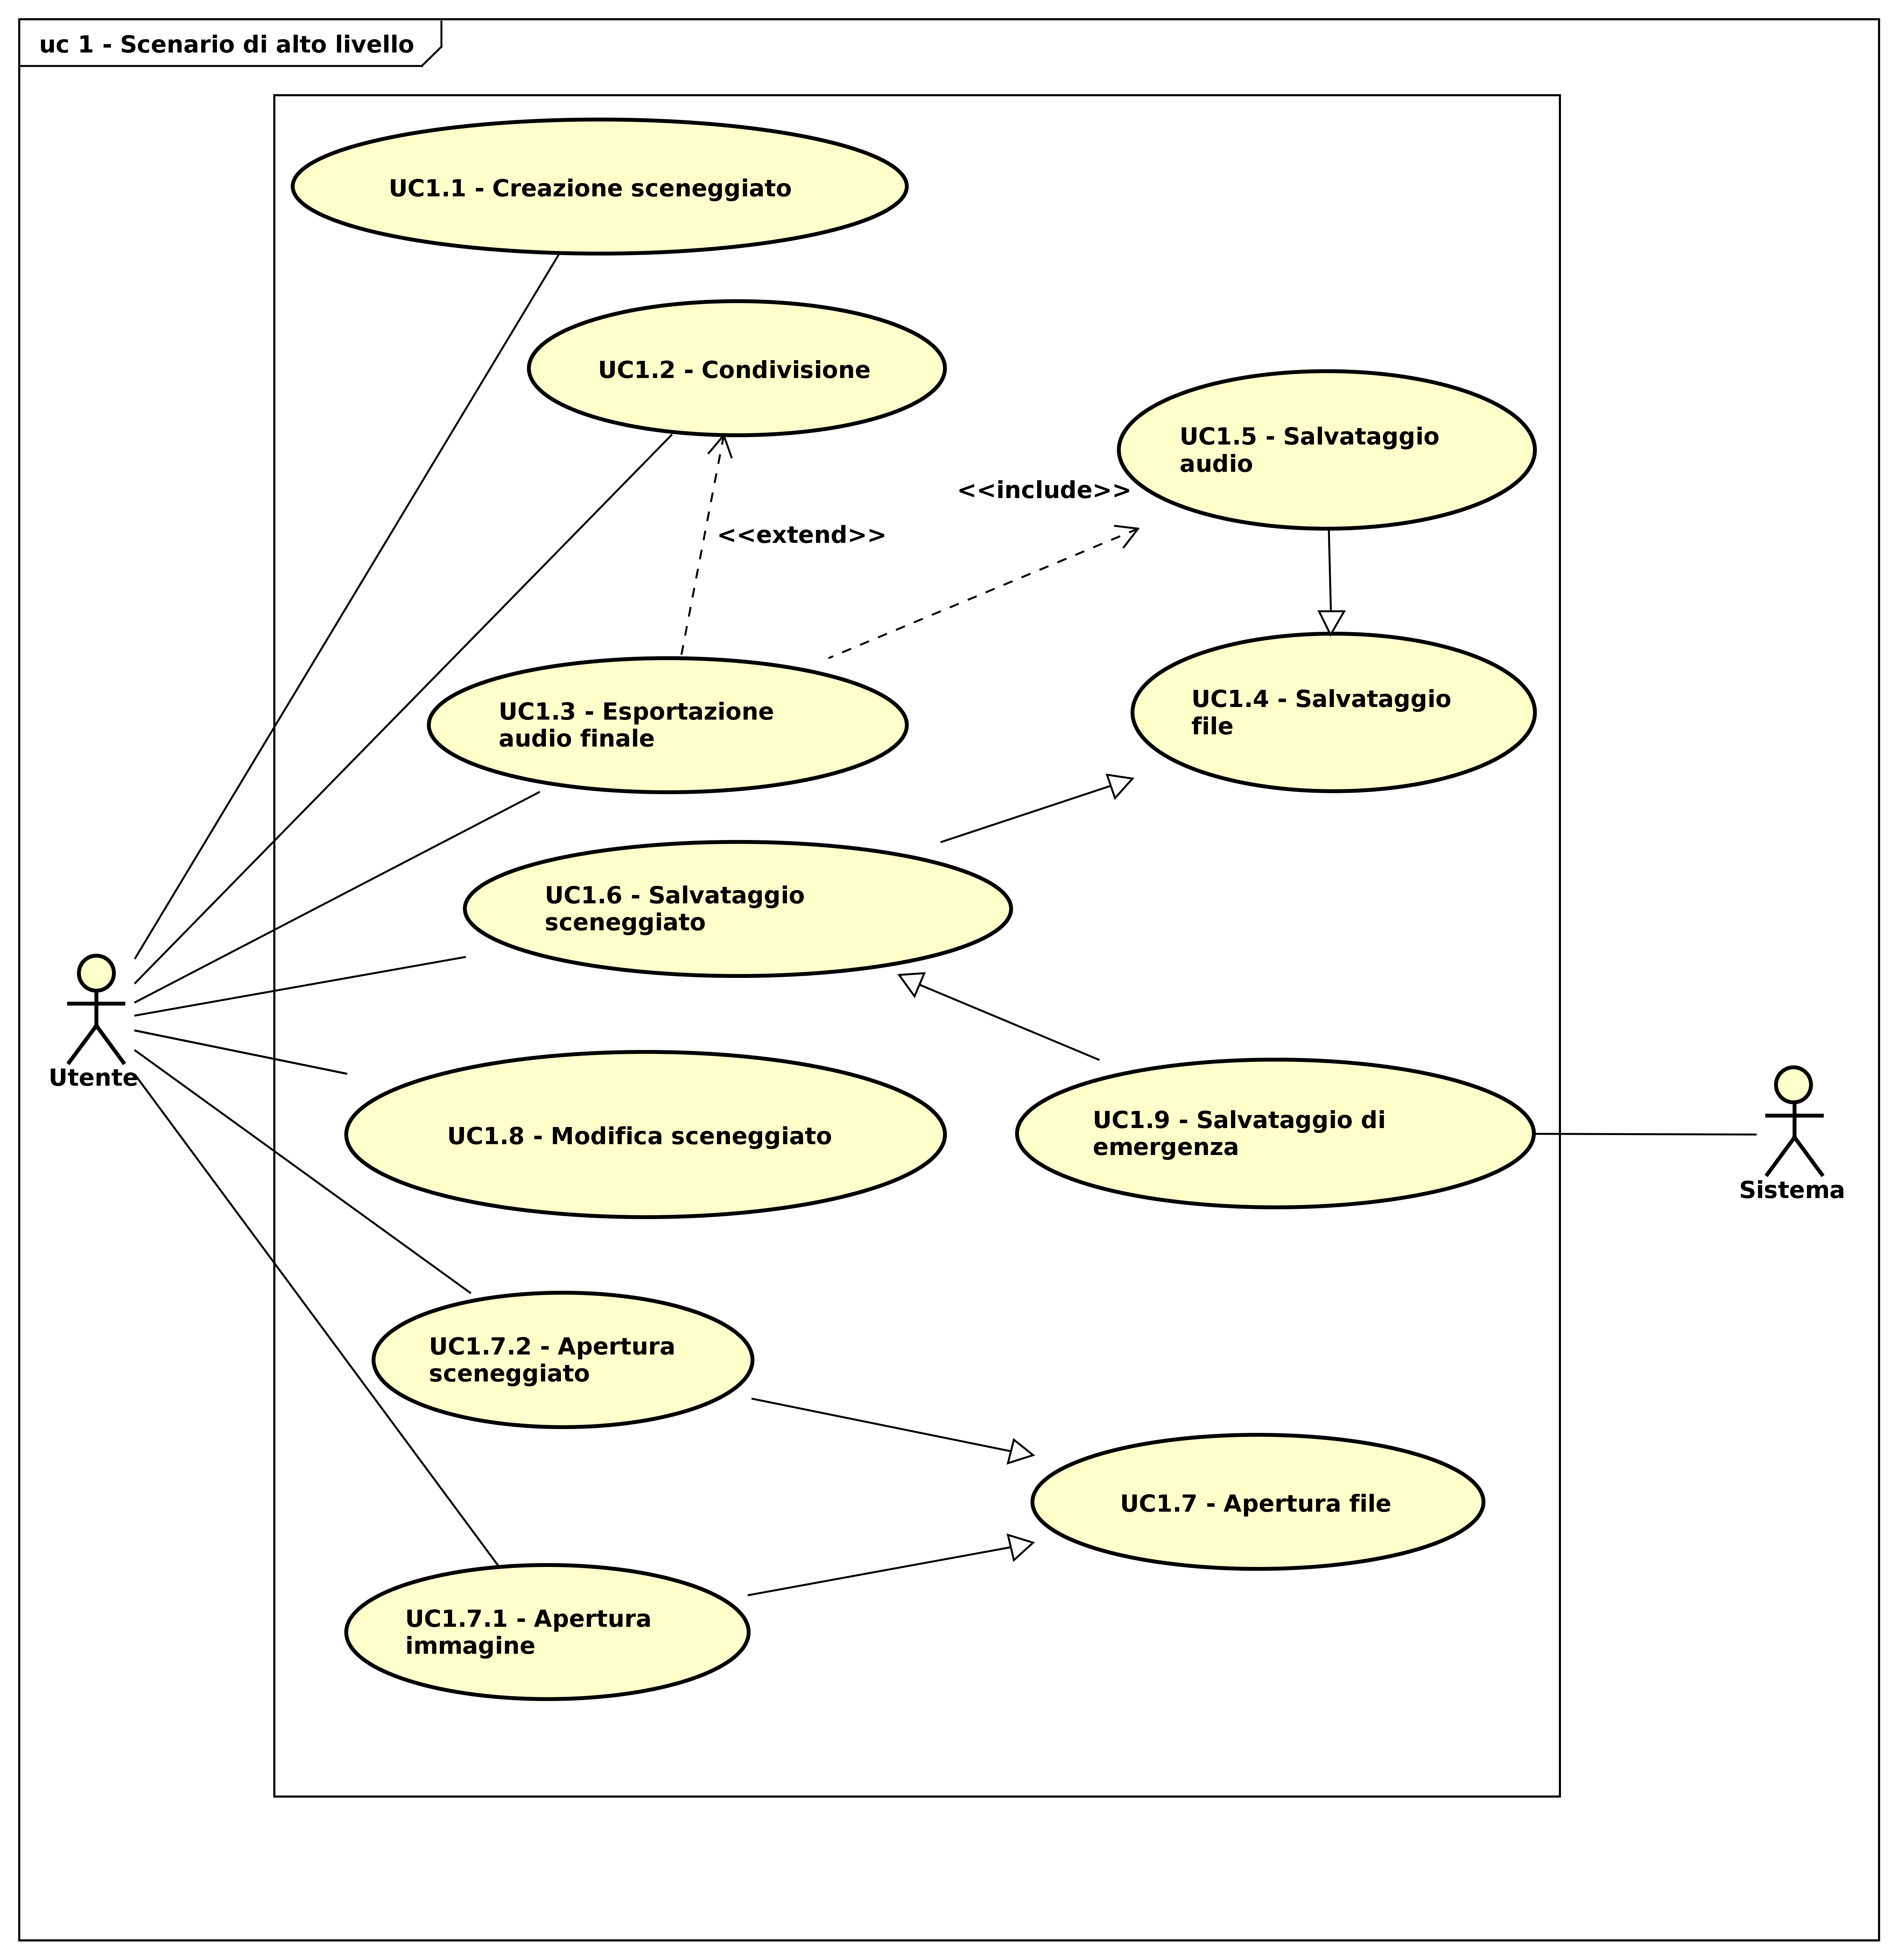
\includegraphics[scale=0.5]{UseCase_17_03_2016/immagini/uc_1_scenario_alto_livello.png}
\captionsetup{labelfont=bf}
\caption{Caso d'uso UC1}
\end{figure}

\begin{itemize}
\item \textbf{Attore}: Utente;
\item \textbf{Scopo e descrizione}: l'utente ha avviato correttamente l'applicazione per creare sceneggiati e questa è pronta all'uso. Possono essere effettuate diverse operazioni: l'utente può creare un nuovo sceneggiato oppure modificarne uno già iniziato; può salvare il suo lavoro, esportarlo in formato audio e condividerlo.
\item \textbf{Precondizione}: il programma è stato avviato ed è pronto all'uso;
\item \textbf{Flusso principale degli eventi}:
\begin{enumerate}
\item L'utente può creare un nuovo sceneggiato o lavorare su uno già iniziato (UC1.1 - UC1.8);
\item L'utente può esportare lo sceneggiato creato (UC1.3);
\item L'utente può salvare lo sceneggiato creato (UC1.6);
\item L'utente può condividere il file audio dello sceneggiato creato (UC1.2).
\end{enumerate}
\item \textbf{Estensioni}: la condivisione sarà disponibile solo dopo l'esportazione di un file in formato audio (UC1.2).
\item \textbf{Postcondizione}: il sistema ha ottenuto le informazioni sulle operazioni che
l'utente desidera eseguire.
\end{itemize}

\subsection{Caso d'uso UC1.1: Creazione sceneggiato}

\begin{figure}[htbp]
\centering
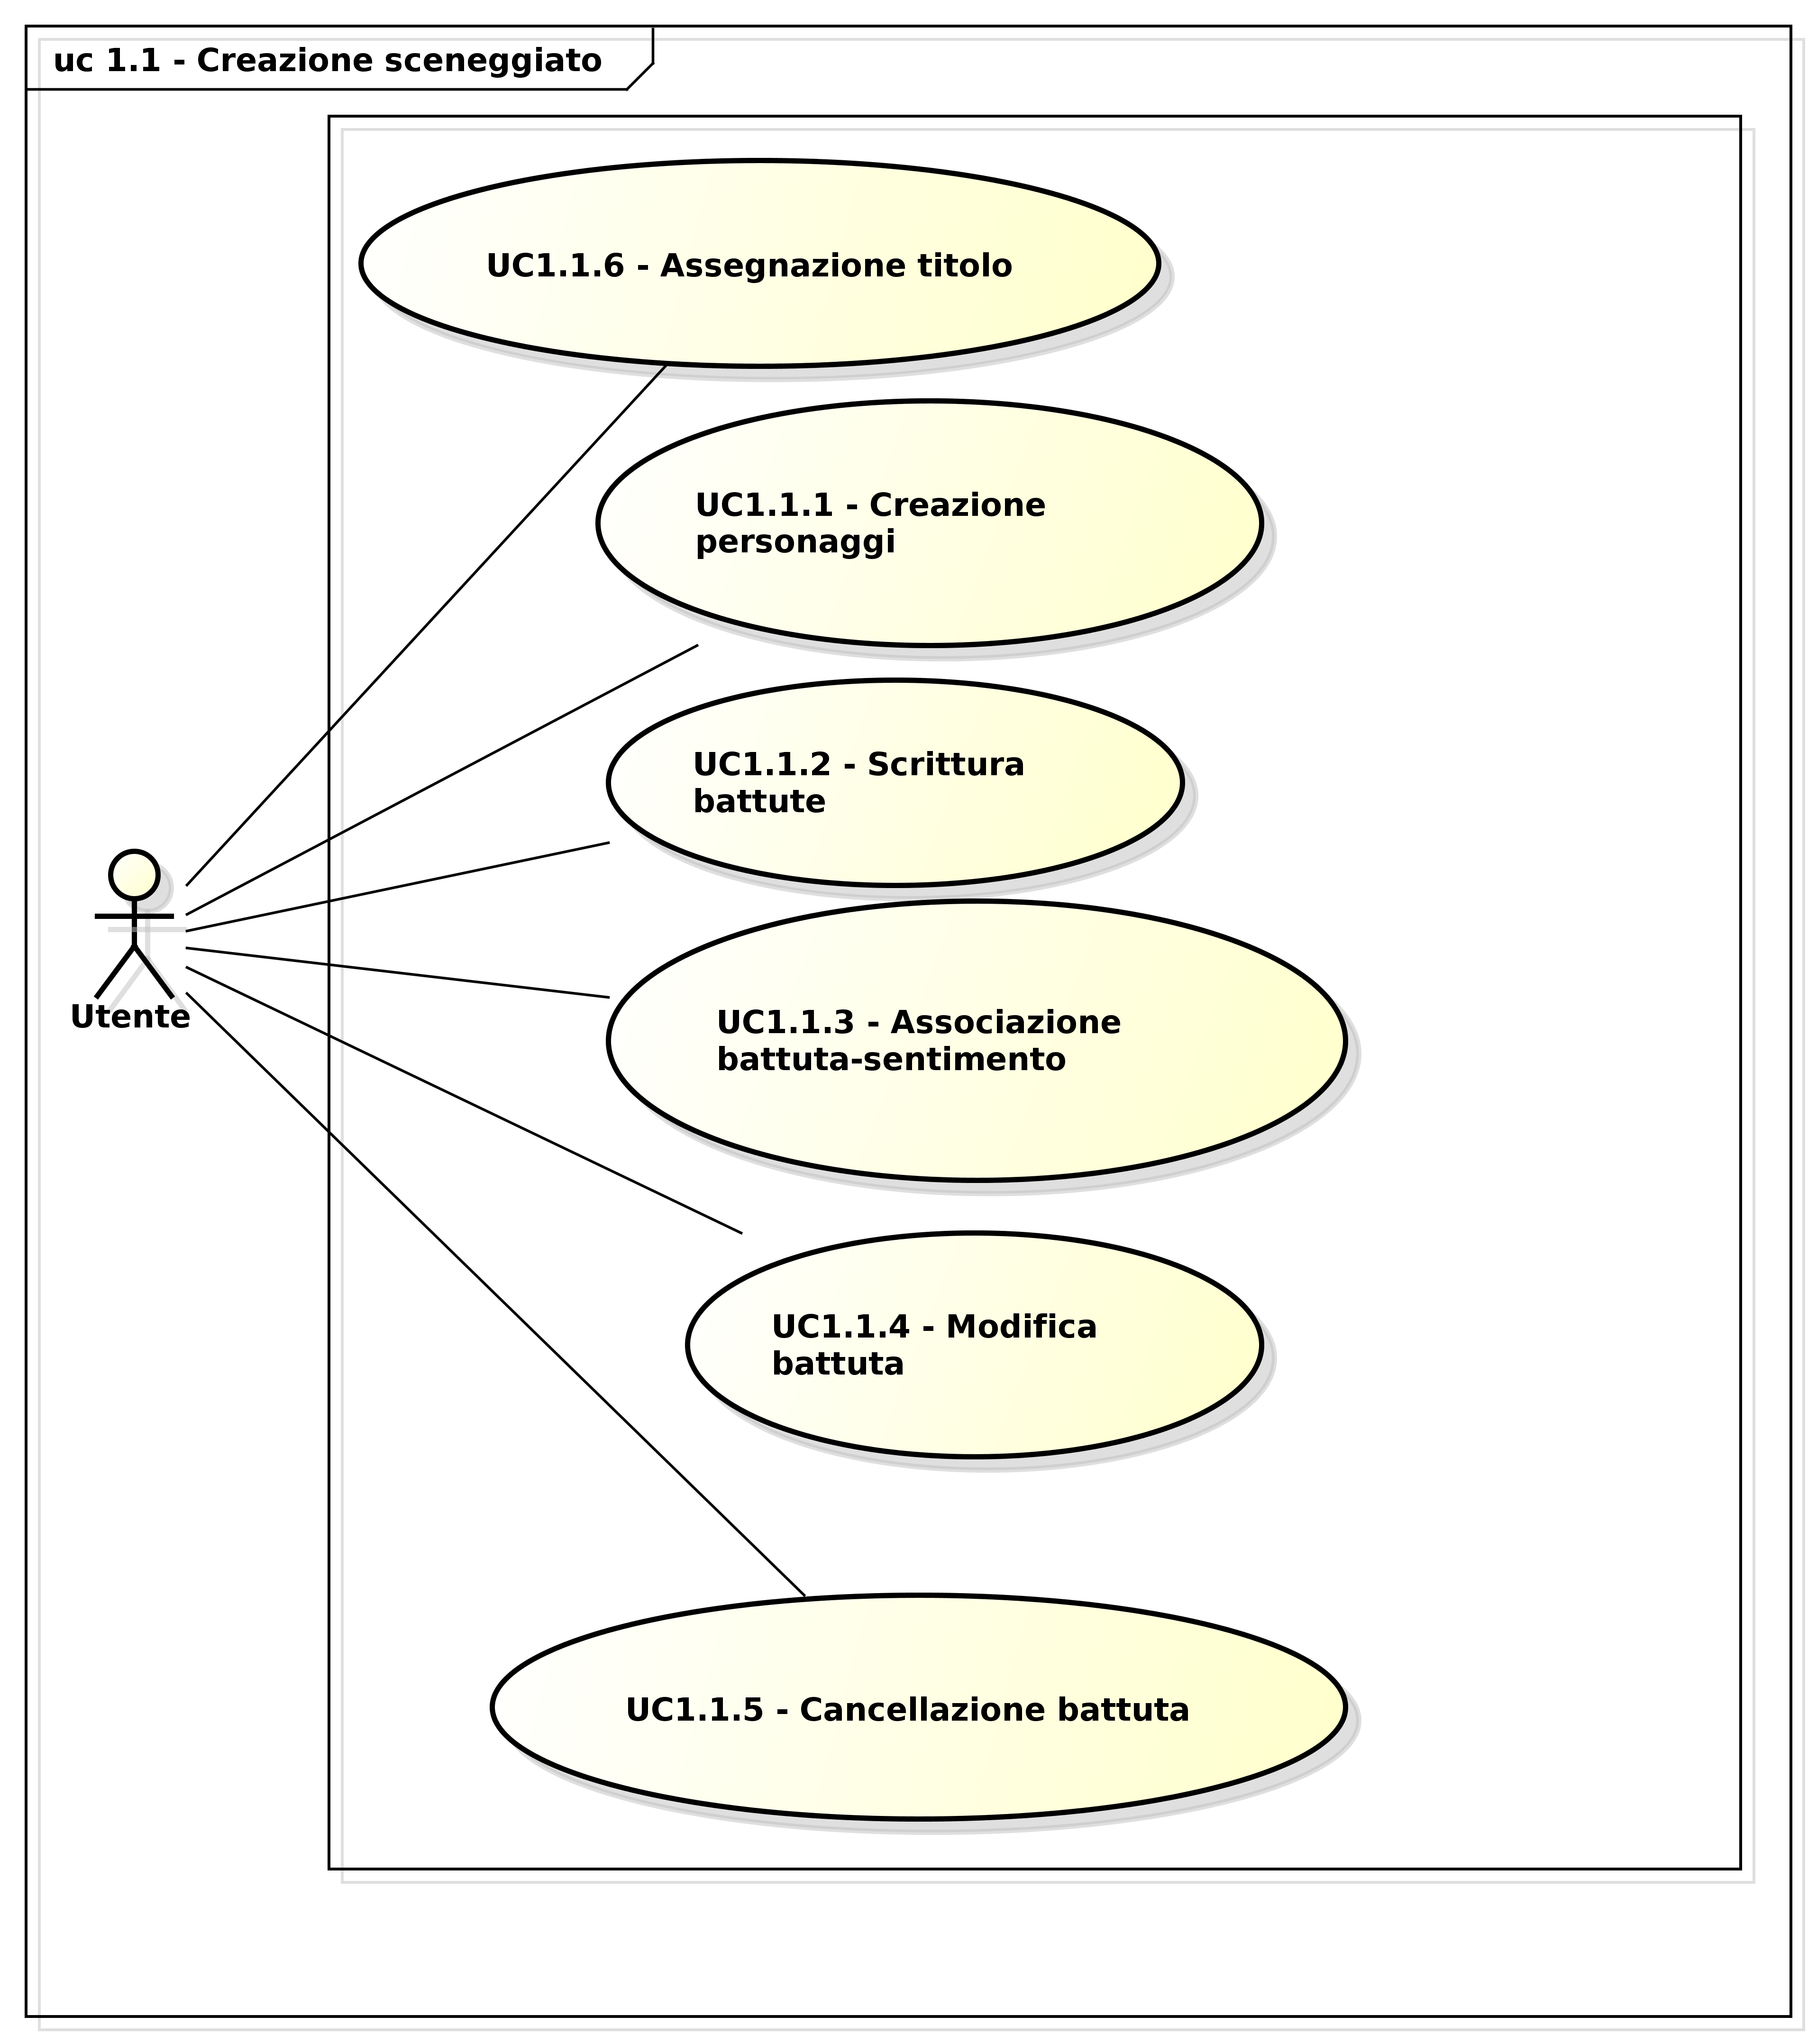
\includegraphics[scale=0.5]{UseCase_17_03_2016/immagini/uc_1_1_creazione_sceneggiato.png}
\captionsetup{labelfont=bf}
\caption{Caso d'uso UC1.1}
\end{figure}

\begin{itemize}
\item \textbf{Attore}: Utente;
\item \textbf{Scopo e descrizione}: l'utente ha scelto di creare un nuovo sceneggiato;
\item \textbf{Precondizione}: il sistema è pronto a creare un nuovo file;
\item \textbf{Flusso principale degli eventi}:
\begin{enumerate}
\item L'utente può assegnare un titolo al nuovo sceneggiato (UC1.1.6);
\item L'utente può creare i personaggi dello sceneggiato (UC1.1.1);
\item L'utente può scrivere le battute dello sceneggiato (UC1.1.2);
\item L'utente può associare un sentimento ad una battuta (UC1.1.3);
\end{enumerate}
\item \textbf{Scenari alternativi}: viene annullata la creazione del nuovo file se esiste già un altro sceneggiato salvato con lo stesso nome di quello appena creato; 
\item \textbf{Postcondizione}: Il sistema ha creato il nuovo file.
\end{itemize}

\subsection{Caso d'uso UC1.1.1: Creazione personaggi}

\begin{figure}[htbp]
\centering
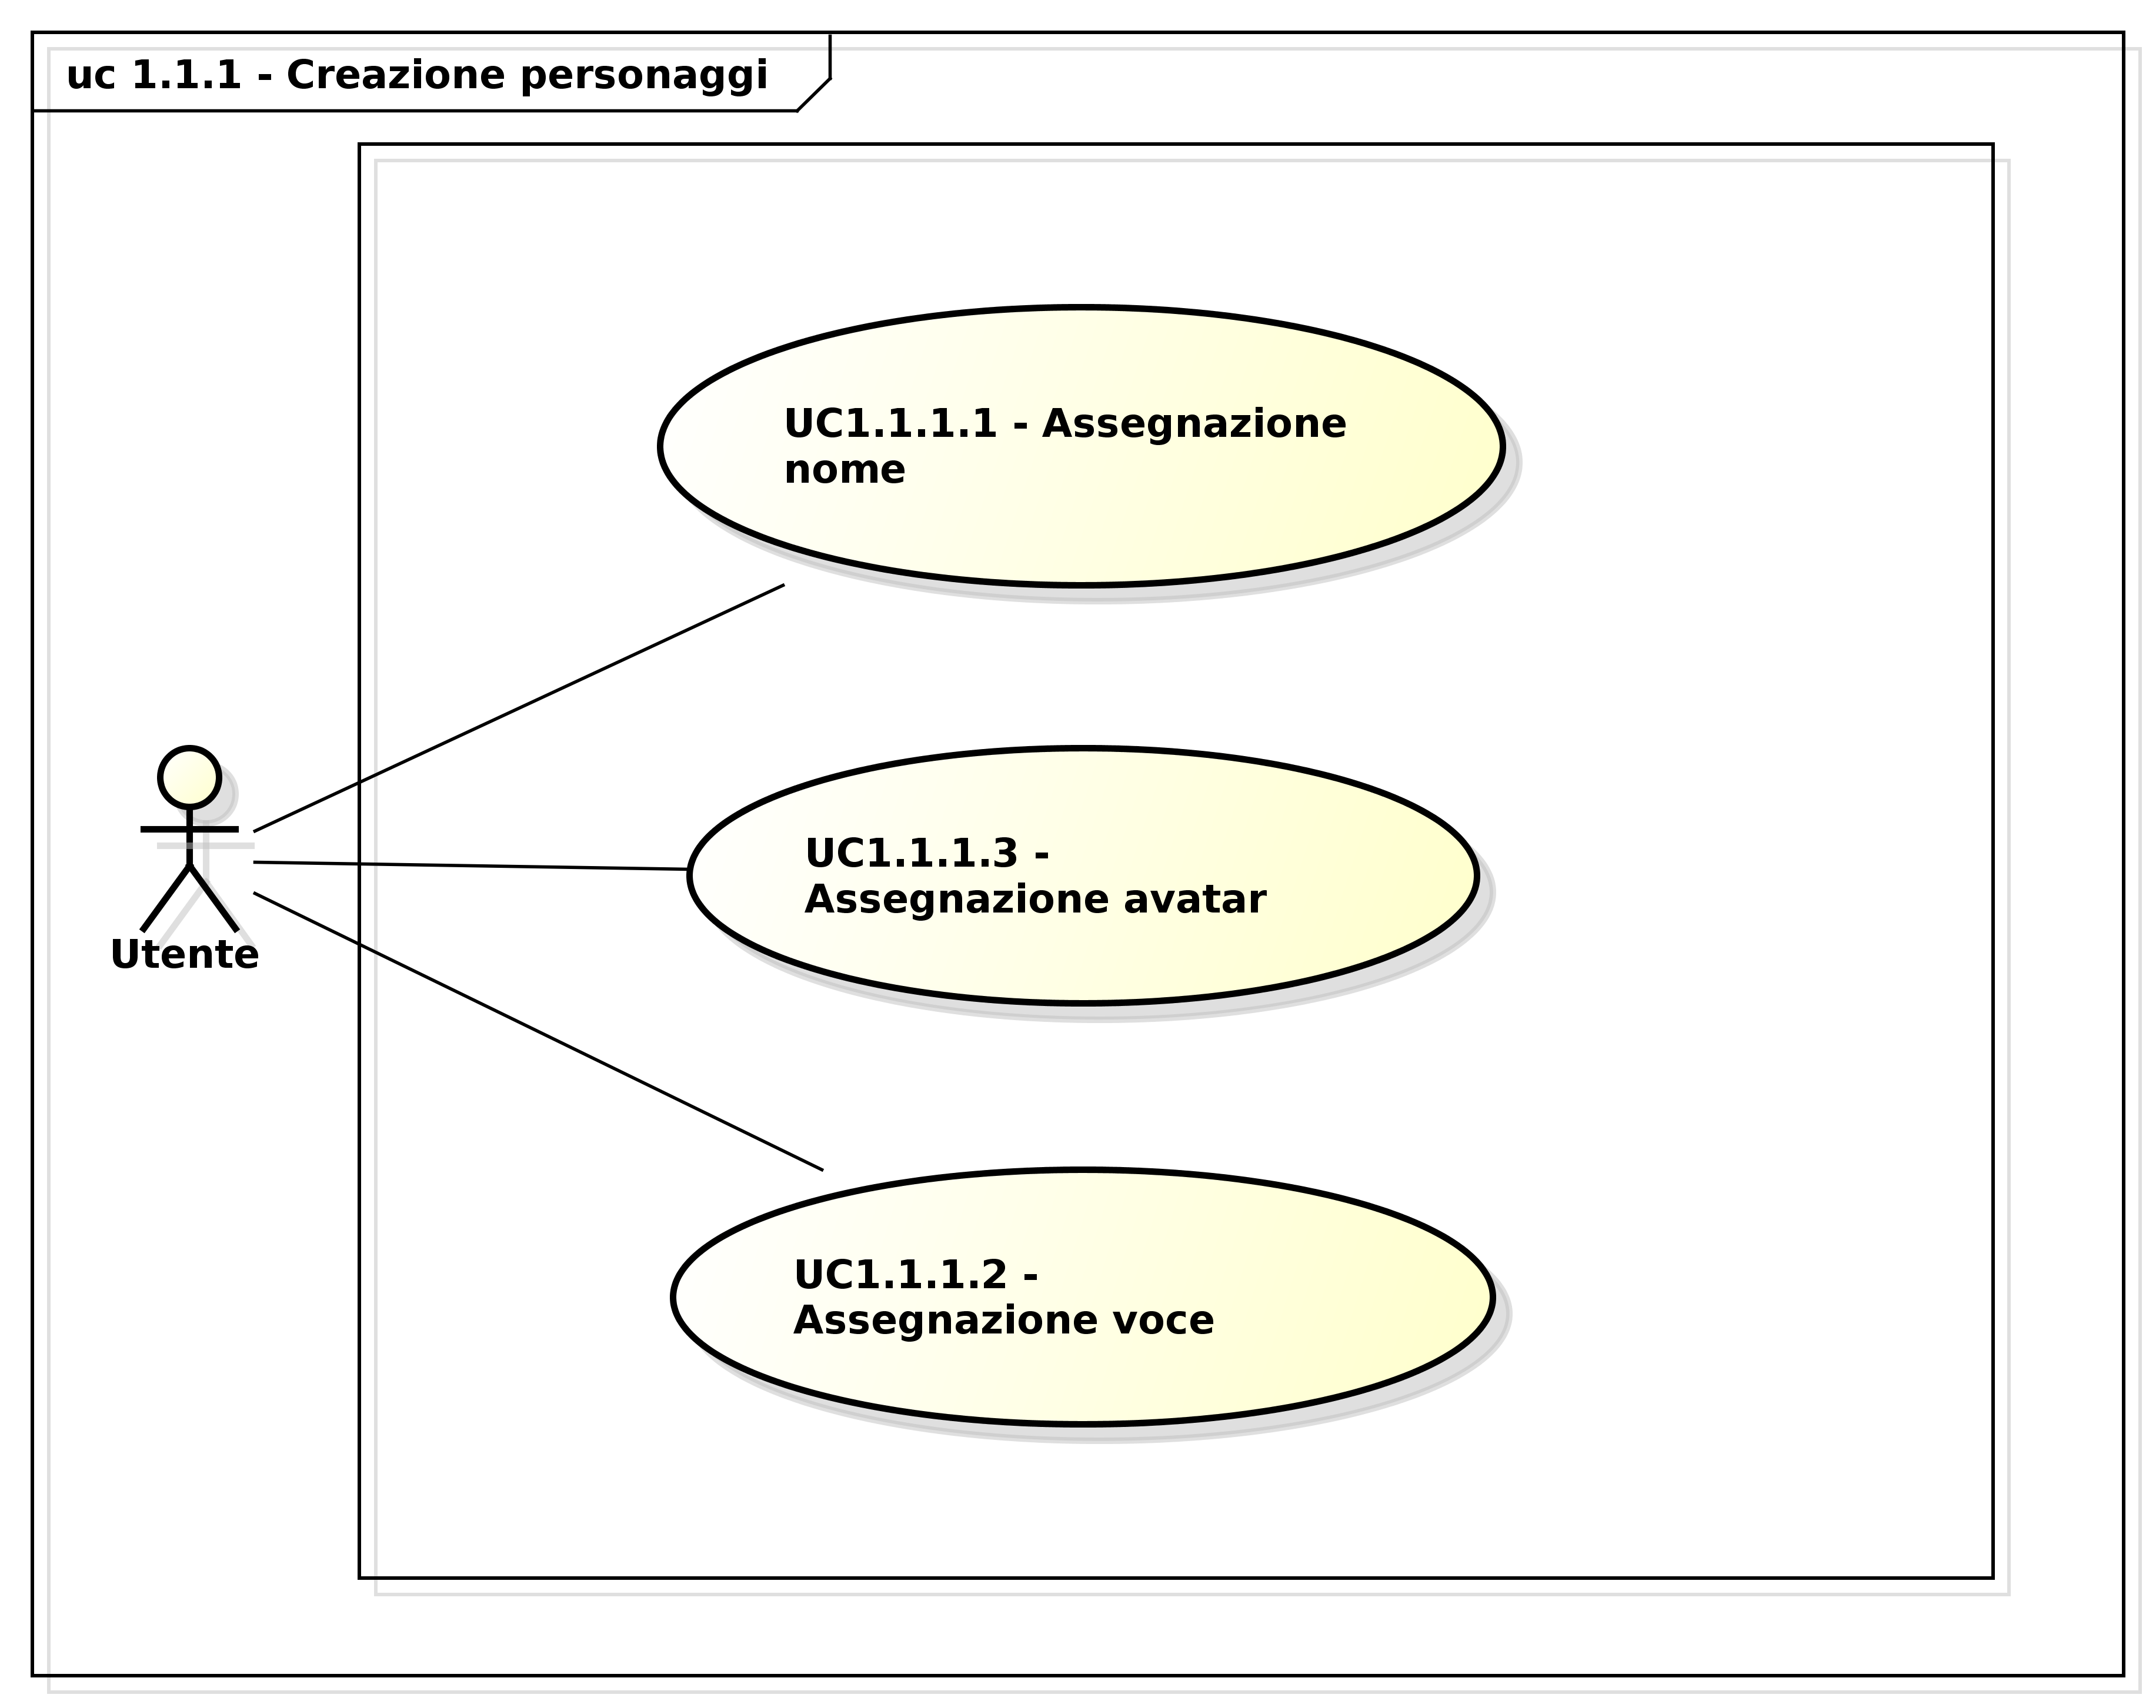
\includegraphics[scale=0.5]{UseCase_17_03_2016/immagini/uc_1_1_1_creazione_personaggi.png}
\captionsetup{labelfont=bf}
\caption{Caso d'uso UC1.1.1}
\end{figure}

\begin{itemize}
\item \textbf{Attore}: Utente;
\item \textbf{Scopo e descrizione}: l'utente può creare un nuovo personaggio per il suo sceneggiato associandoci un nome, un avatar e una voce;
\item \textbf{Precondizione}: il sistema è pronto a creare un nuovo personaggio;
\item \textbf{Flusso principale degli eventi}:
\begin{enumerate}
\item L'utente assegna un nome al nuovo personaggio (UC1.1.1.1);
\item L'utente assegna un avatar al nuovo personaggio (UC1.1.1.3);
\item L'utente assegna una voce al nuovo personaggio (UC1.1.1.2);
\end{enumerate} 
\item \textbf{Scenari alternativi}: la creazione può fallire nel caso in cui esista già un personaggio nel corrente sceneggiato con lo stesso nome di quello dato a quello nuovo;
\item \textbf{Postcondizione}: il sistema crea un nuovo personaggio.
\end{itemize}

\subsection{Caso d'uso UC1.1.2: Assegnazione voce}

\begin{figure}[htbp]
\centering
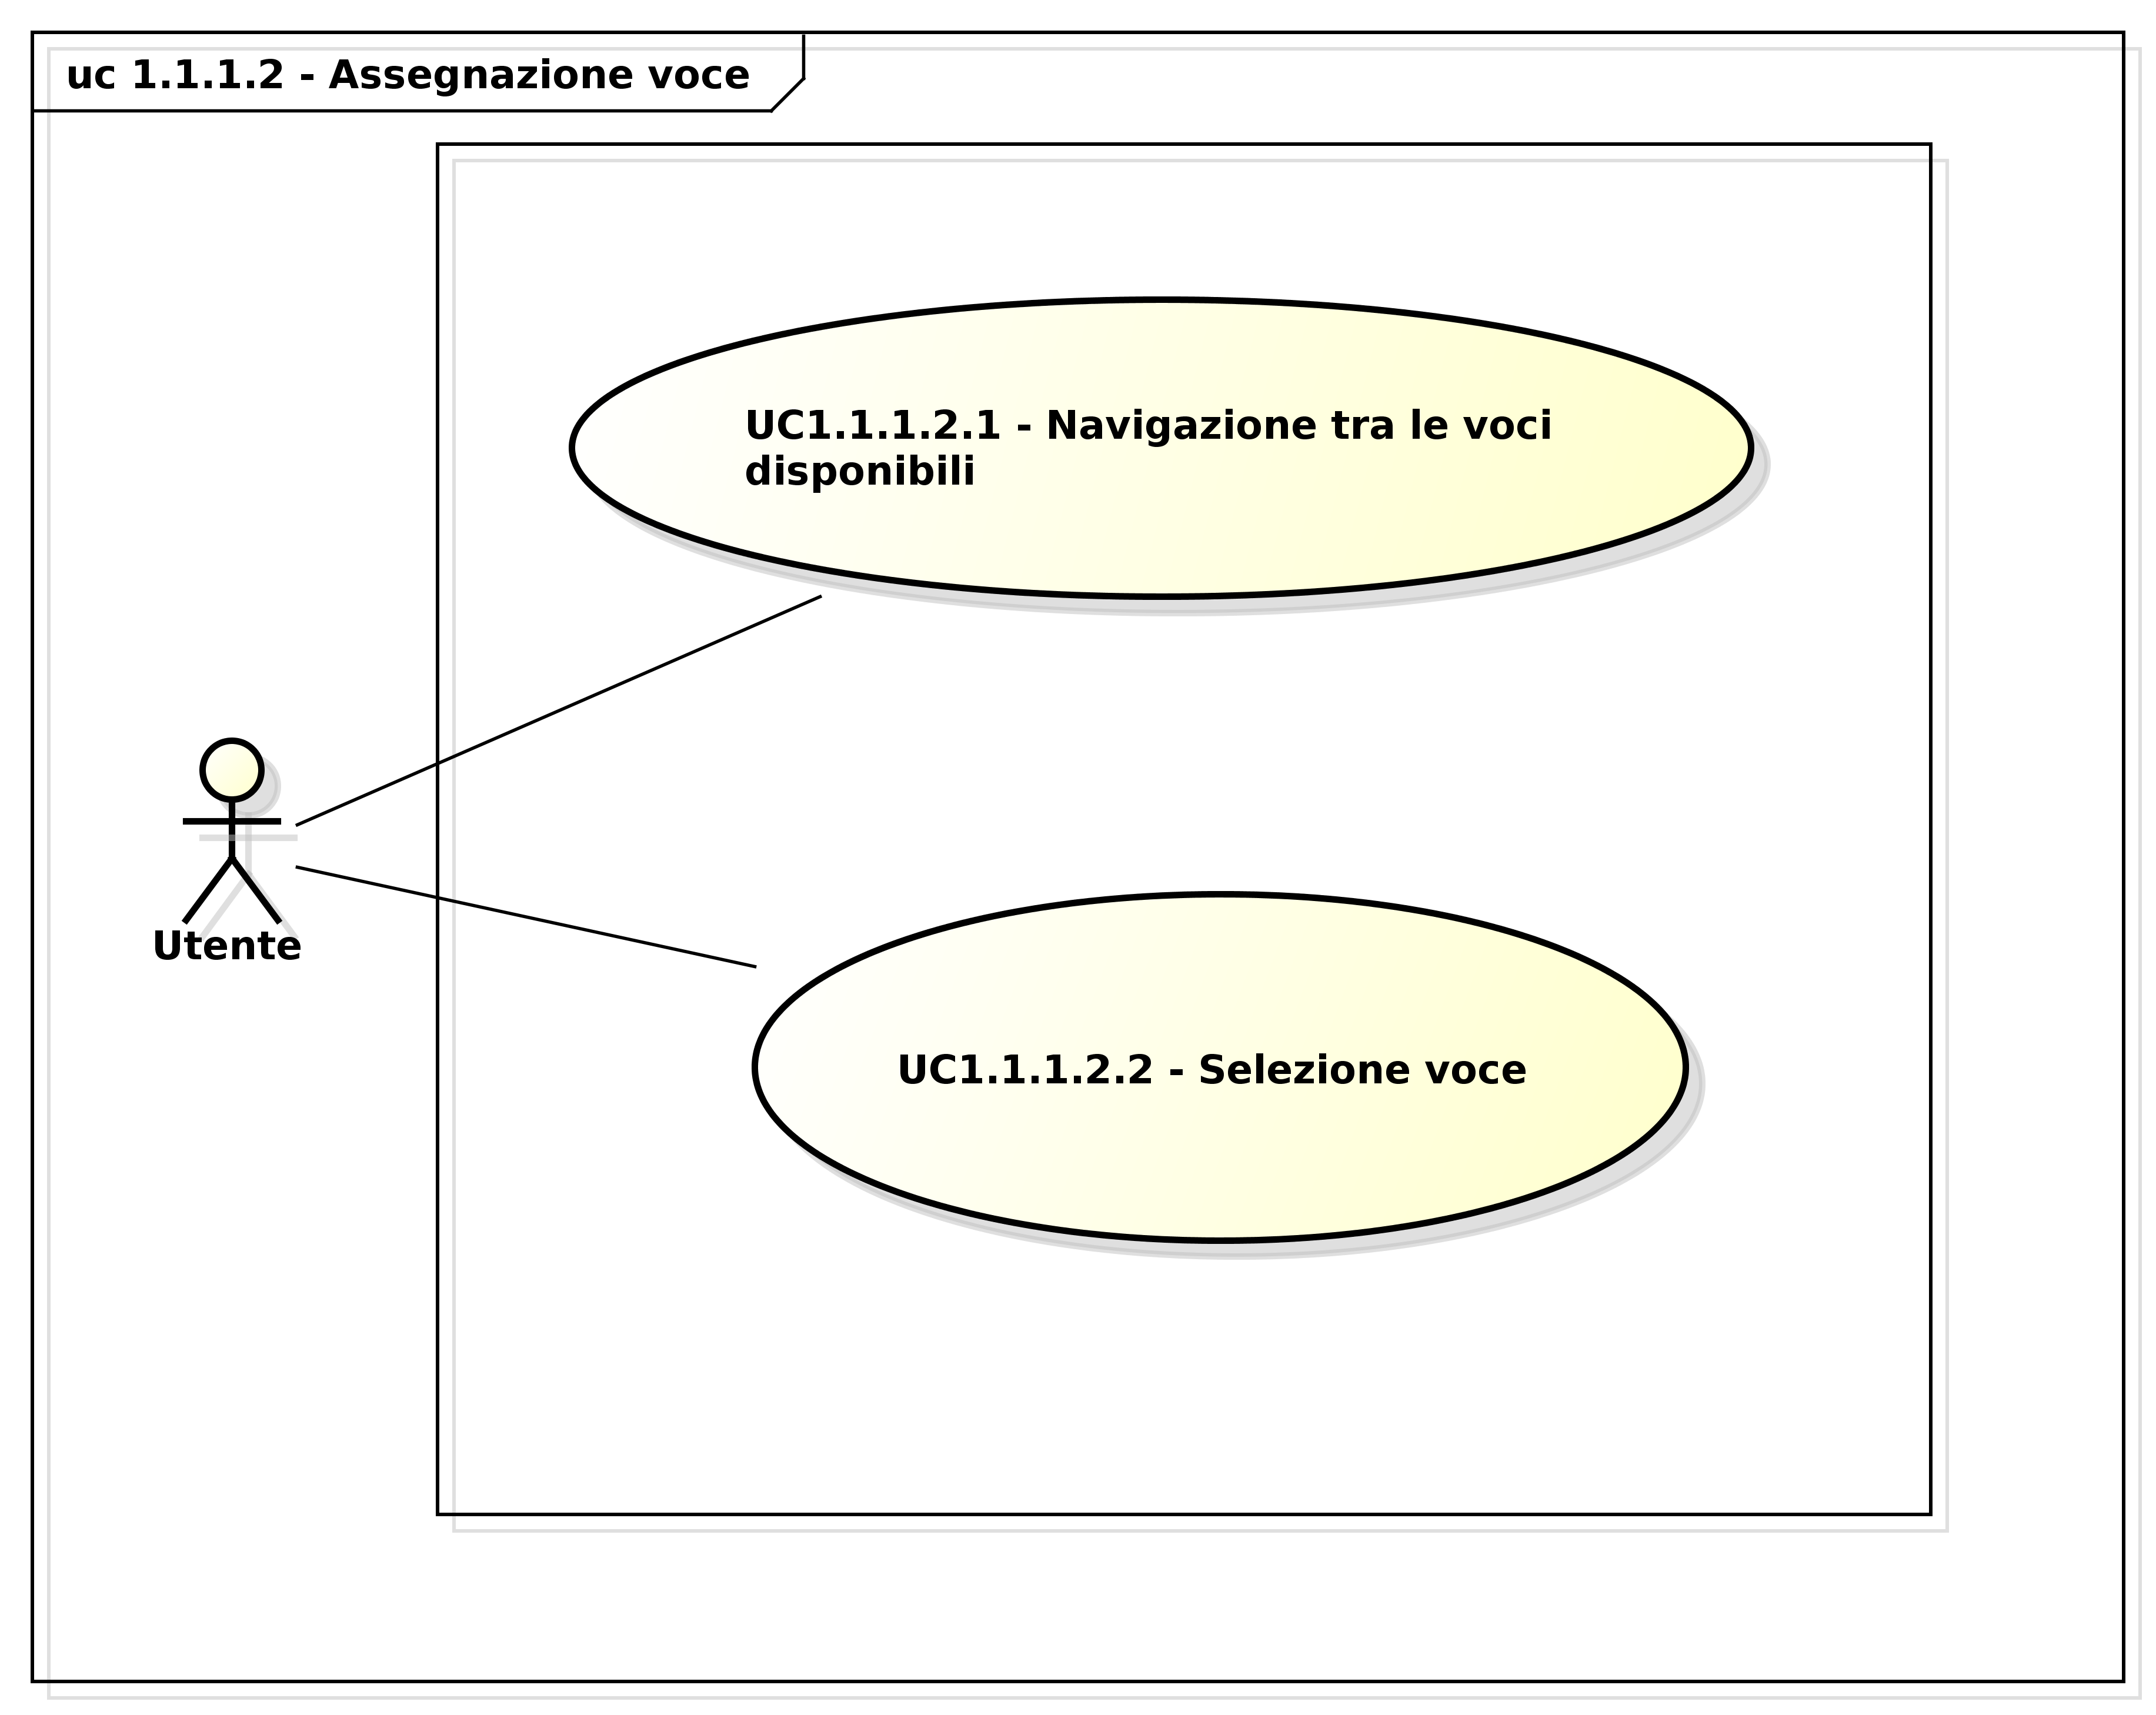
\includegraphics[scale=0.5]{UseCase_17_03_2016/immagini/uc_1_1_1_2_assegnazione_voce.png}
\captionsetup{labelfont=bf}
\caption{Caso d'uso UC1.1.2}
\end{figure}

\begin{itemize}
\item \textbf{Attore}: Utente;
\item \textbf{Scopo e descrizione}: l'utente assegna al personaggio creato una voce tra quelle disponibili; 
\item \textbf{Precondizione}: il sistema è pronto a ricevere la selezione di una voce;
\item \textbf{Flusso principale degli eventi}:
\begin{enumerate}
\item L'utente può navigare tra le voci disponibili (UC1.1.1.2.1);
\item L'utente seleziona una voce (UC1.1.1.2.1).
\end{enumerate}
\item \textbf{Postcondizione}: il sistema associa la voce selezionata al personaggio.
\end{itemize}

\subsection{Caso d'uso UC1.1.2: Scrittura battute}

\begin{figure}[htbp]
\centering
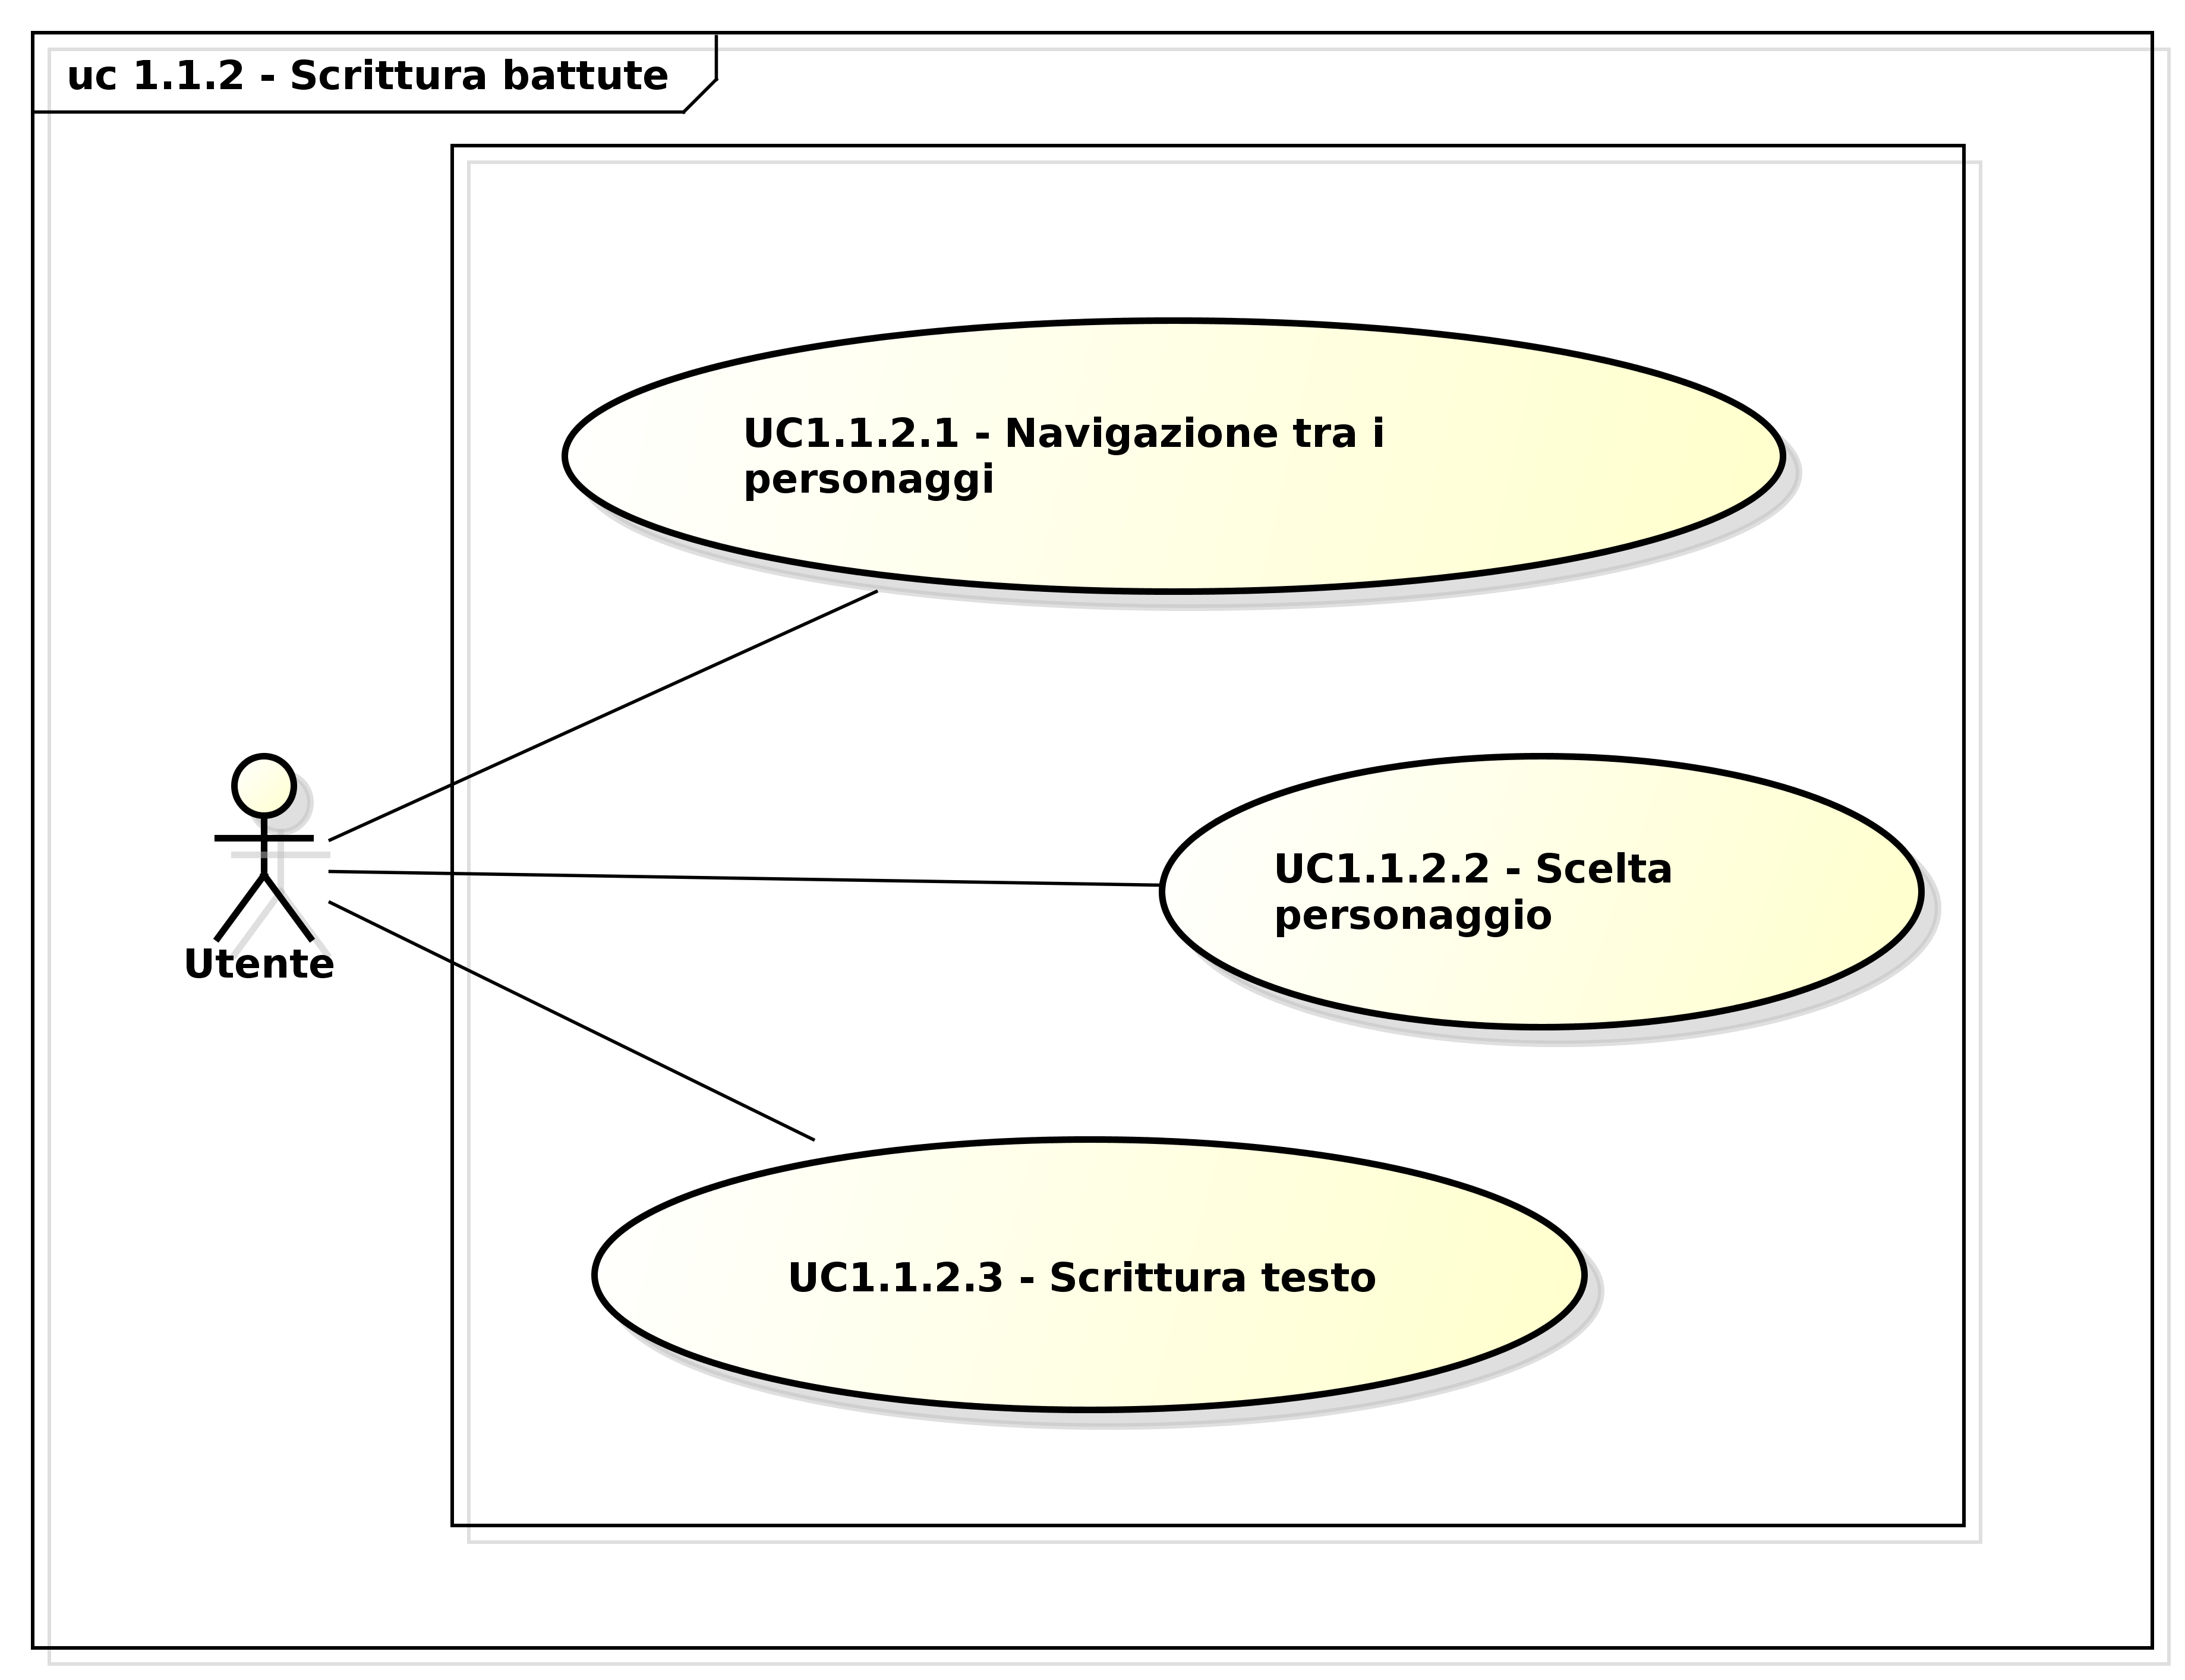
\includegraphics[scale=0.5]{UseCase_17_03_2016/immagini/uc_1_1_2_scrittura_battute.png}
\captionsetup{labelfont=bf}
\caption{Caso d'uso UC1.1.2}
\end{figure}

\begin{itemize}
\item \textbf{Attore}: Utente;
\item \textbf{Scopo e descrizione}: l'utente può digitare il testo di una nuova battuta e assegnarla ad un personaggio;
\item \textbf{Precondizione}: il sistema è pronto a ricevere il testo per la creazione di una nuova battuta;
\item \textbf{Flusso principale degli eventi}:
\begin{enumerate}
\item L'utente scrive il testo della nuova battuta (UC1.1.2.3);
\item L'utente naviga tra i personaggi disponibili (UC1.1.2.1);
\item L'utente seleziona il personaggio a cui associare la battuta (UC1.1.2.2).
\end{enumerate} 
\item \textbf{Postcondizione}: \'E stata creata una nuova battuta;
\end{itemize}

\subsection{Caso d'uso UC1.1.3: Associazione battuta-sentimento}

\begin{figure}[htbp]
\centering
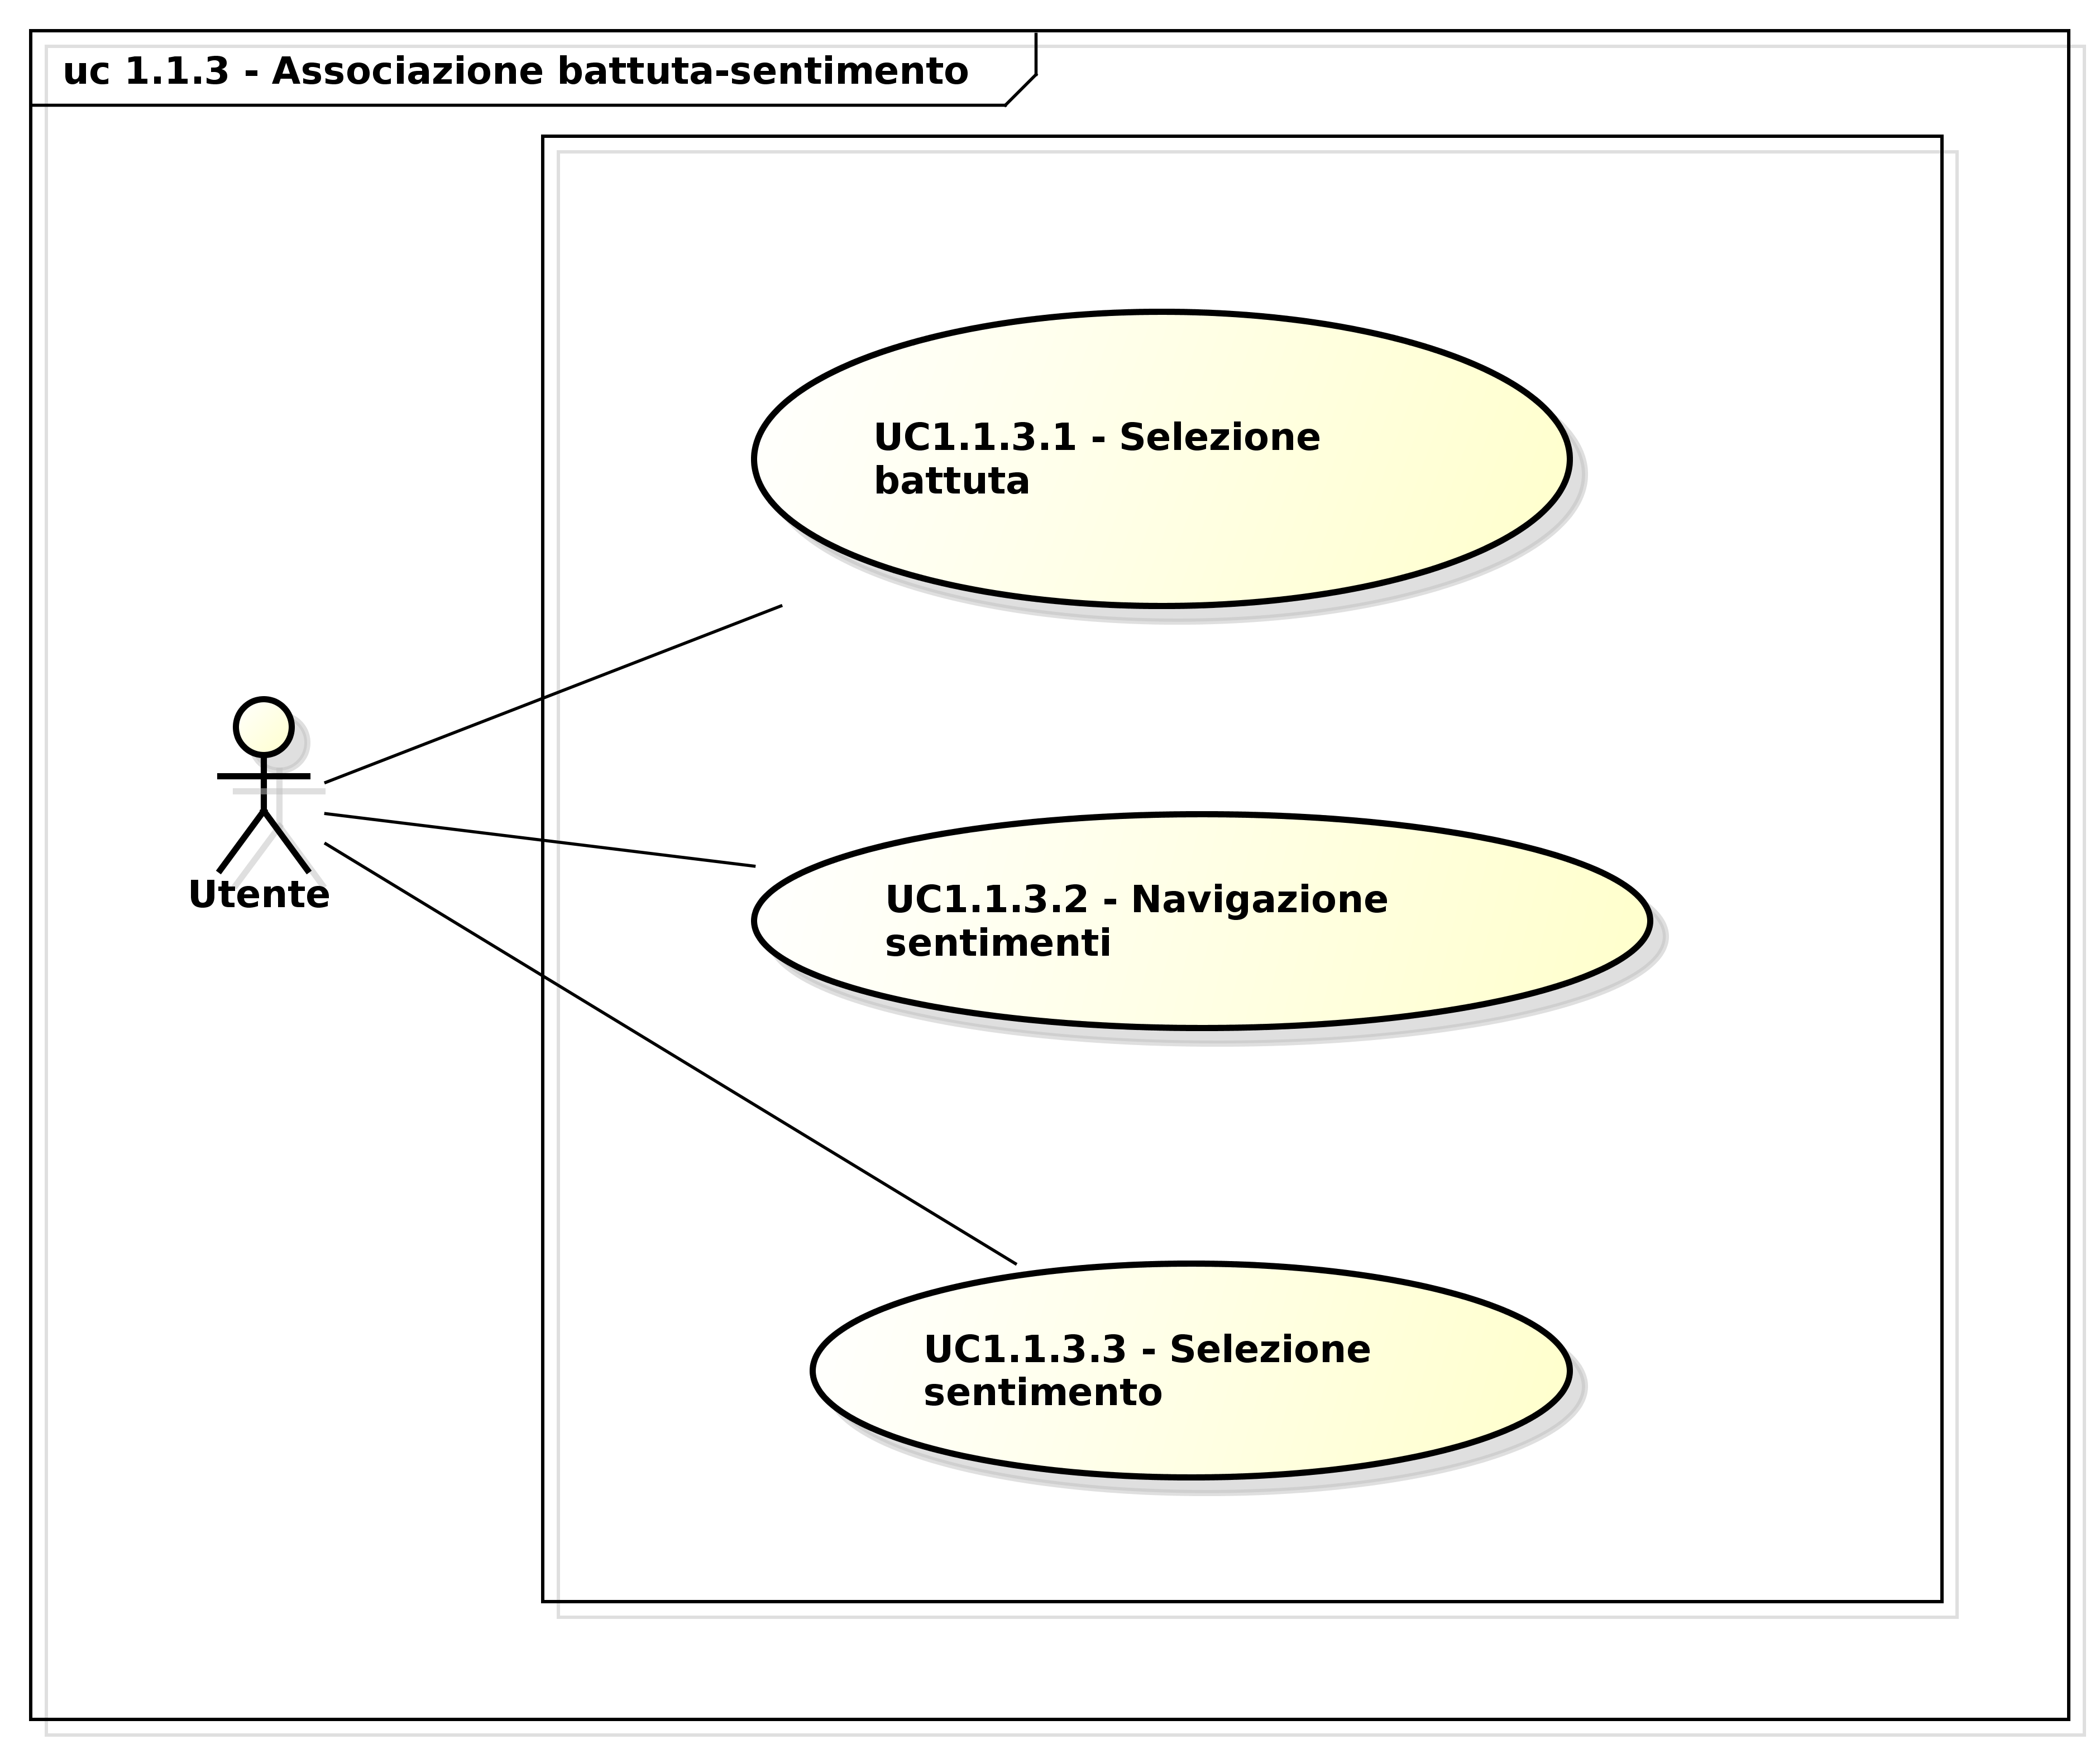
\includegraphics[scale=0.5]{UseCase_17_03_2016/immagini/uc_1_1_3_associazione_battuta_sentimento.png}
\captionsetup{labelfont=bf}
\caption{Caso d'uso UC1.1.3}
\end{figure}

\begin{itemize}
\item \textbf{Attore}: Utente;
\item \textbf{Scopo e descrizione}: l'utente, dopo aver creato una battuta, può decidere di associarle una sentimento navigando tra quelli disponibili;
\item \textbf{Precondizione}: una battuta è stata creata;
\item \textbf{Flusso principale degli eventi}:
\begin{enumerate}
\item L'utente seleziona la battuta (UC1.1.3.1);
\item L'utente naviga tra i sentimenti disponibili (UC1.1.3.2);
\item L'utente seleziona il sentimento (UC1.1.3.3).
\end{enumerate}
\item \textbf{Postcondizione}: è stato assegnato un sentimento alla battuta selezionata.
\end{itemize}

\subsection{Caso d'uso UC1.1.4: Modifica battuta}

\begin{figure}[htbp]
\centering
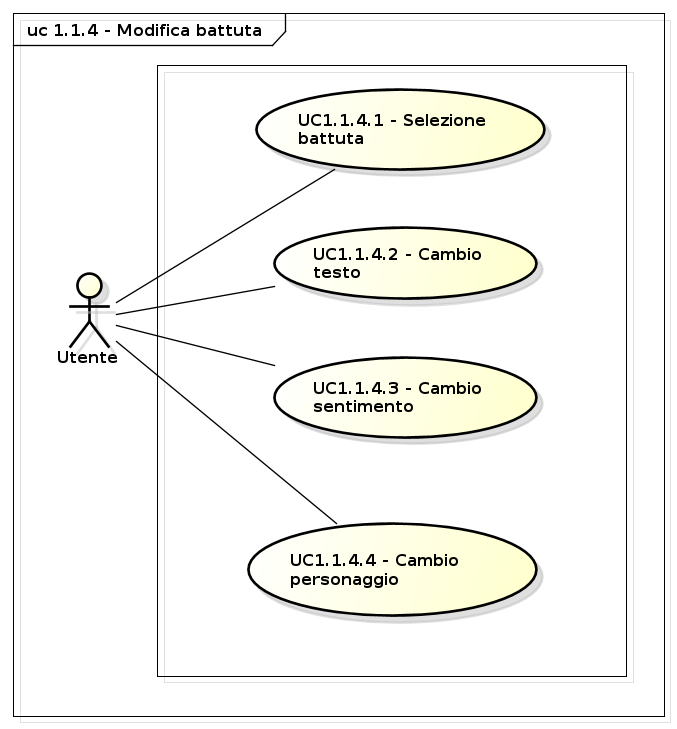
\includegraphics[scale=0.5]{UseCase_17_03_2016/immagini/uc_1_1_4_modifica_battuta.png}
\captionsetup{labelfont=bf}
\caption{Caso d'uso UC1.1.4}
\end{figure}

\begin{itemize}
\item \textbf{Attore}: Utente;
\item \textbf{Scopo e descrizione}: l'utente può modificare una battuta già creata cambiandone il testo o il sentimento associato o il personaggio; 
\item \textbf{Precondizione}: la battuta è stata creata correttamente;
\item \textbf{Flusso principale degli eventi}:
\begin{enumerate}
\item L'utente seleziona la battuta da modificare (UC1.1.4.1);
\item L'utente può scegliere se cambiarne il testo, il sentimento associato o il relativo personaggio (UC1.1.4.2 - UC1.1.4.3 - UC1.1.4.4).
\end{enumerate}
\item \textbf{Postcondizione}: la modifica è avvenuta correttamente.
\end{itemize}

\subsection{Caso d'uso UC1.2: Condivisione}

\begin{figure}[htbp]
\centering
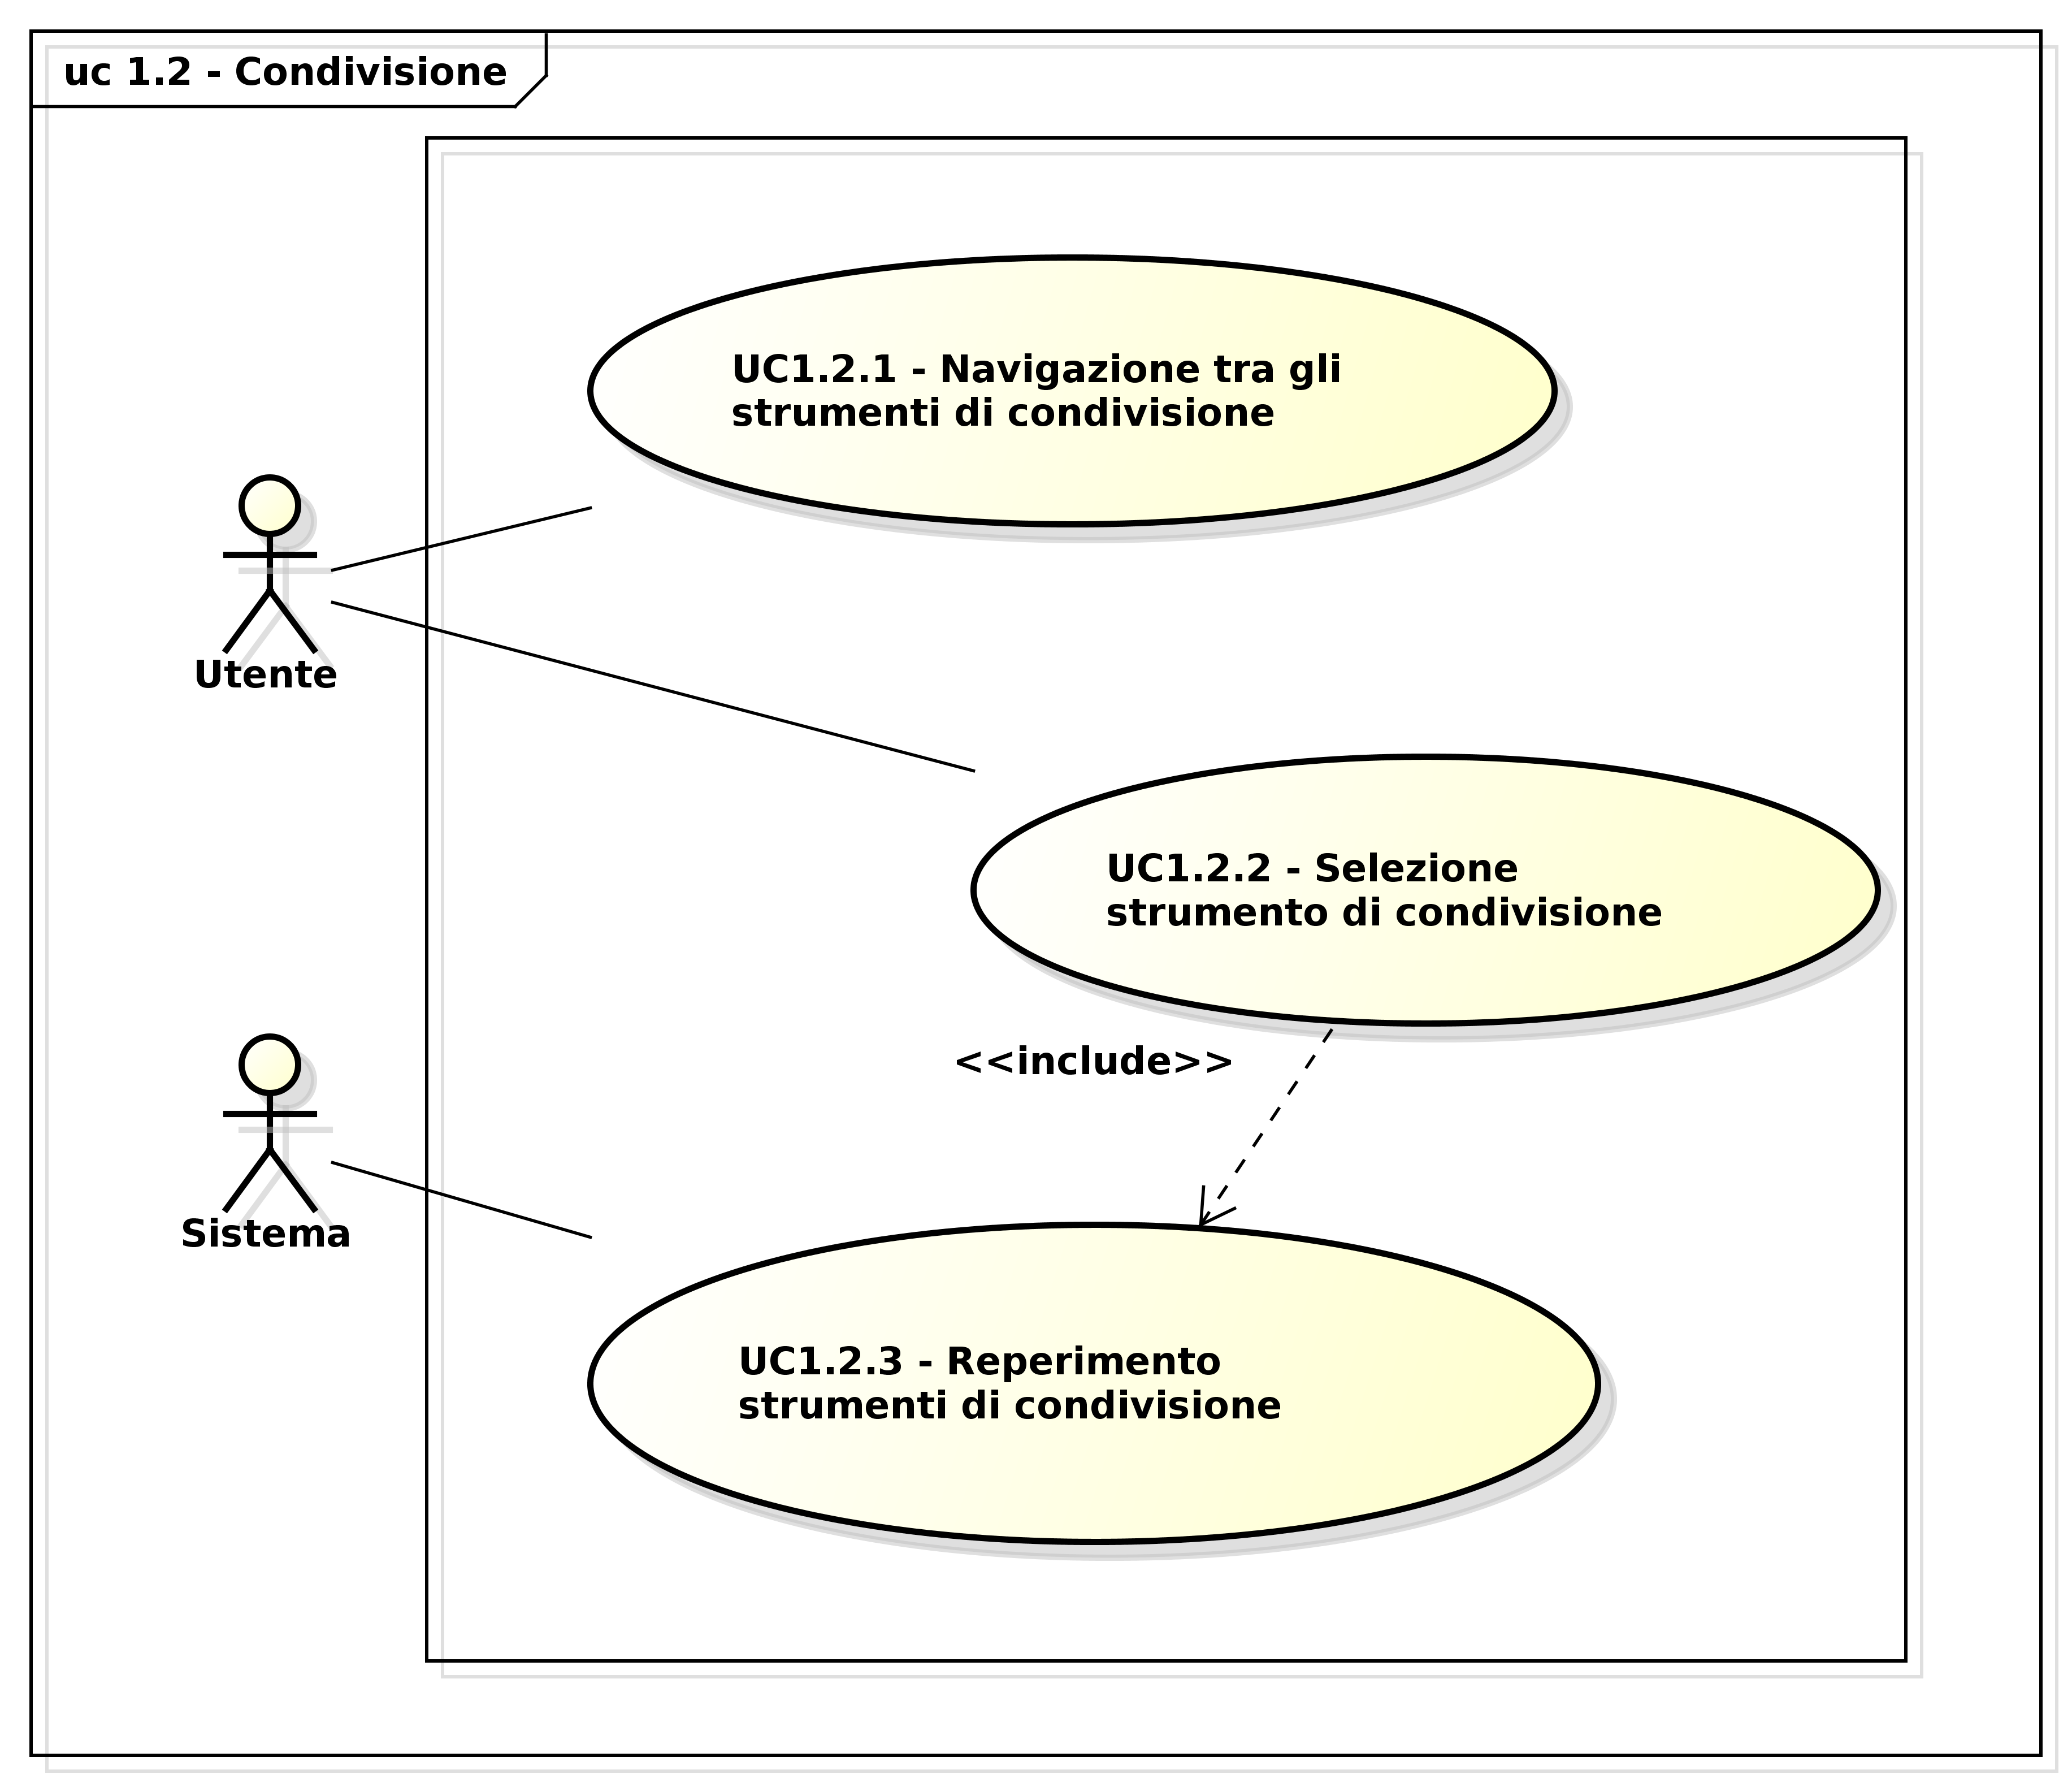
\includegraphics[scale=0.5]{UseCase_17_03_2016/immagini/uc_1_2_condivisione.png}
\captionsetup{labelfont=bf}
\caption{Caso d'uso UC1}
\end{figure}

\begin{itemize}
\item \textbf{Attori}: Utente, Sistema;
\item \textbf{Scopo e descrizione}: L'utente può condividere il file di esportazione relativo allo sceneggiato creato scegliendo uno tra gli strumenti di condivisione reperiti dal sistema;
\item \textbf{Precondizione}: l'esportazione dell'audio è andata a buon fine;
\item \textbf{Flusso principale degli eventi}:
\begin{enumerate}
\item Il sistema reperisce la lista degli strumenti di condivisione presenti nel dispositivo (UC1.2.3);
\item L'utente può navigare tra gli elementi della suddetta lista (UC1.2.1);
\item L'utente scegli uno tra gli elementi della lista (UC1.2.2).
\end{enumerate}
\item \textbf{Scenari alternativi}: il dispositivo non possiede alcuno strumento di condivisione;  
\item \textbf{Postcondizione}: l'audio verrà condiviso correttamente; 
\end{itemize}

\subsection{Caso d'uso UC1.3: Esportazione file audio}

\begin{figure}[htbp]
\centering
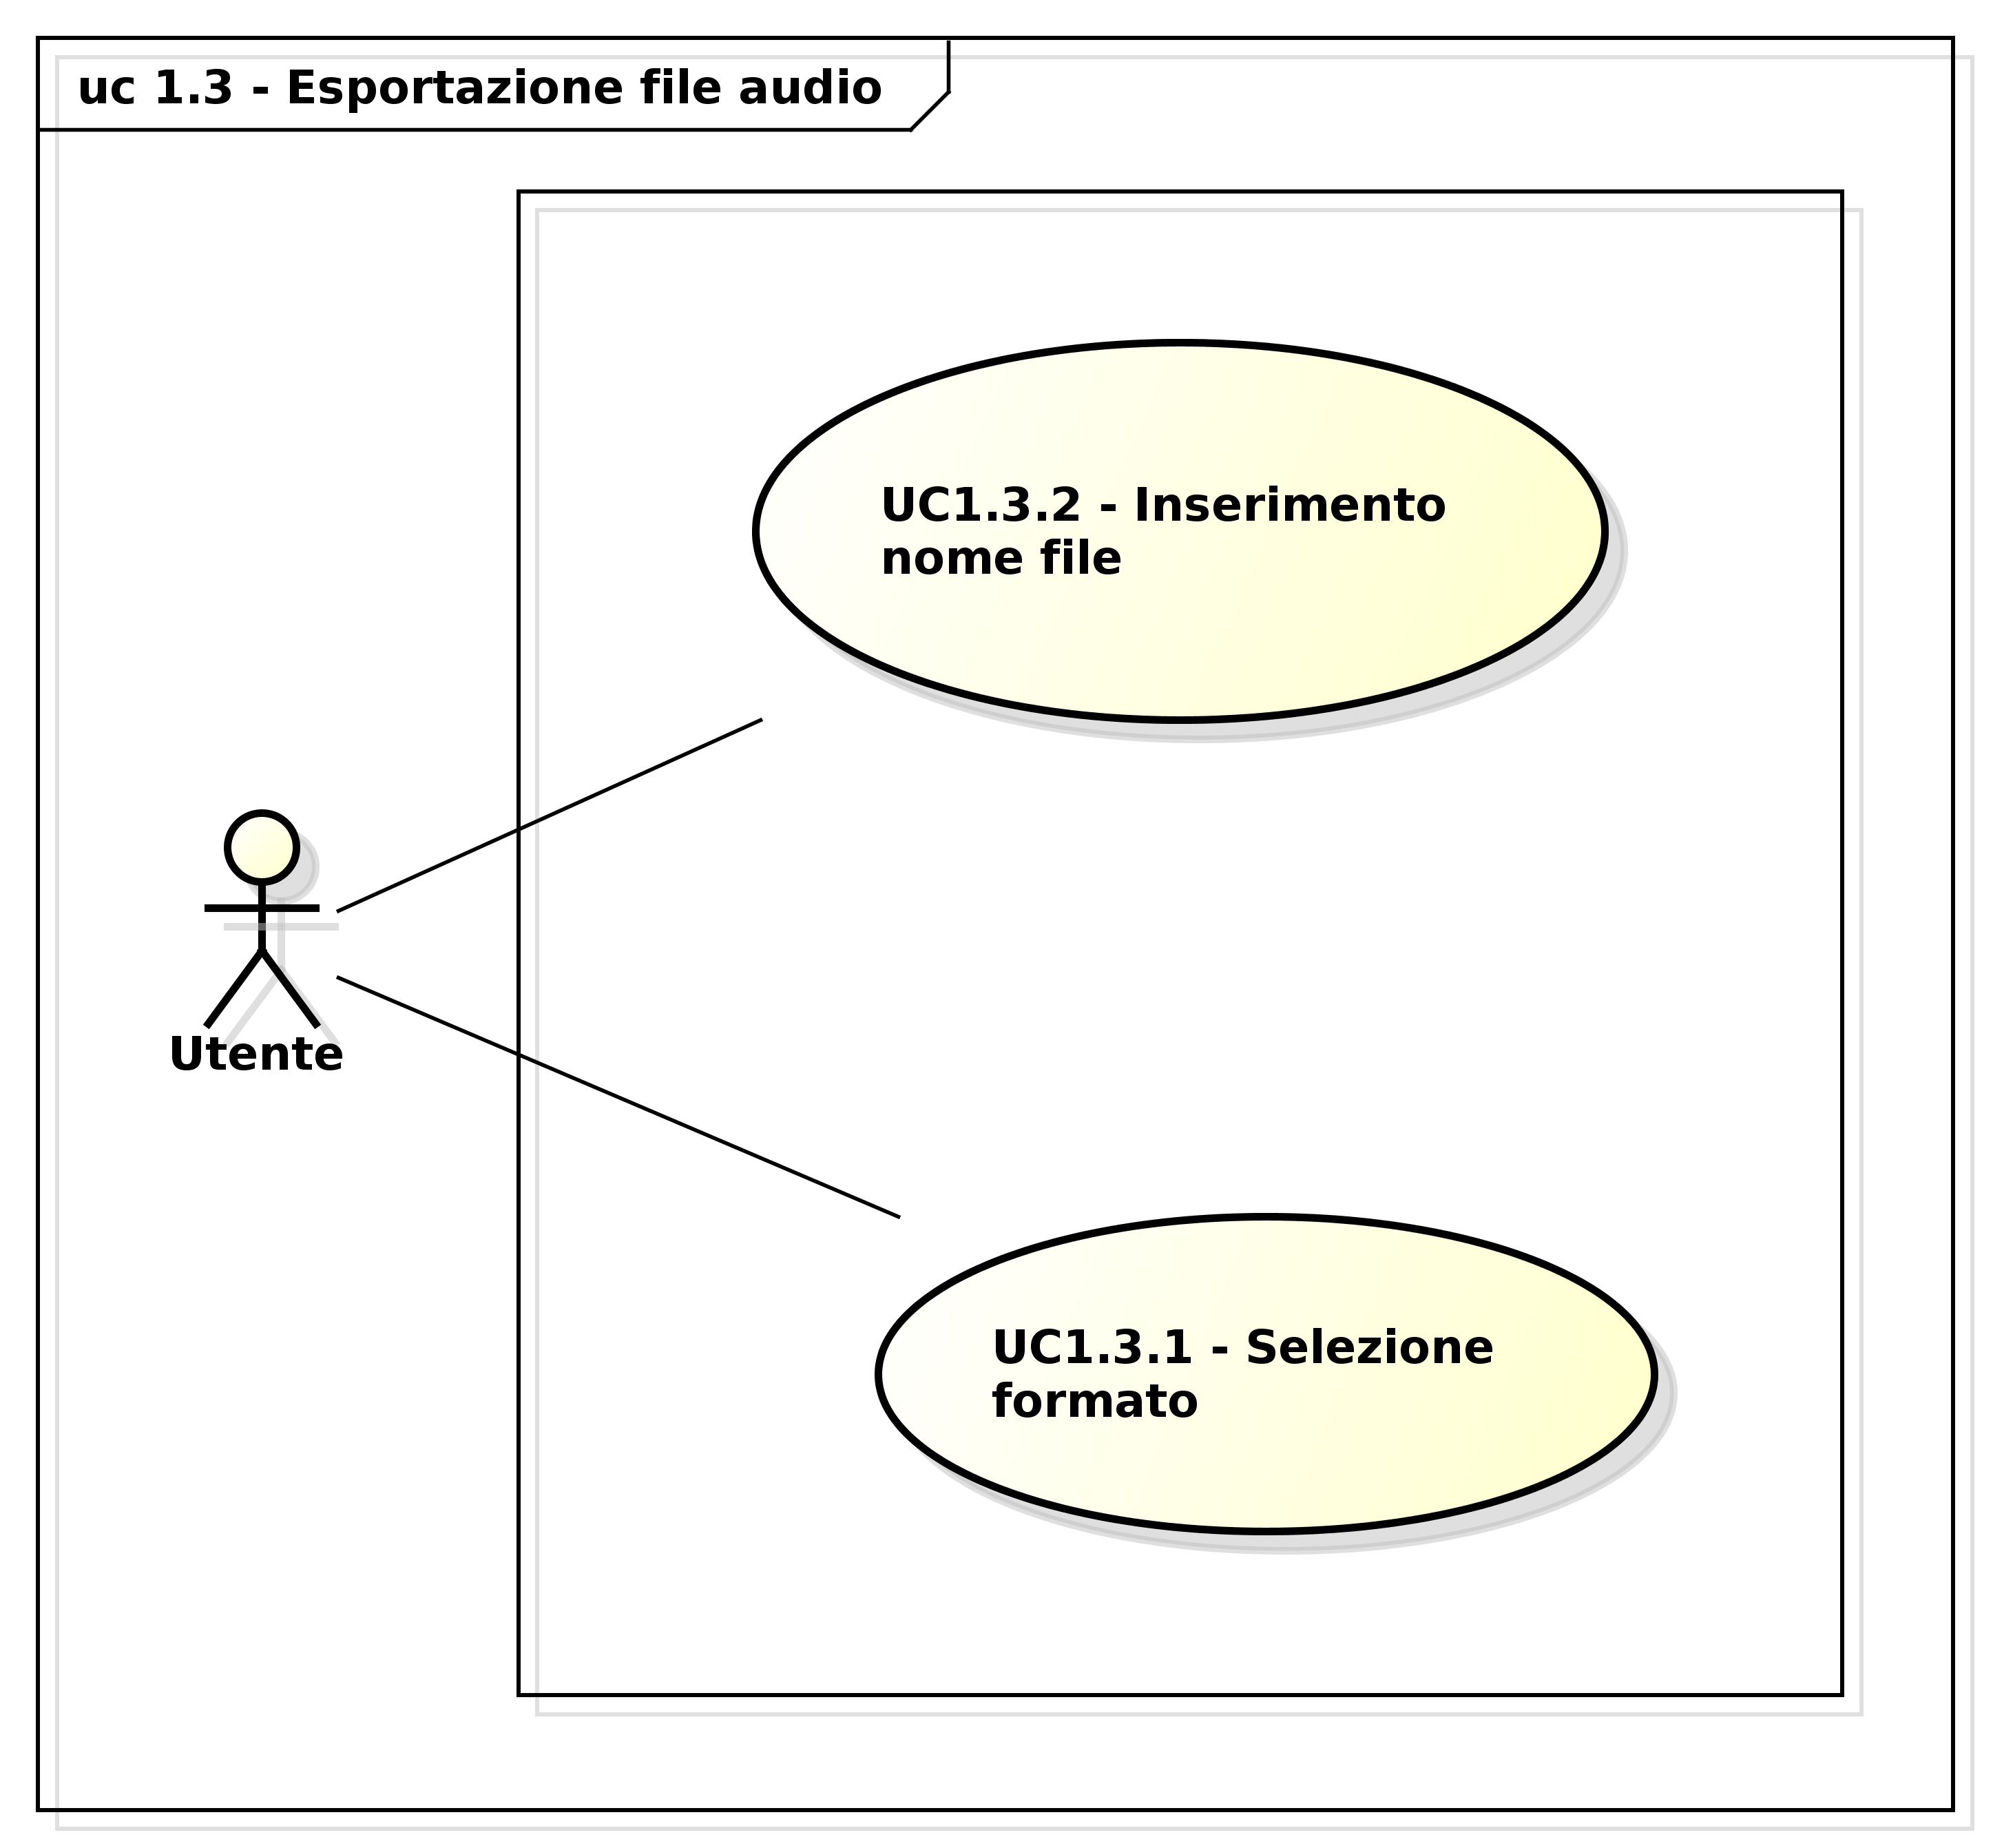
\includegraphics[scale=0.5]{UseCase_17_03_2016/immagini/uc_1_3_esportazione_audio_finale.png}
\captionsetup{labelfont=bf}
\caption{Caso d'uso UC1.3}
\end{figure}

\begin{itemize}
\item \textbf{Attore}: Utente;
\item \textbf{Scopo e descrizione}: l'utente digita il nome del file da generare e ne sceglie il formato di esportazione, 
\item \textbf{Precondizione}: il sistema è pronto ad esportare uno sceneggiato correttamente formato;
\item \textbf{Flusso principale degli eventi}:
\begin{enumerate}
\item L'utente digita il nome del file di esportazione (UC1.3.2);
\item L'utente seleziona il formato desiderato (UC1.3.1).
\end{enumerate}
\item \textbf{Scenari alternativi}: l'utente dcide di salvare il file con il nome di default; 
\item \textbf{Postcondizione}: viene effettuata l'esportazione nel formato desiderato.  
\end{itemize}

\subsection{Caso d'uso UC1.4: Salvataggio file}

\begin{figure}[htbp]
\centering
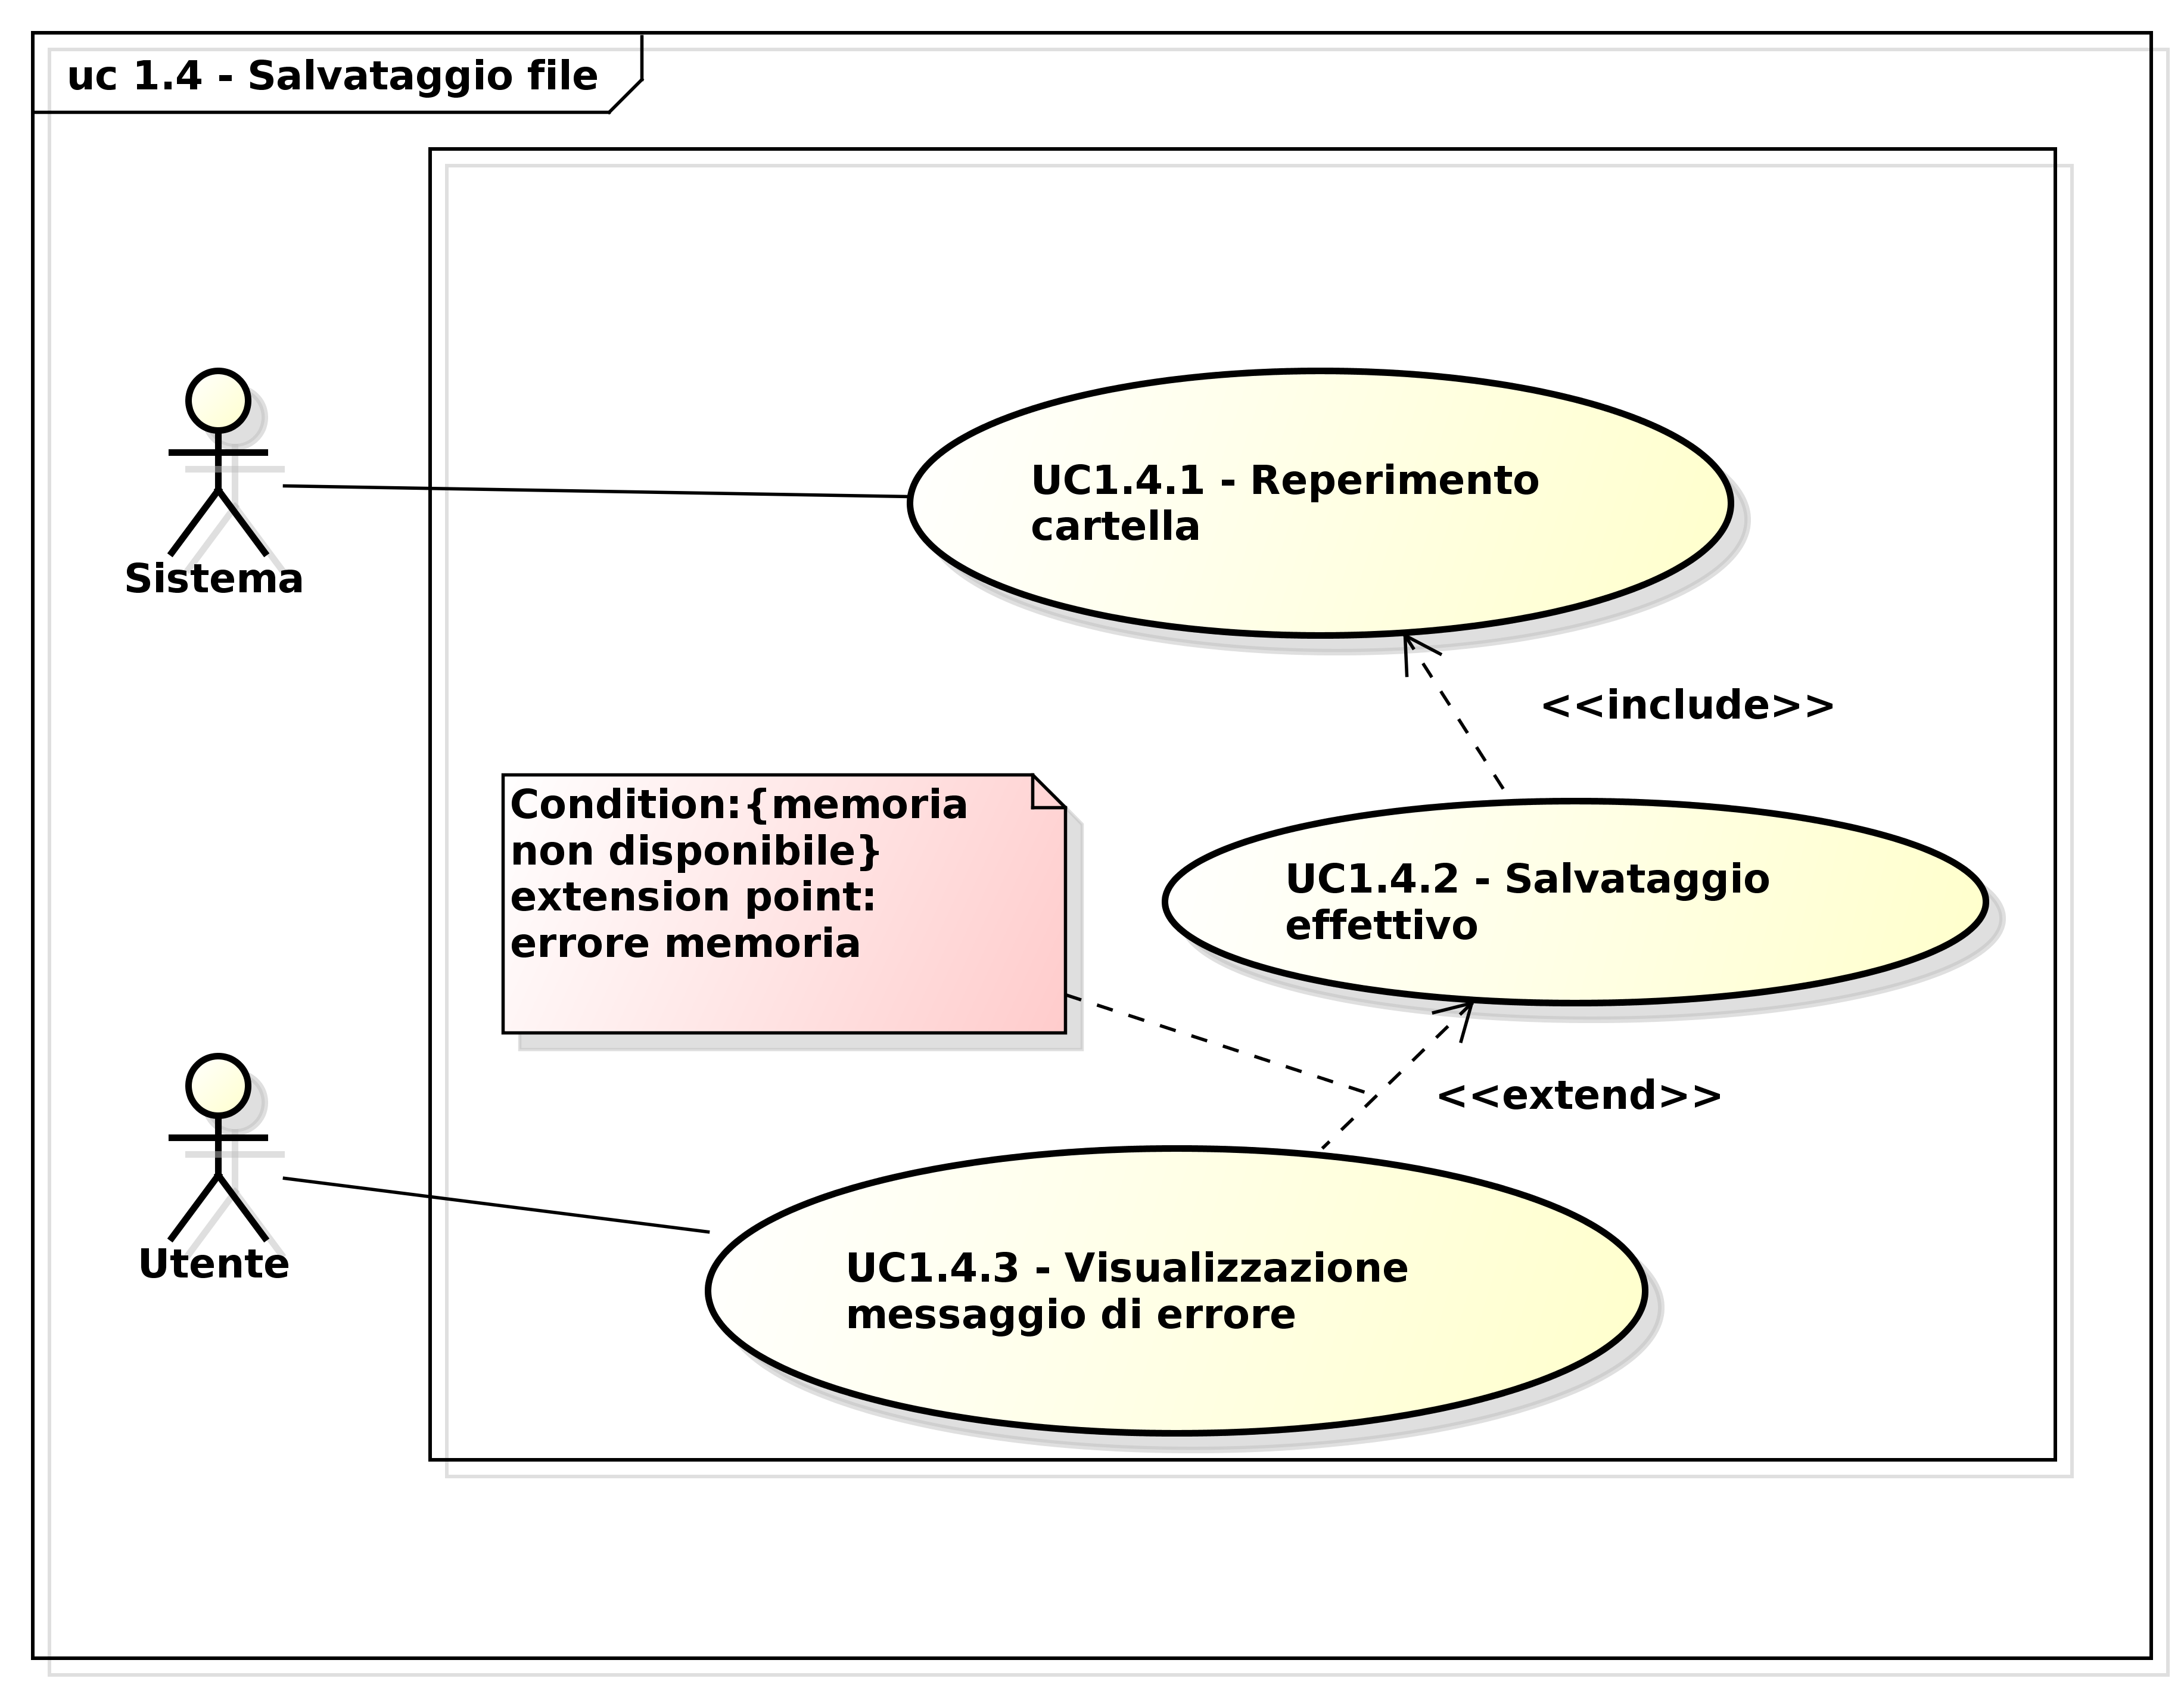
\includegraphics[scale=0.5]{UseCase_17_03_2016/immagini/uc_1_4_salvataggio_file.png}
\captionsetup{labelfont=bf}
\caption{Caso d'uso UC1.4}
\end{figure}

\begin{itemize}
\item \textbf{Attori}: Utente, Sistema;
\item \textbf{Scopo e descrizione}: l'utente può salvare le modifiche apportate ad uno sceneggiato; il Sistema provvederà al slavataggio effettivo reperendo la cartella di destinazione impostata di default;
\item \textbf{Precondizione}: il sistema è pronto ad effettuare il salvataggio;
\item \textbf{Flusso principale degli eventi}:
\begin{enumerate}
\item Il sistema reperisce la cartella di default (UC1.4.1);
\item Il sistema effettua il salvataggio (UC1.4.2).
\end{enumerate}
\item \textbf{Scenari alternativi}: il sistema avvertirà l'utente in caso il salvataggio non andasse a buon fine a causa di mancanza di memoria disponibile;  
\item \textbf{Postcondizione}: il salvataggio viene effettuato correttamente. 
\end{itemize}

\subsection{Caso d'uso UC1.7: Apertura file}

\begin{figure}[htbp]
\centering
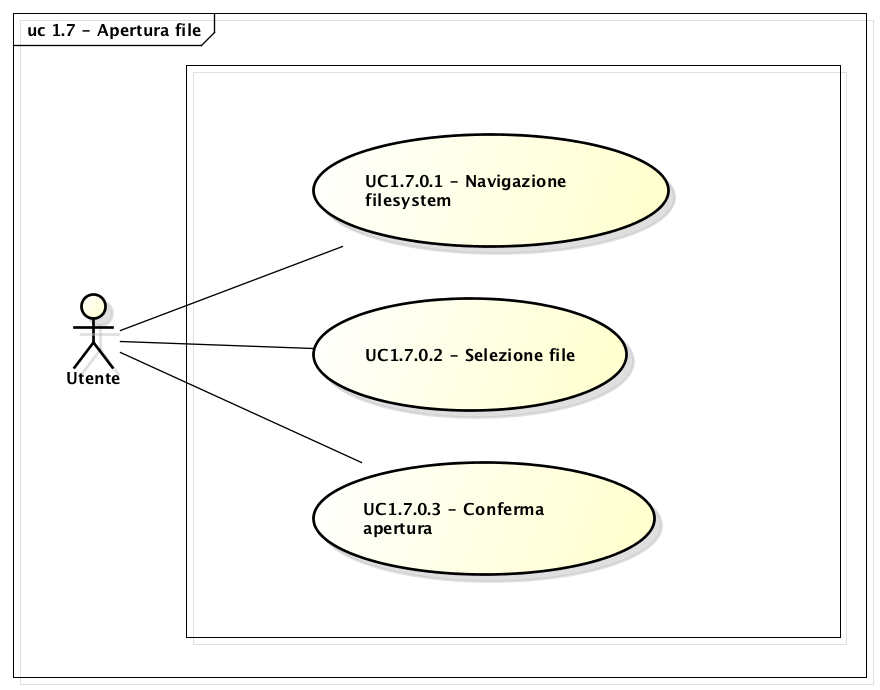
\includegraphics[scale=0.5]{UseCase_17_03_2016/immagini/uc_1_7_apertura_file.png}
\captionsetup{labelfont=bf}
\caption{Caso d'uso UC1.4}
\end{figure}

\begin{itemize}
\item \textbf{Attori}: Utente;
\item \textbf{Scopo e descrizione}: l'utente, navigando nel filesystem, può selezionare un file da aprire;
\item \textbf{Precondizione}: il programma è avviato;
\item \textbf{Flusso principale degli eventi}:
\begin{enumerate}
\item L'utente naviga nel filesystem (UC1.7.0.1);
\item L'utente seleziona il file da aprire (UC.1.7.0.2);
\item L'utente conferma l'apertura del file selezionato (UC1.7.0.3).
\end{enumerate}
\item \textbf{Scenari alternativi}: il file selezionato non è conforme alla tipologia di file necessario;
\item \textbf{Postcondizione}: il file viene aperto correttamente;
\end{itemize}

\subsection{Caso d'uso UC1.8: Modifica sceneggiato}

\begin{figure}[htbp]
\centering
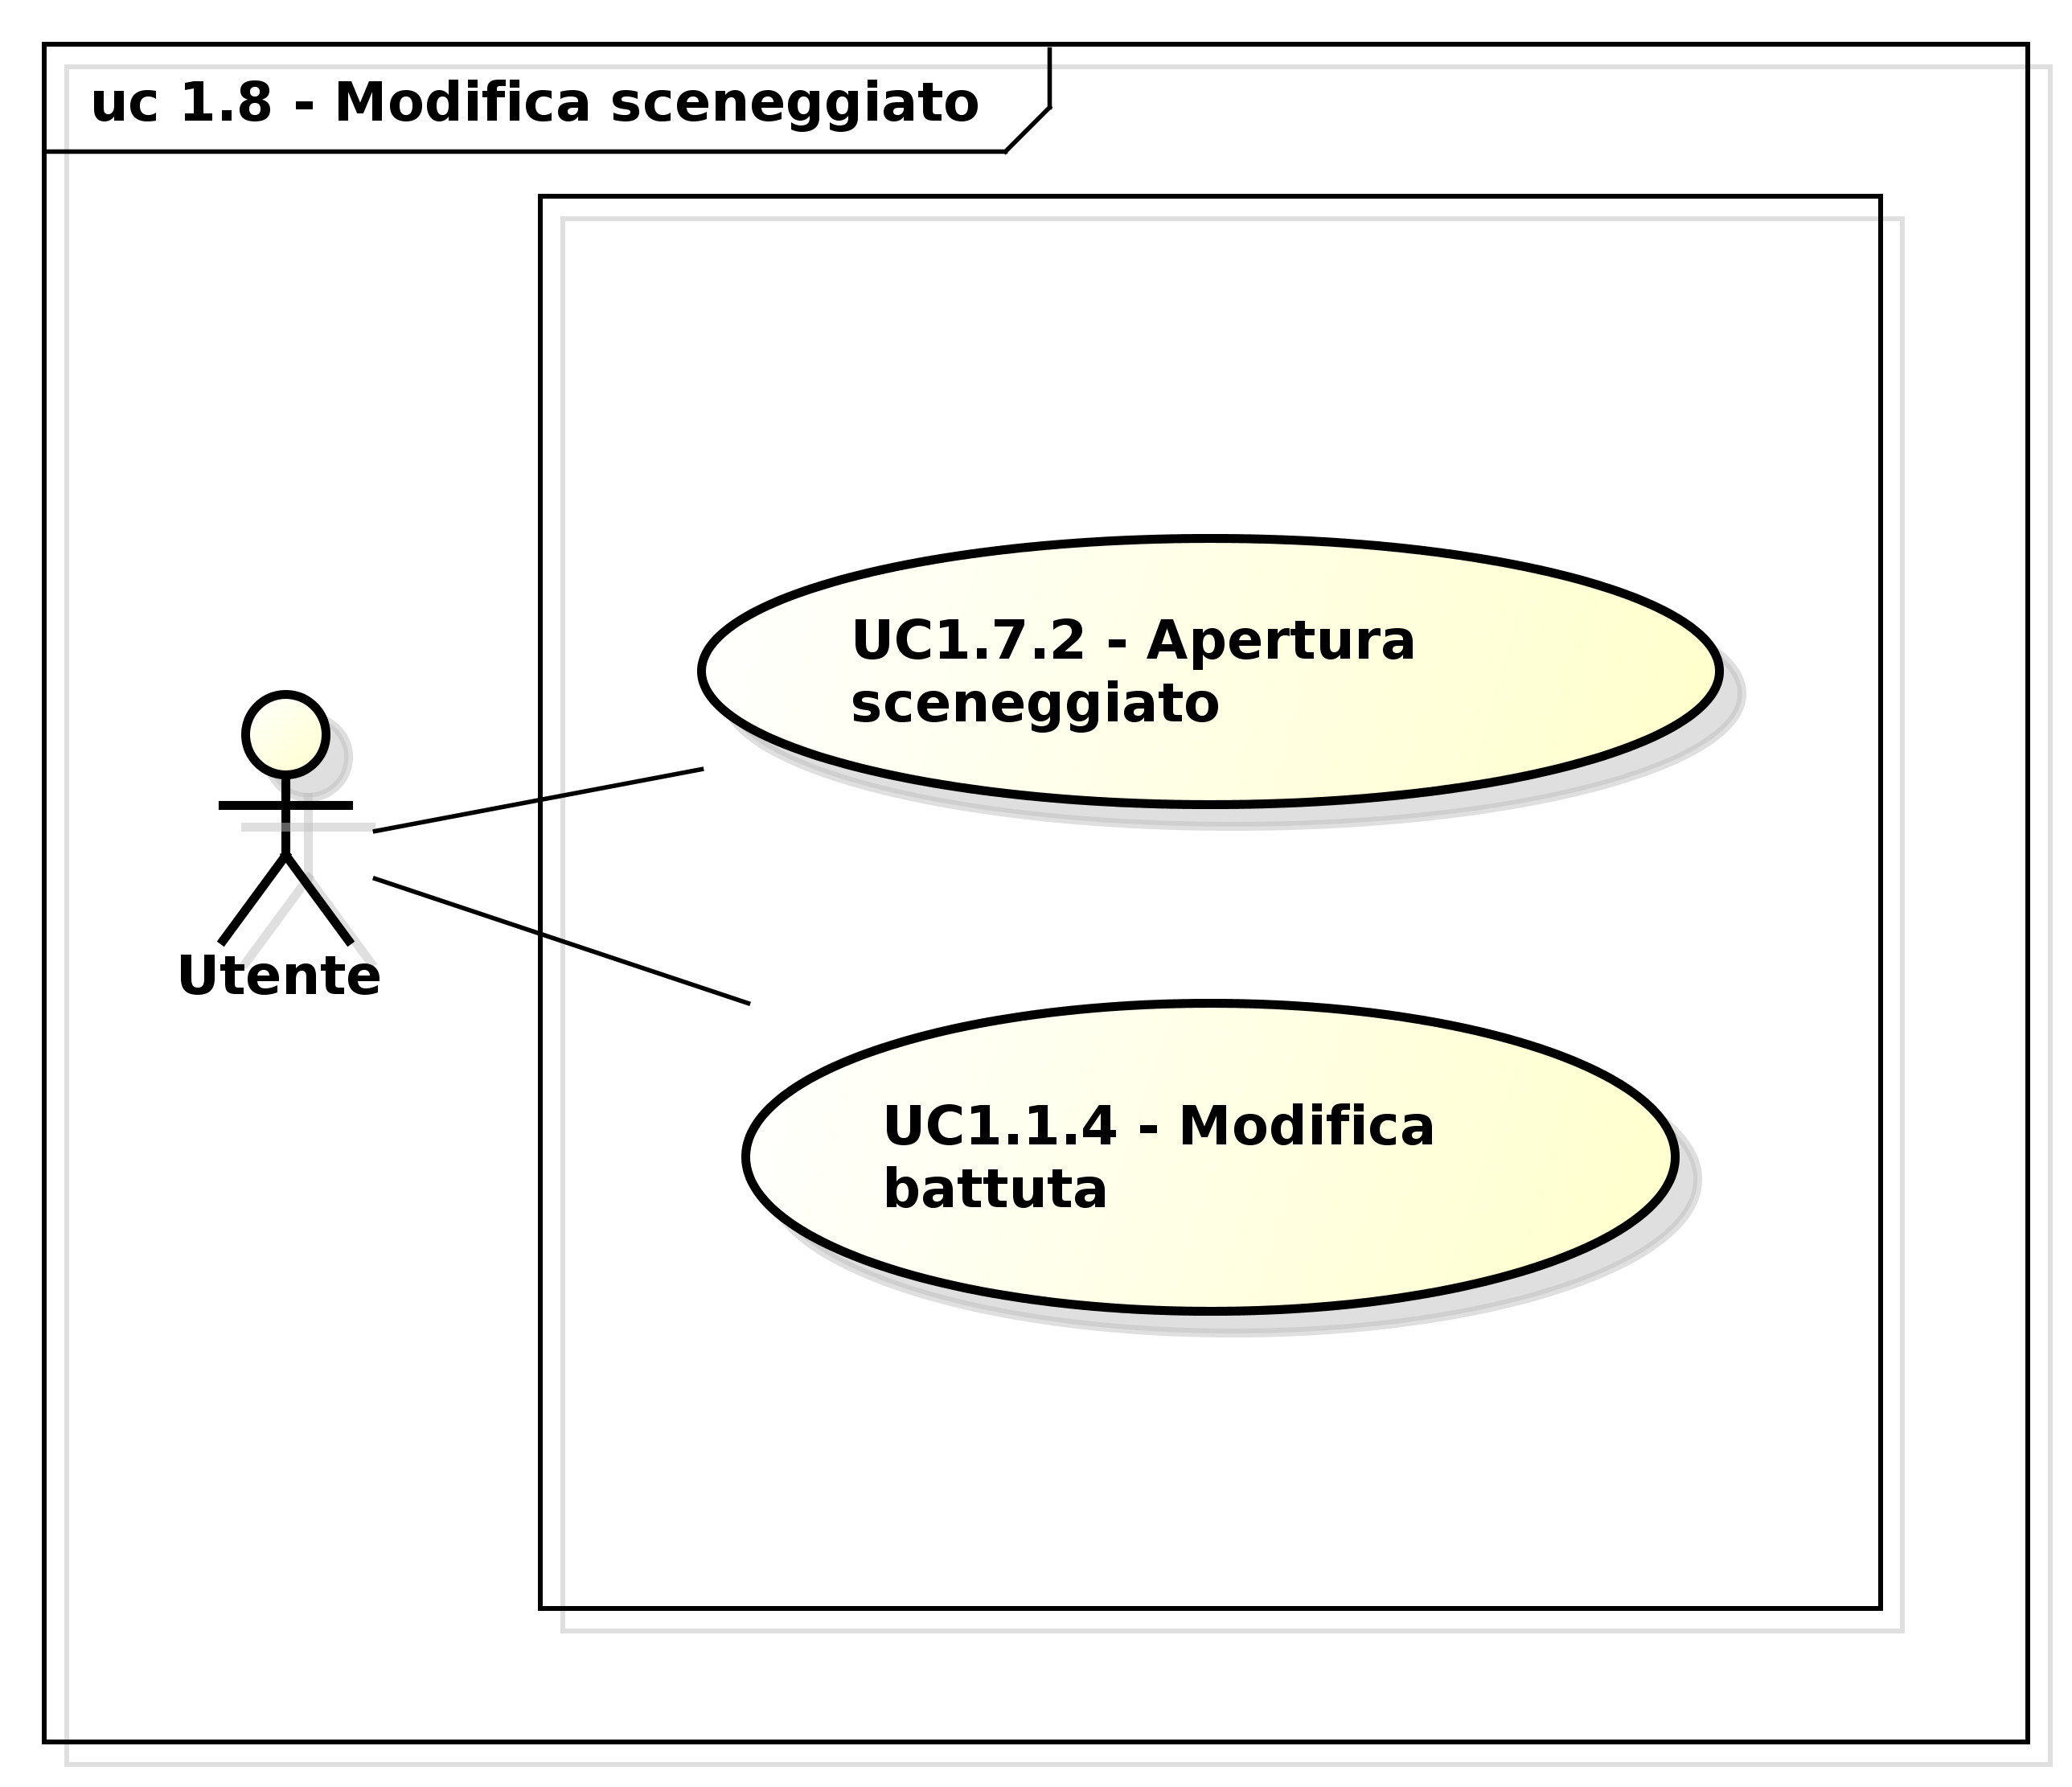
\includegraphics[scale=0.5]{UseCase_17_03_2016/immagini/uc_1_8_modifica_sceneggiato.png}
\captionsetup{labelfont=bf}
\caption{Caso d'uso UC1.8}
\end{figure}

\begin{itemize}
\item \textbf{Attori}: Utente;
\item \textbf{Scopo e descrizione}: l'utente può aprire uno sceneggiato già creato per modificarlo;
\item \textbf{Precondizione}: esiste almeno uno sceneggiato creato in precedenza;
\item \textbf{Flusso principale degli eventi}:
\begin{enumerate}
\item L'utente naviga nella lista degli sceneggiati già creati;
\item L'utente apre lo sceneggiato da modificare (UC1.7.2);
\item L'utente apporta le modifiche necessarie (UC1.1.4);
\end{enumerate}
\item \textbf{Scenari alternativi}: non esiste alcuno sceneggiato modificabile
\item \textbf{Postcondizione}: lo sceneggiato viene modificato correttamente.
\end{itemize}

\subsection{Caso d'uso UC2: Configurazione alto livello}

\begin{figure}[htbp]
\centering
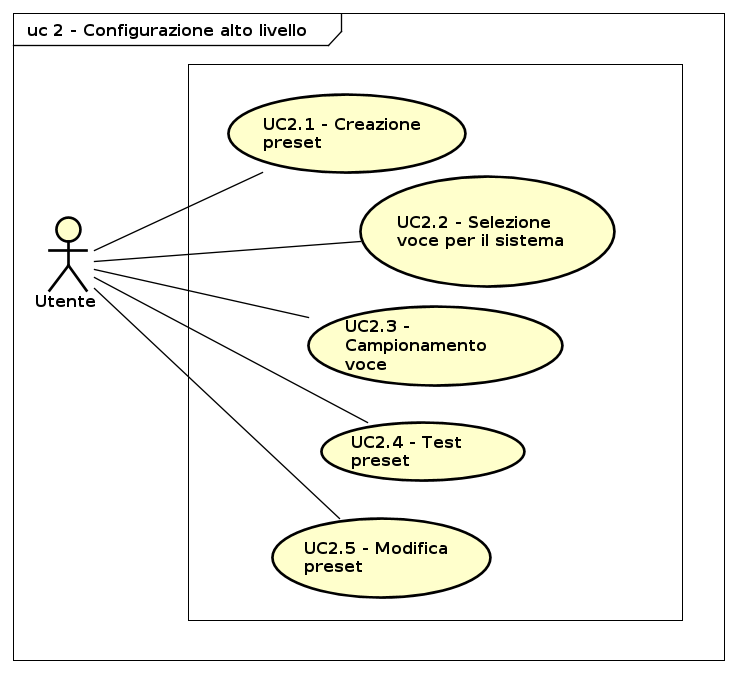
\includegraphics[scale=0.5]{UseCase_17_03_2016/immagini/uc_2_configurazione_alto_livello.png}
\captionsetup{labelfont=bf}
\caption{Caso d'uso UC2}
\end{figure}

\begin{itemize}
\item \textbf{Attori}: Utente;
\item \textbf{Scopo e descrizione}: dopo la corretta esecuzione della applicazione di configurazione, l'utente potrà creare dei nuovi preset, modificando parametri ed effetti; inoltre potrà selezionare una nuova voce da impostare per il sistema e anche campionare la sua voce;
\item \textbf{Precondizione}: l'applicazione è stata avviata correttamente;
\item \textbf{Flusso principale degli eventi}:
\begin{enumerate}
\item L'utente può creare un nuovo preset o modificarne uno già creato (UC2.1 - UC2.5);
\item L'utente può testare il preset creato (UC2.4); 
\item L'utente può selezionare una voce per il sistema (UC2.2);
\item L'utente può campionare la sua voce (UC2.3);
\end{enumerate}
\item \textbf{Postcondizione}: l'applicazione si aspetta direttive dall'utente.
\end{itemize}


\subsection{Caso d'uso UC2.1: Creazione preset}

\begin{figure}[htbp]
\centering
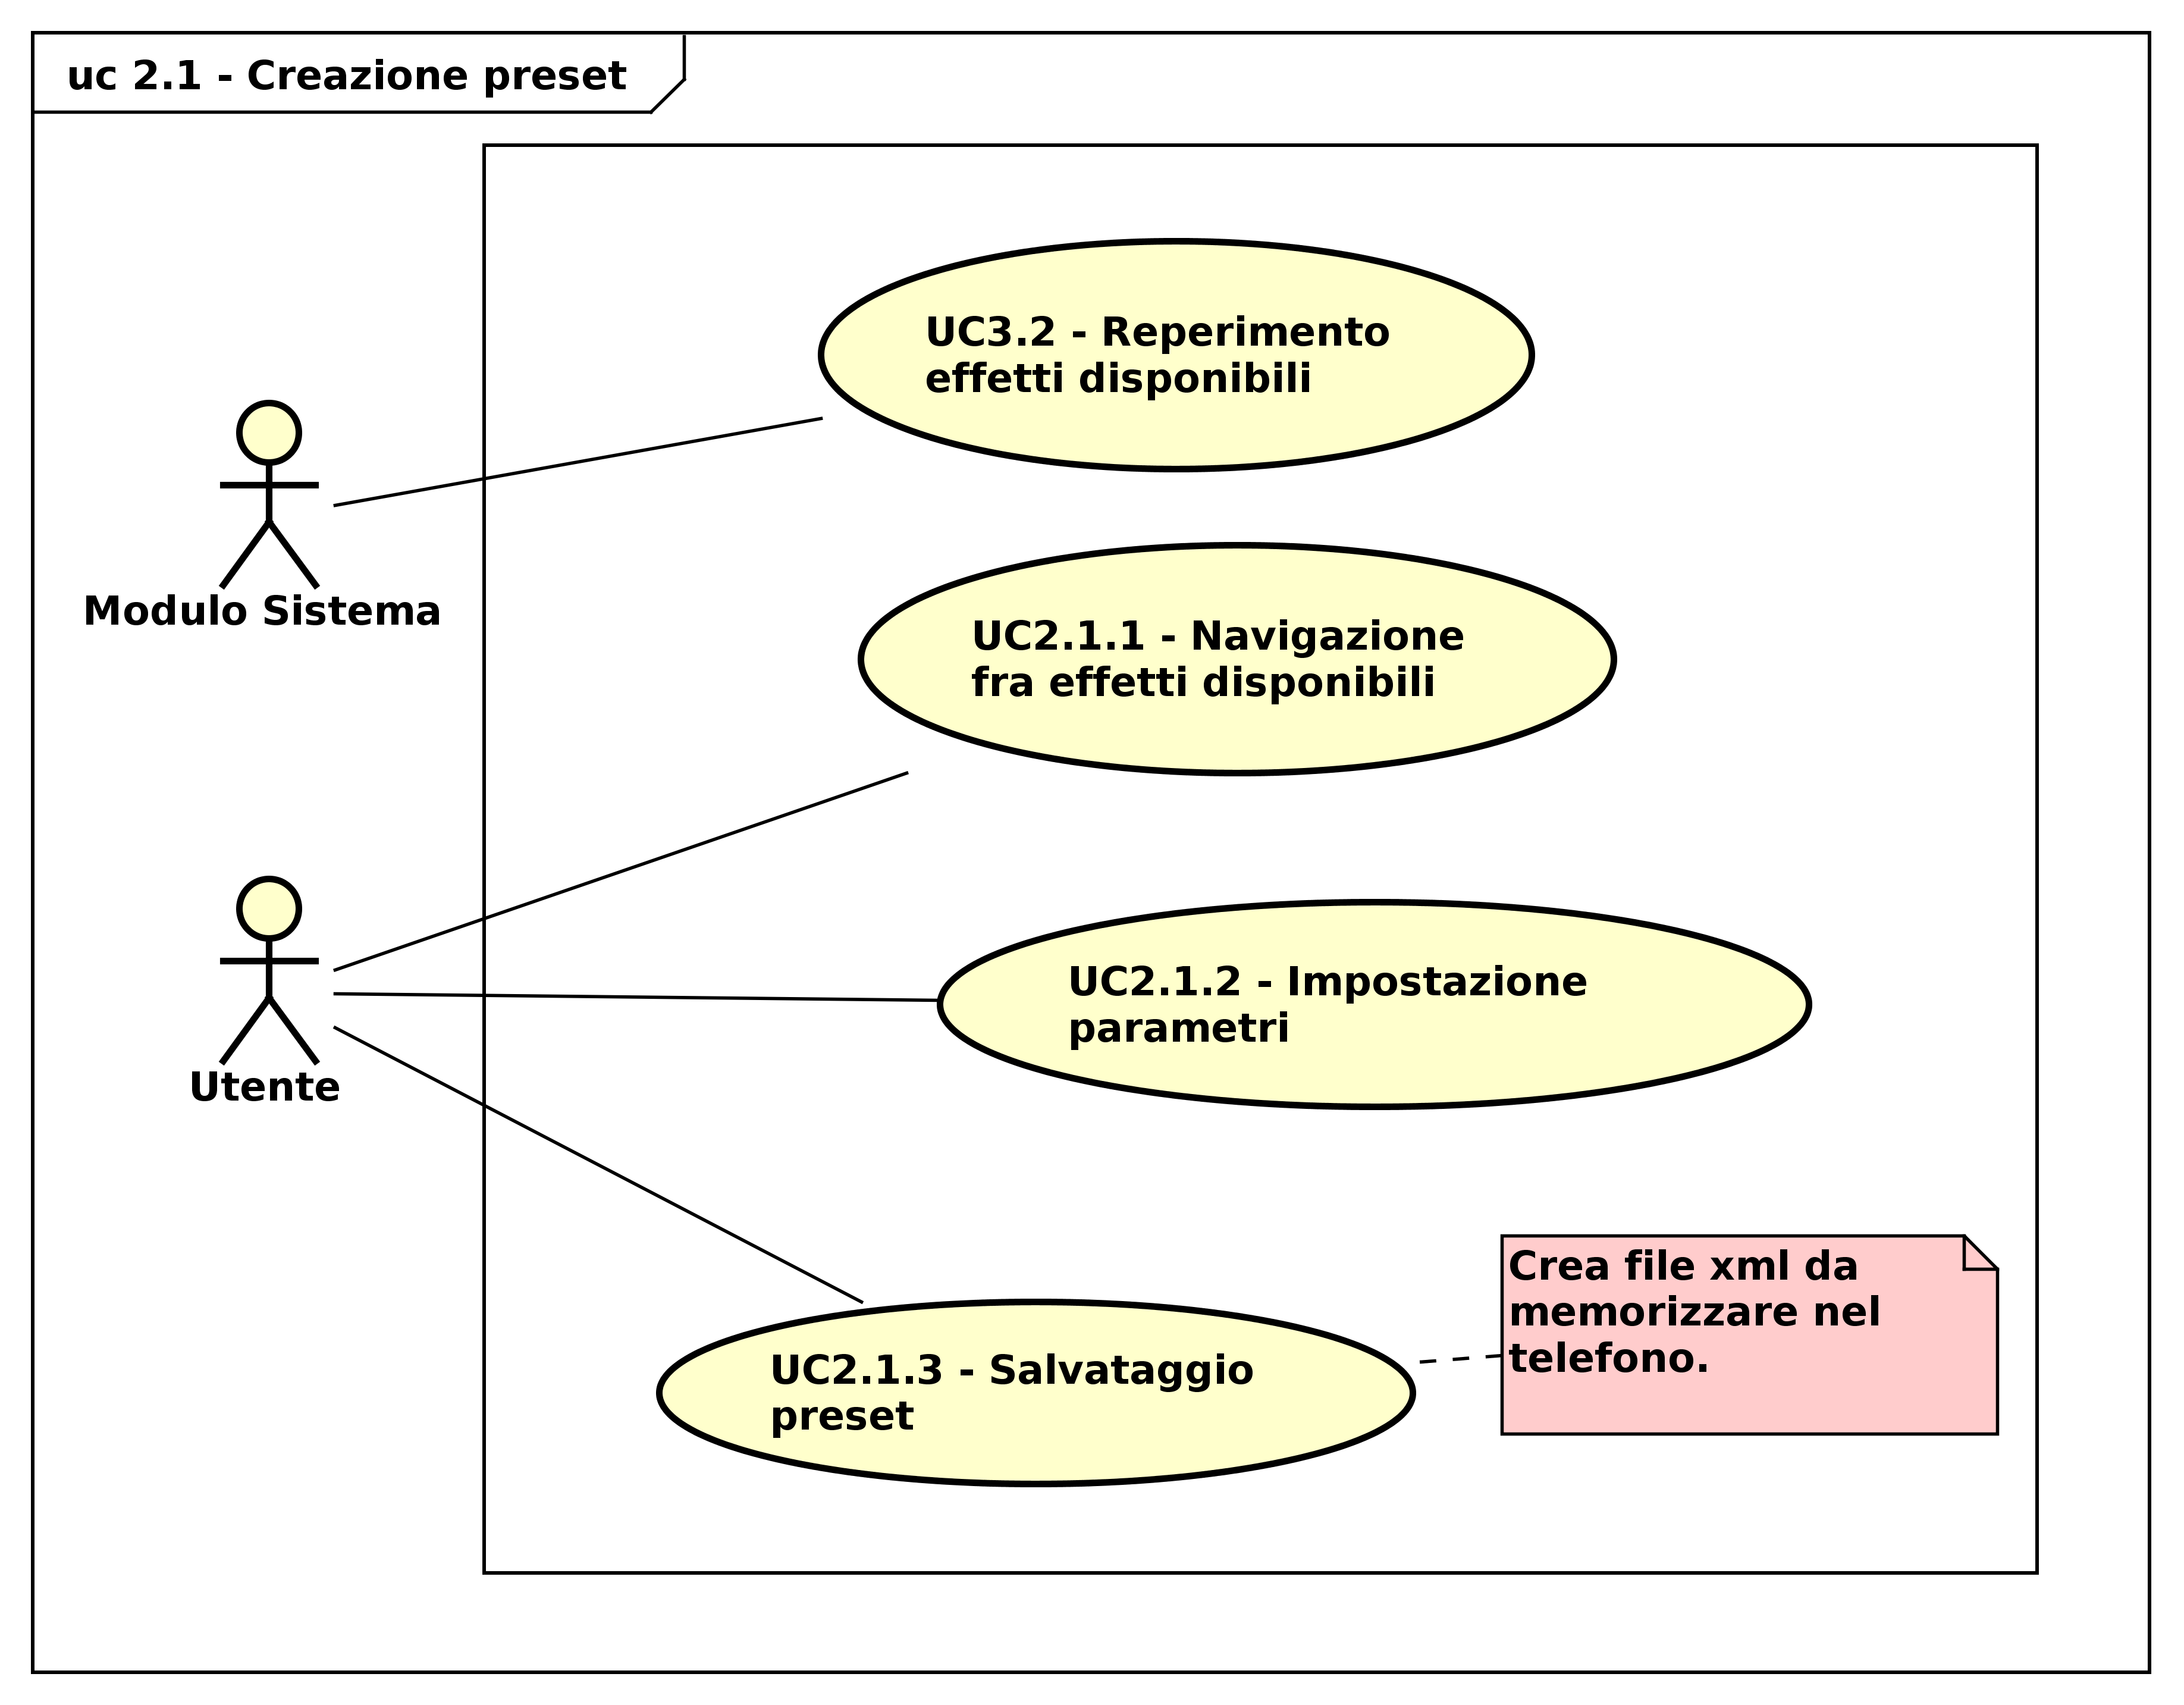
\includegraphics[scale=0.5]{UseCase_17_03_2016/immagini/uc_2_1_creazione_preset.png}
\captionsetup{labelfont=bf}
\caption{Caso d'uso UC2.1}
\end{figure}

\begin{itemize}
\item \textbf{Attori}: Utente, Modulo di sistema;
\item \textbf{Scopo e descrizione}: Dopo che il modulo di sistema ha reperito gli effetti disponibili, l'utente potrà navigare tra questi ultimi, selezionarli e associarli a voci; potrà in fine salvare i cambiamenti apportati;
\item \textbf{Precondizione}: il sistema ha reperito gli effetti disponibili;
\item \textbf{Flusso principale degli eventi}:
\begin{enumerate}
\item Il modulo reperisce gli effetti (UC3.2);
\item L'utente può navigare tra gli effetti disponibili reperiti (UC2.1.1);
\item L'utente può settare dei parametri (UC2.1.2);
\item L'utente può salvare il preset creato.
\end{enumerate}
\item \textbf{Postcondizione}: è stato salvato un preset creato dall'utente.
\end{itemize}

\subsection{Caso d'uso UC2.2: Selezione voce per il sistema}

\begin{figure}[htbp]
\centering
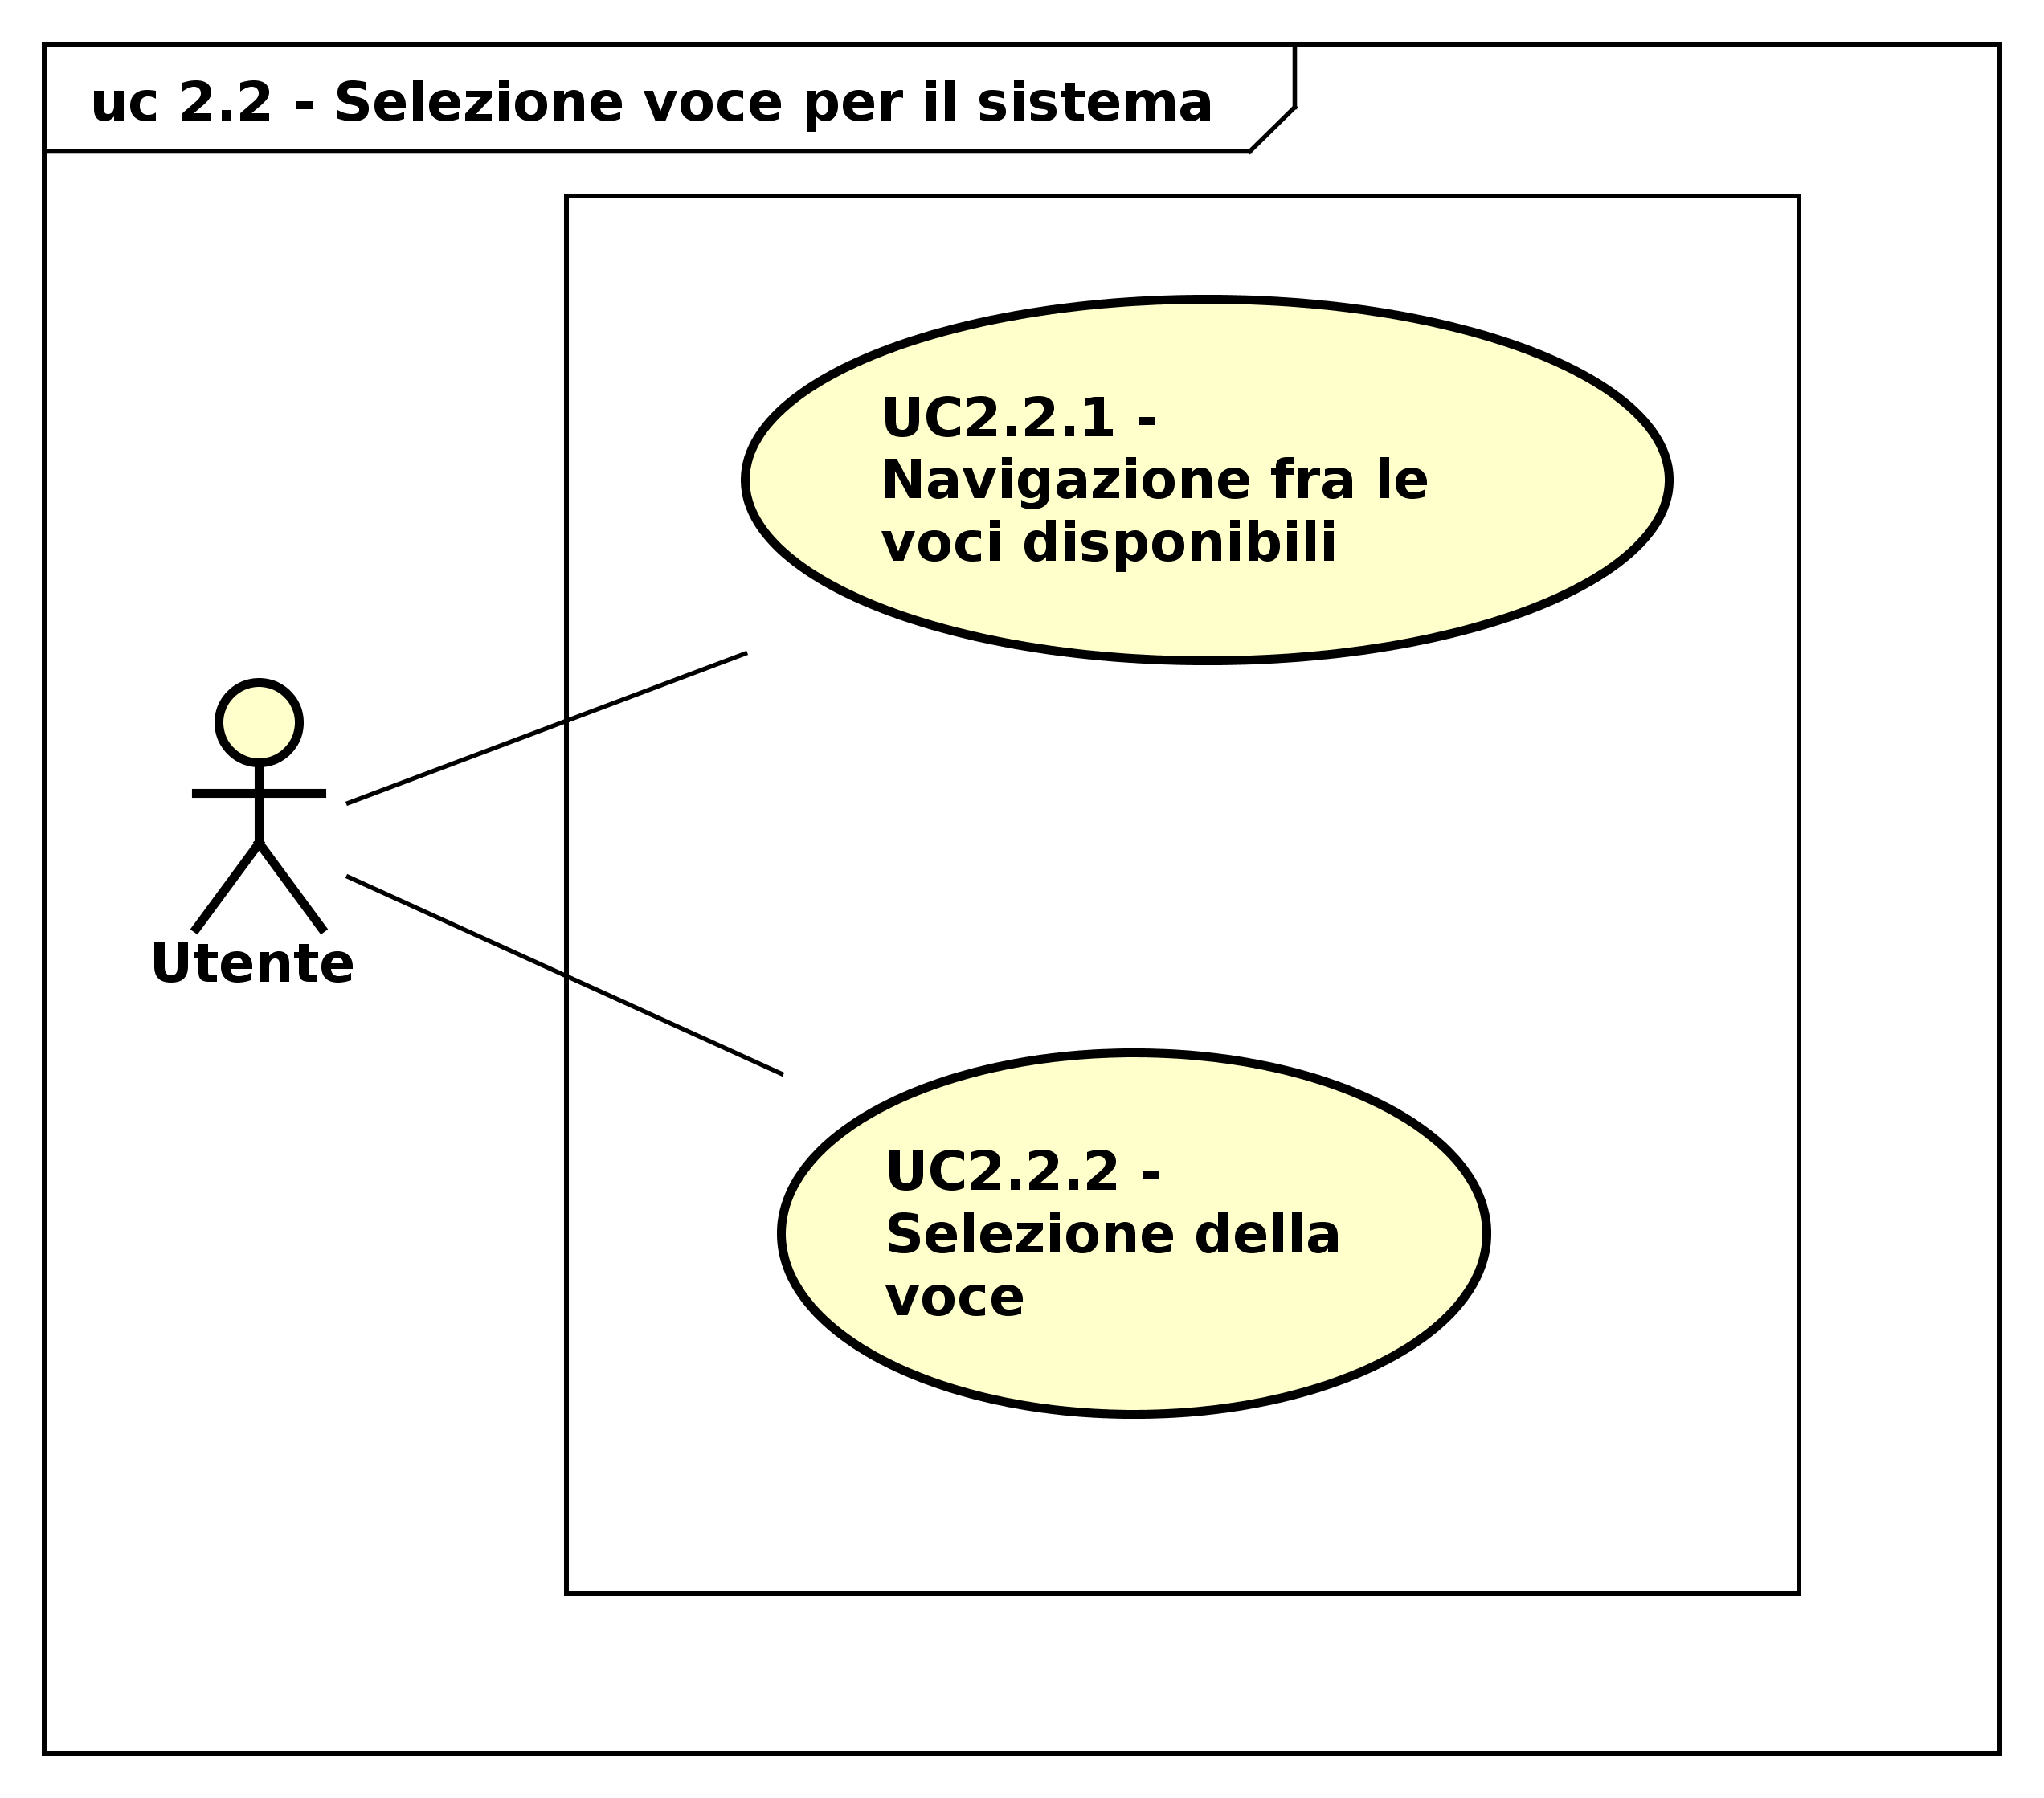
\includegraphics[scale=0.5]{UseCase_17_03_2016/immagini/uc_2_2_selezione_voce_sistema.png}
\captionsetup{labelfont=bf}
\caption{Caso d'uso UC2.2}
\end{figure}

\begin{itemize}
\item \textbf{Attori}: Utente;
\item \textbf{Scopo e descrizione}: l'utente può impostare una delle voci disponibili come voce di default per il sistema;
\item \textbf{Precondizione}: esistono voci disponibili;
\item \textbf{Postcondizione}: la voce è stata associata correttamente.
\end{itemize}

\subsection{Caso d'uso UC2.3: Campionamento voce}

\begin{figure}[htbp]
\centering
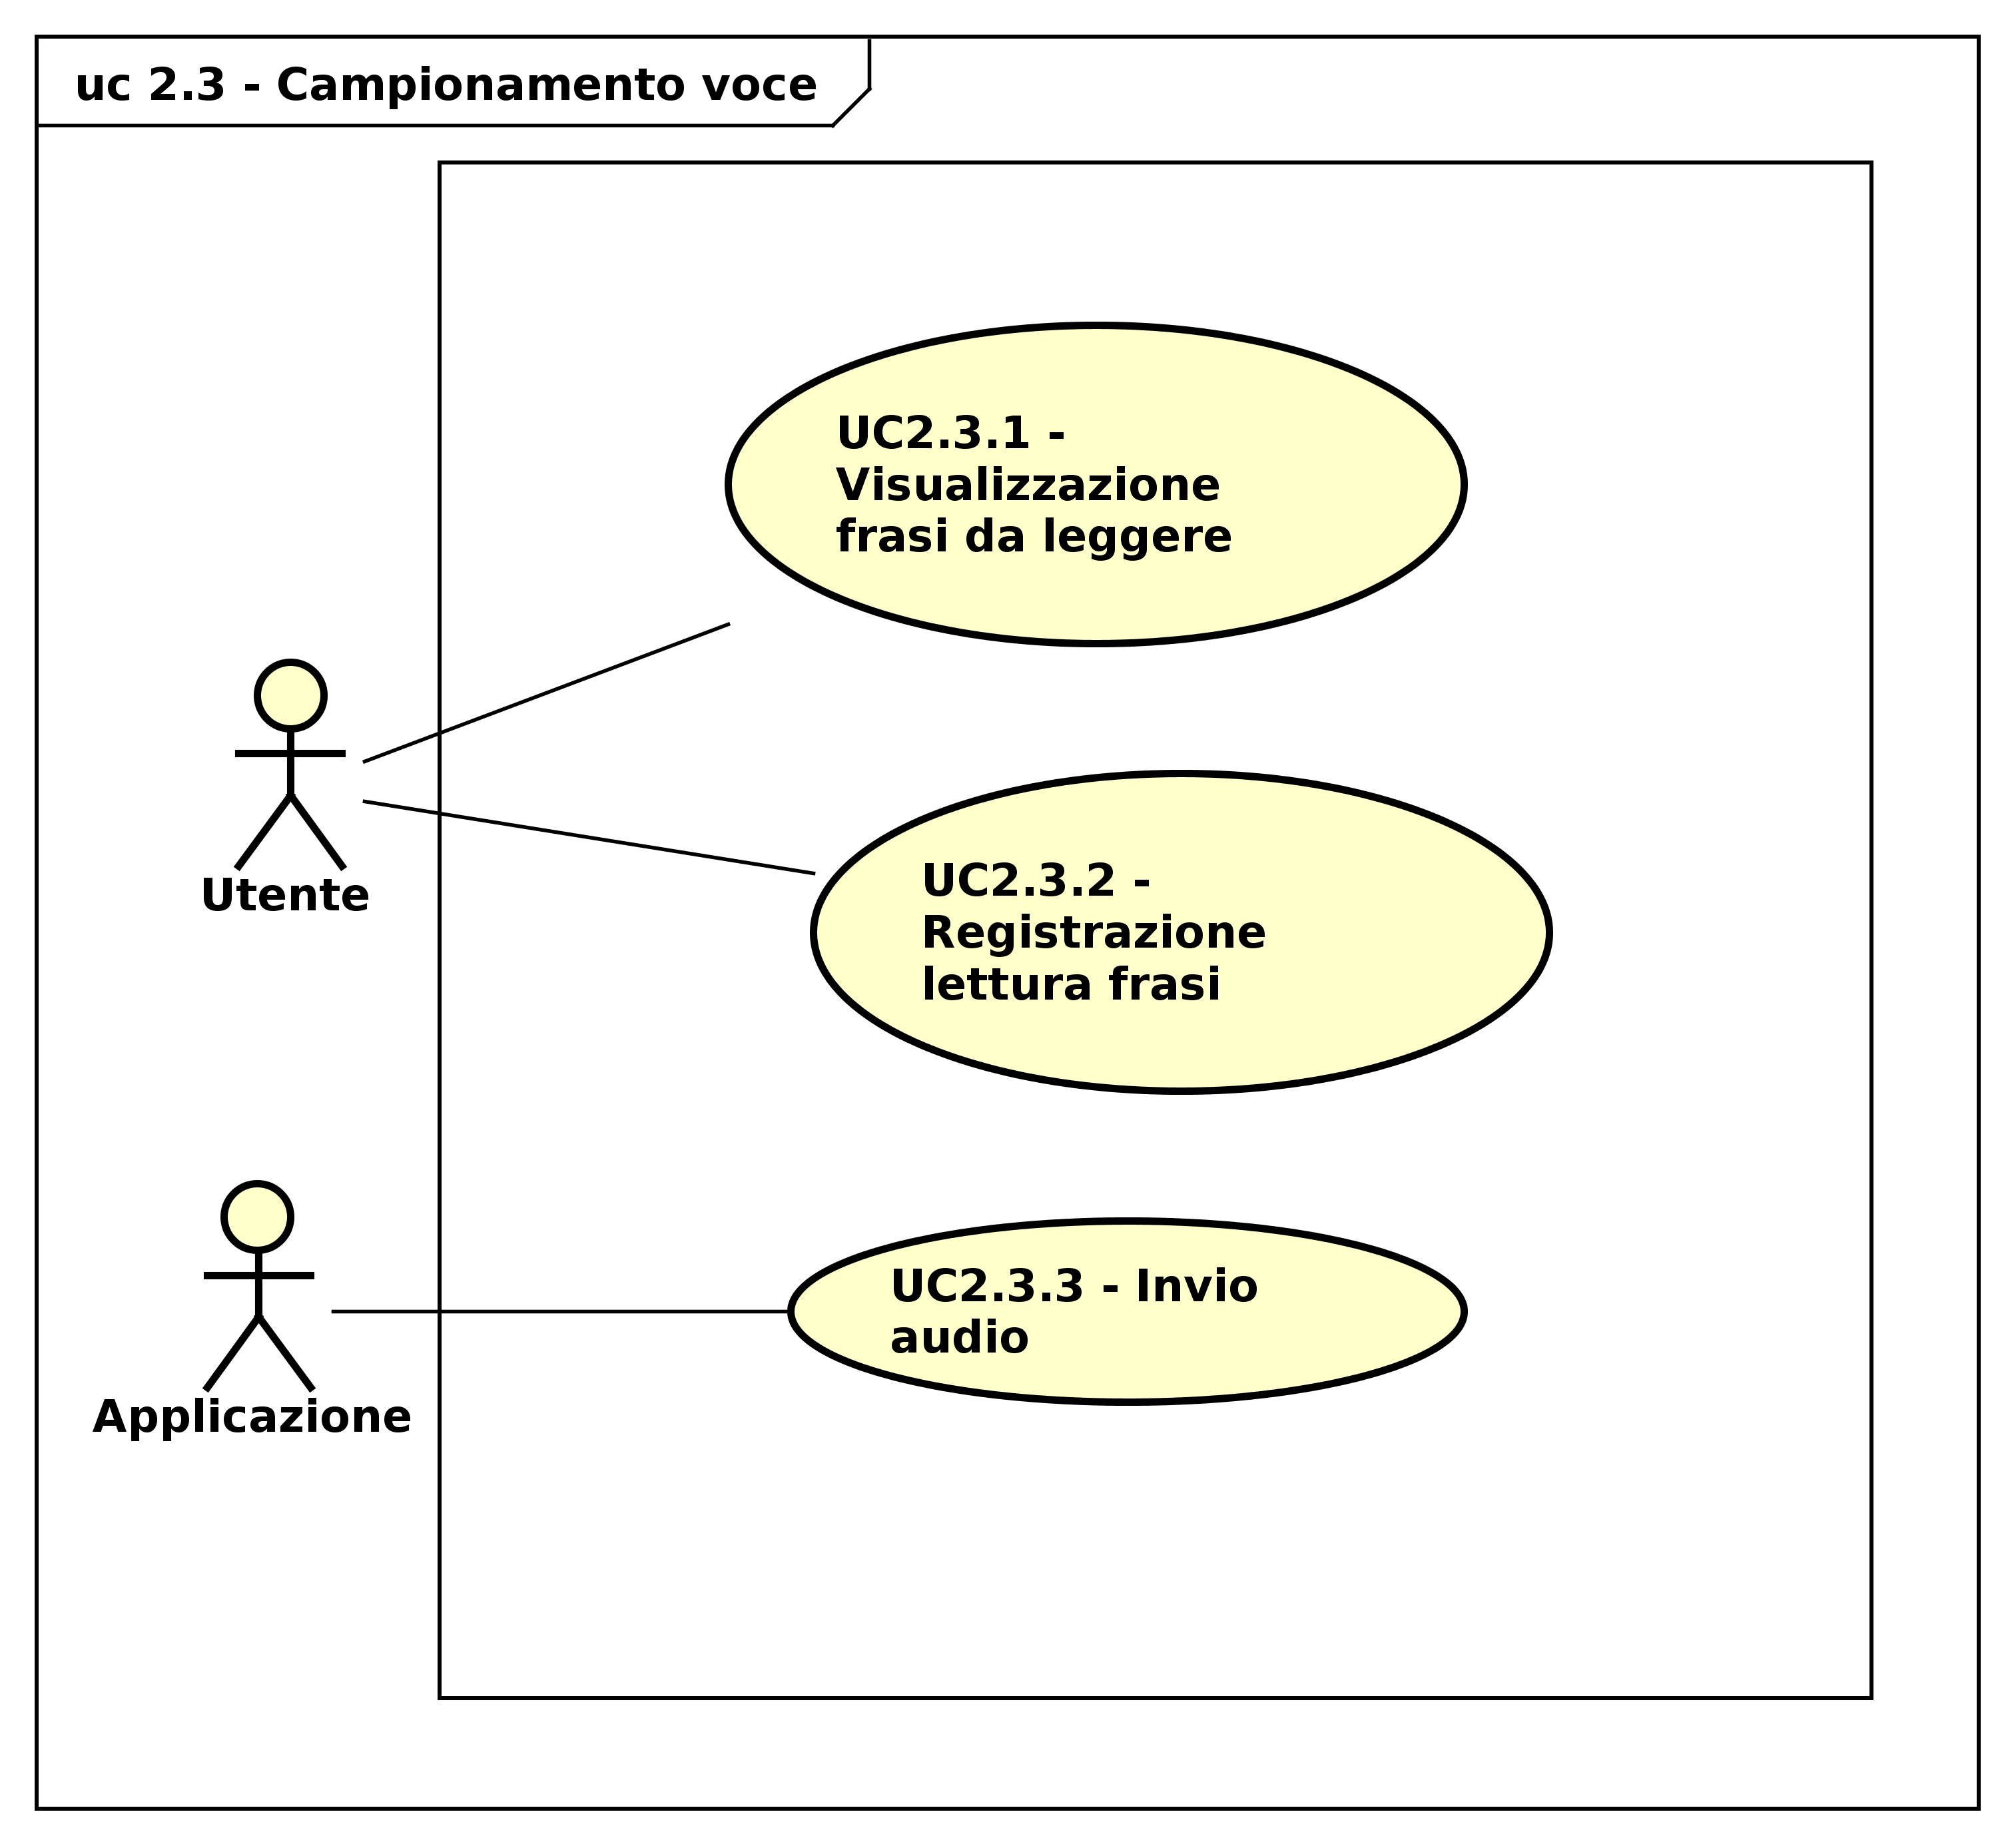
\includegraphics[scale=0.5]{UseCase_17_03_2016/immagini/uc_2_3_campionamento_voce.png}
\captionsetup{labelfont=bf}
\caption{Caso d'uso UC2.3}
\end{figure}

\begin{itemize}
\item \textbf{Attori}: Utente, Applicazione;
\item \textbf{Scopo e descrizione}: l'utente può campionare la sua voce  eseguendo una procedura di lettura e registrazione di frasi che verranno inviate al server dall'applicazione;
\item \textbf{Precondizione}: il sistema è pronto per il campionamento;
\item \textbf{Flusso principale degli eventi}:
\begin{enumerate}
\item L'utente visualizza la frase da leggere (UC2.3.1);
\item L'utente legge la frase che viene registrata (UC2.3.2);
\item L'applicazione invia la registrazione al server per il campionamento, per poi ricominciare dal punto 1 mostrando all'utente una nuova frase da leggere (UC2.3.3);
\end{enumerate}
\item \textbf{Postcondizione}: il campionamento è andato a buon fine.
\end{itemize}

\subsection{Caso d'uso UC2.4: Test preset}

\begin{figure}[htbp]
\centering
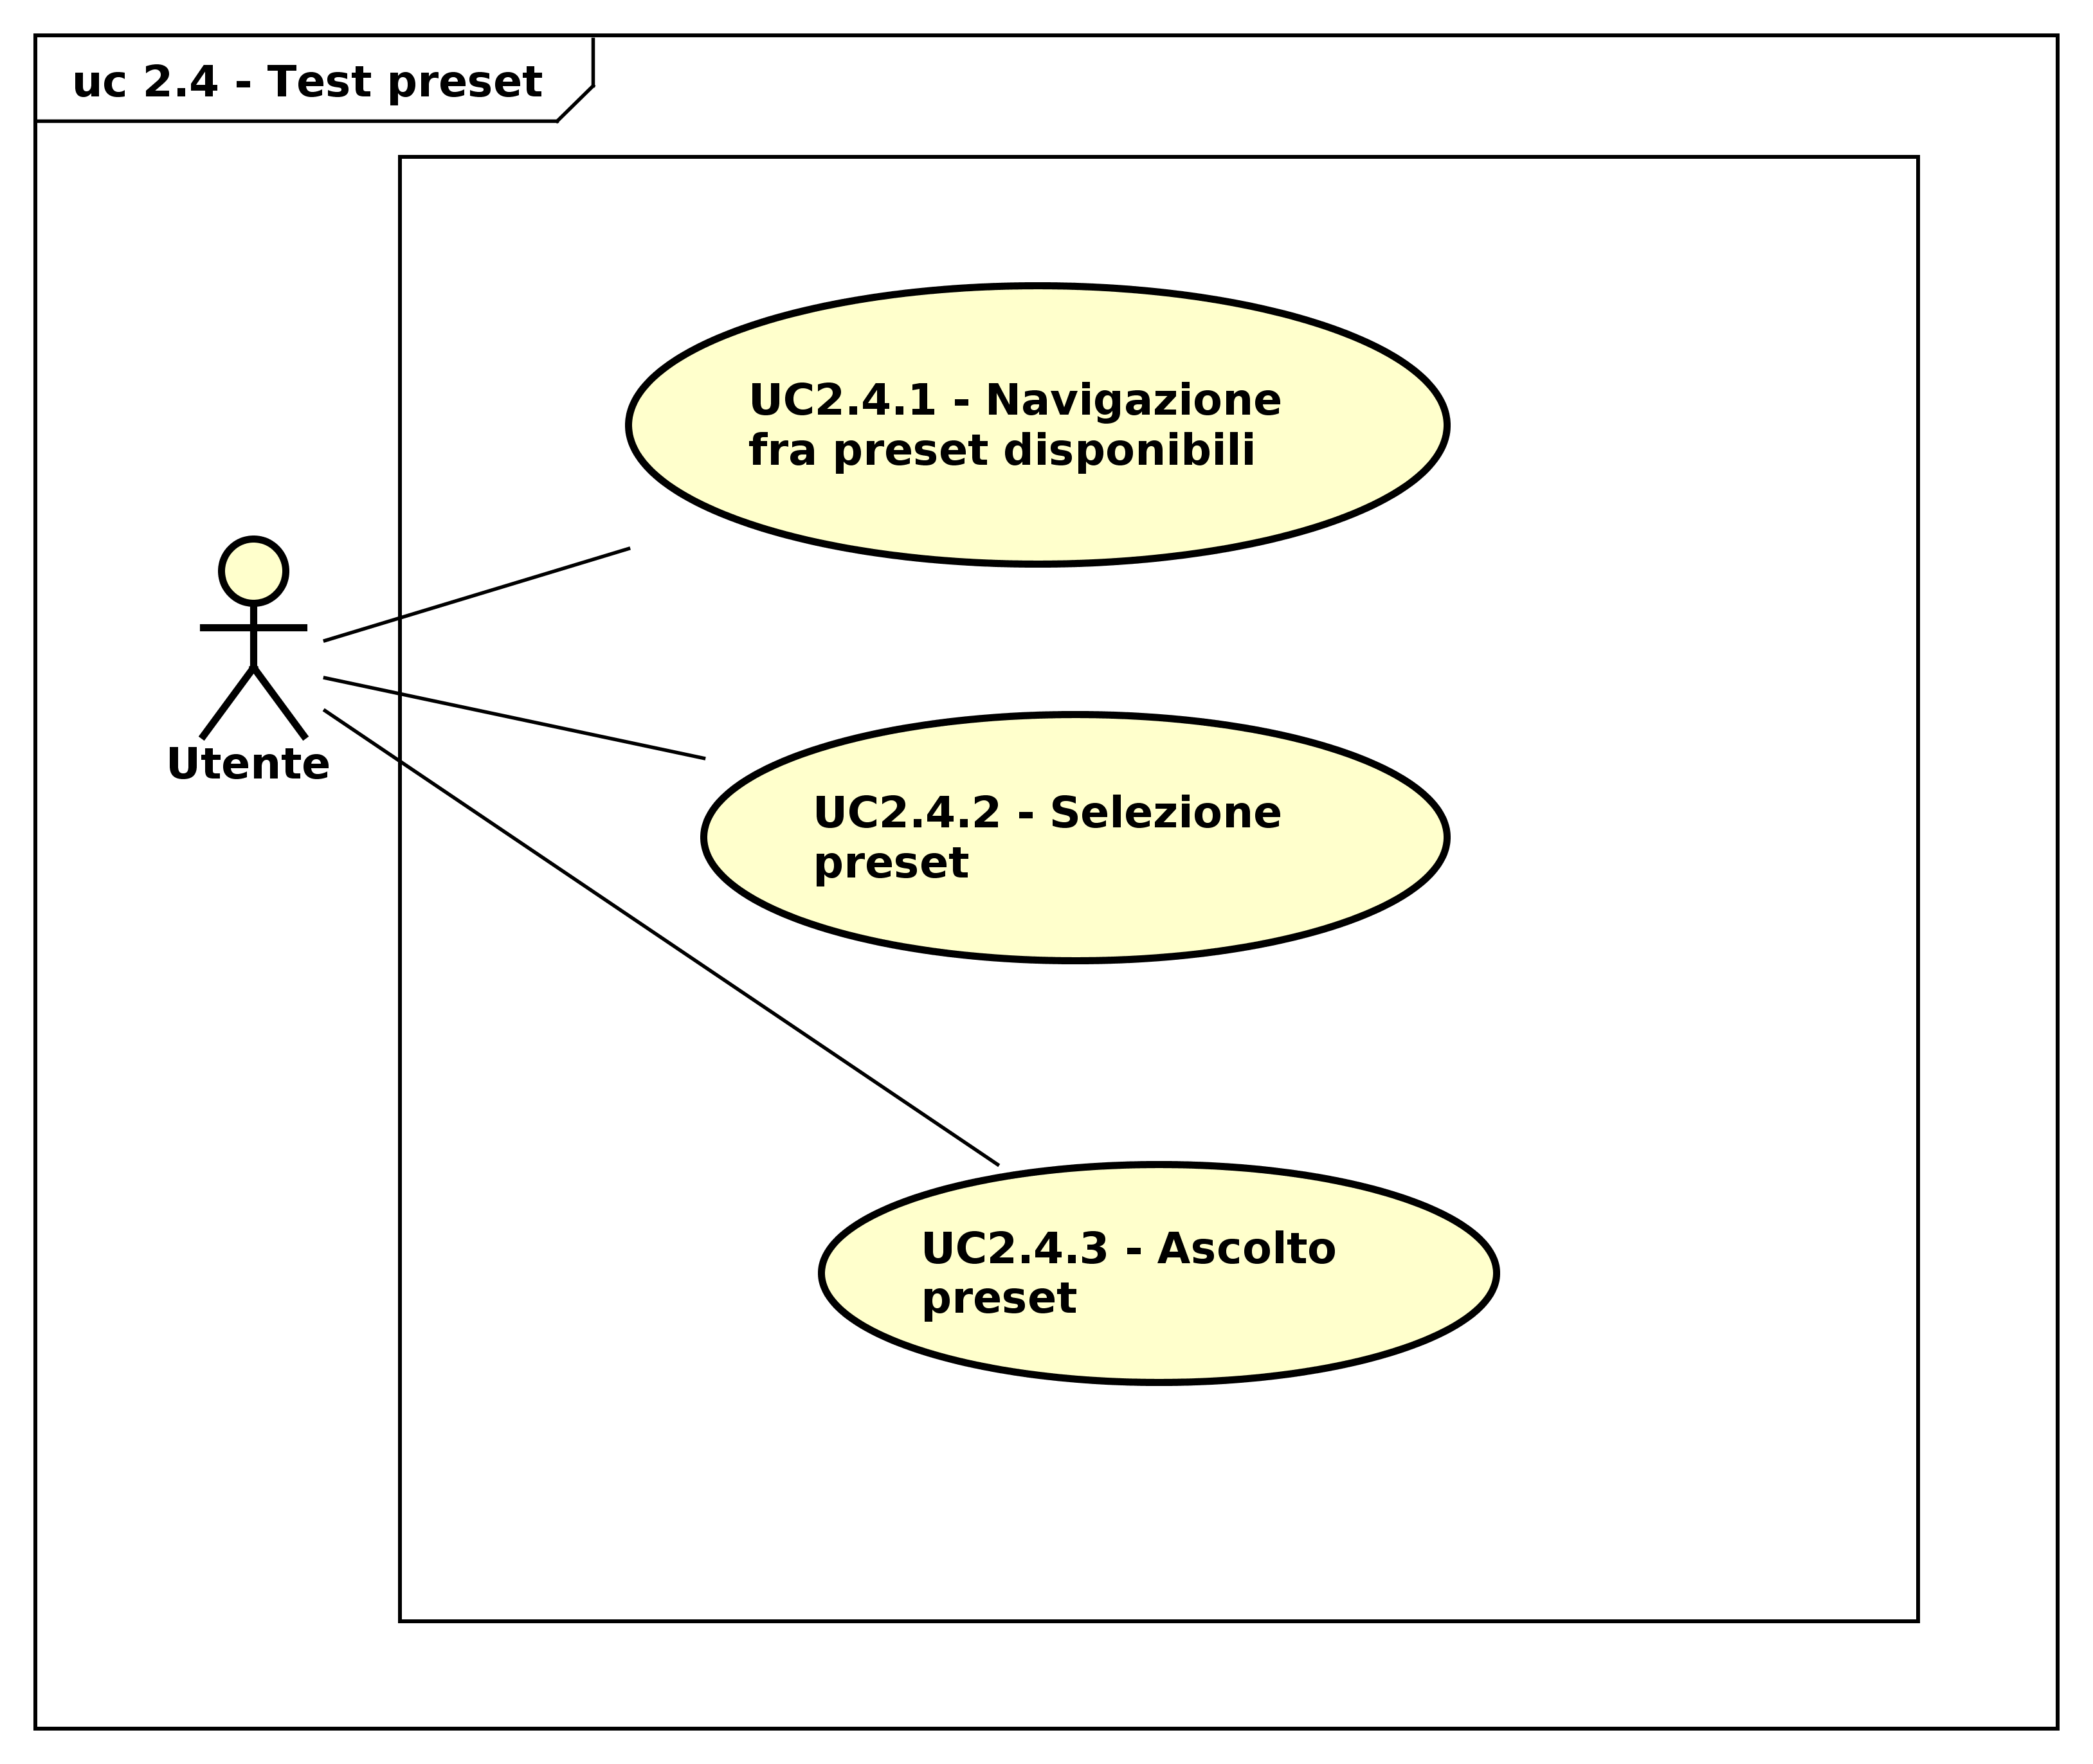
\includegraphics[scale=0.5]{UseCase_17_03_2016/immagini/uc_2_4_test_preset.png}
\captionsetup{labelfont=bf}
\caption{Caso d'uso UC2.4}
\end{figure}

\begin{itemize}
\item \textbf{Attori}: Utente;
\item \textbf{Scopo e descrizione}: l'utente può ascoltare il preset creato;
\item \textbf{Precondizione}: il preset è stato creato correttamente;
\item \textbf{Postcondizione}: il preset viene ascoltato.
\end{itemize}

\subsection{Caso d'uso UC2.5: Modifica preset}

\begin{figure}[htbp]
\centering
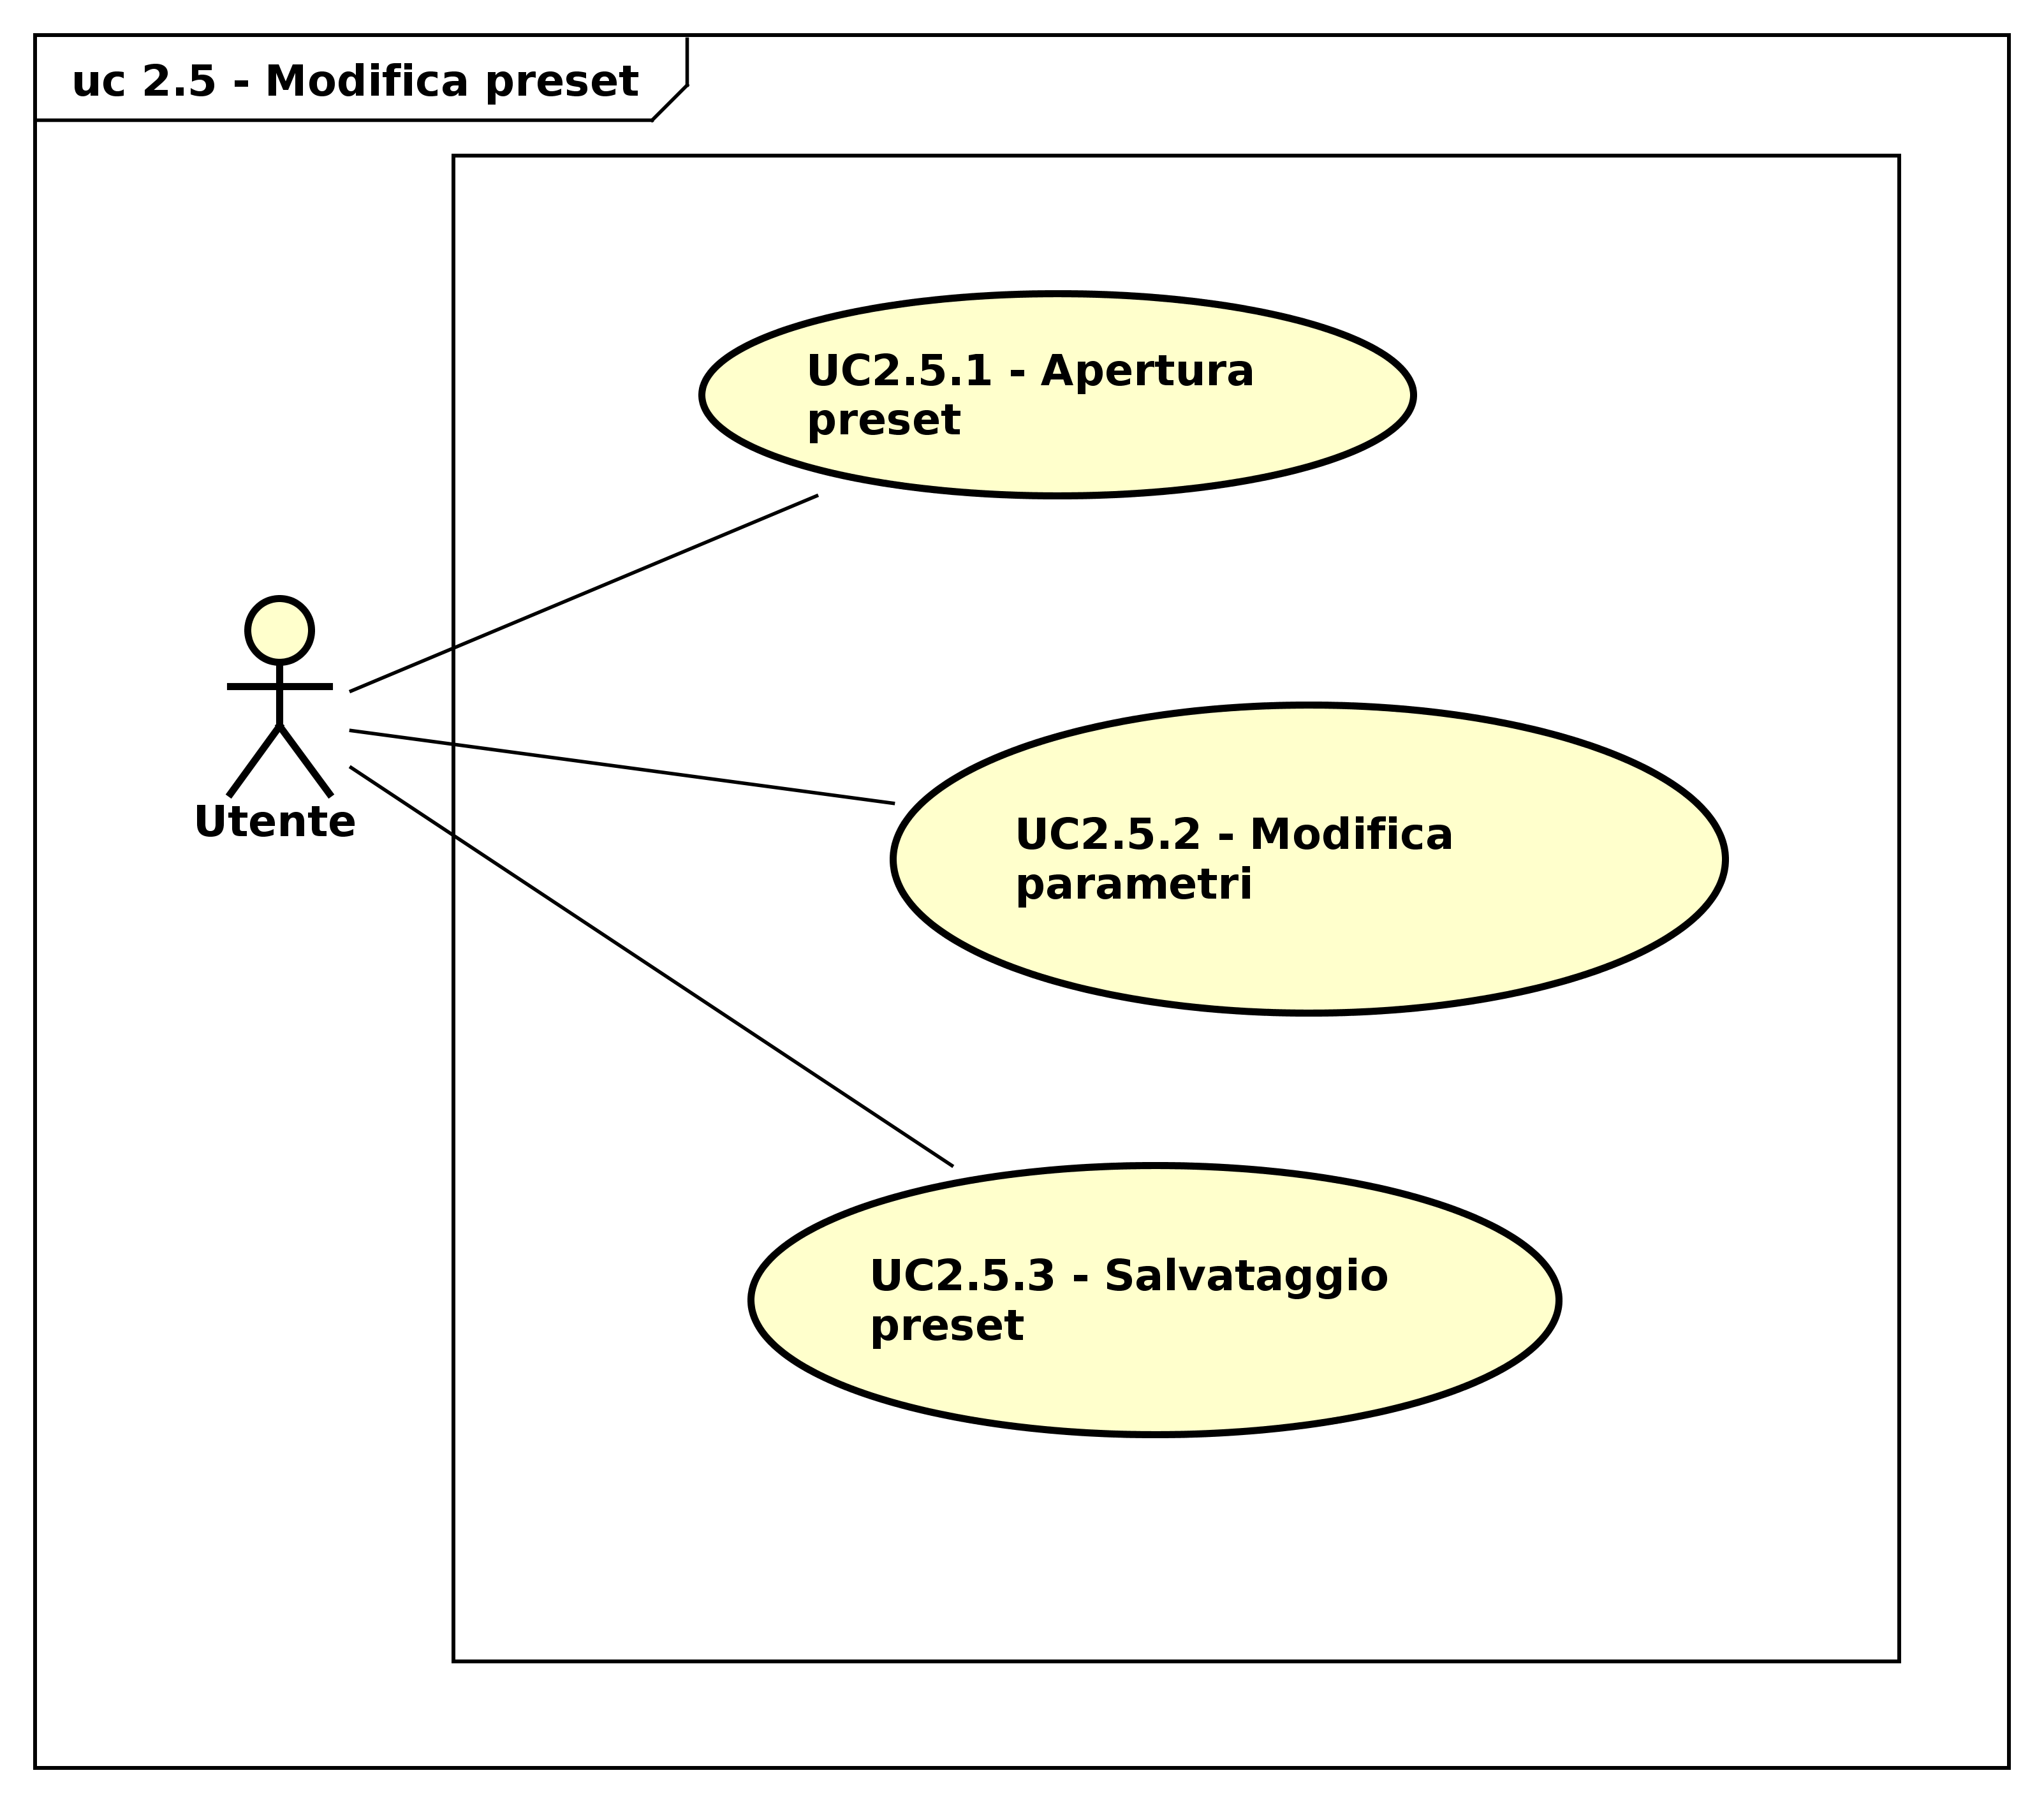
\includegraphics[scale=0.5]{UseCase_17_03_2016/immagini/uc_2_5_modifica_preset.png}
\captionsetup{labelfont=bf}
\caption{Caso d'uso UC2.5}
\end{figure}

\begin{itemize}
\item \textbf{Attori}: Utente;
\item \textbf{Scopo e descrizione}: l'utente può aprire un preset già creato e modificarlo;
\item \textbf{Precondizione}: viene selezionato un preset correttamente creato; 
\item \textbf{Flusso principale degli eventi}:
\begin{enumerate}
\item L'utente seleziona il preset da modificare (UC2.5.1);
\item L'utente modifica i parametri del preset (UC2.5.2);
\item L'utente salva le modifiche apportate (UC2.5.3).
\end{enumerate}
\item \textbf{Postcondizione}: il preset viene modificato e salvato correttamente.
\end{itemize}

\subsection{Caso d'uso UC3: Modulo di sistema alto livello}

\begin{figure}[htbp]
\centering
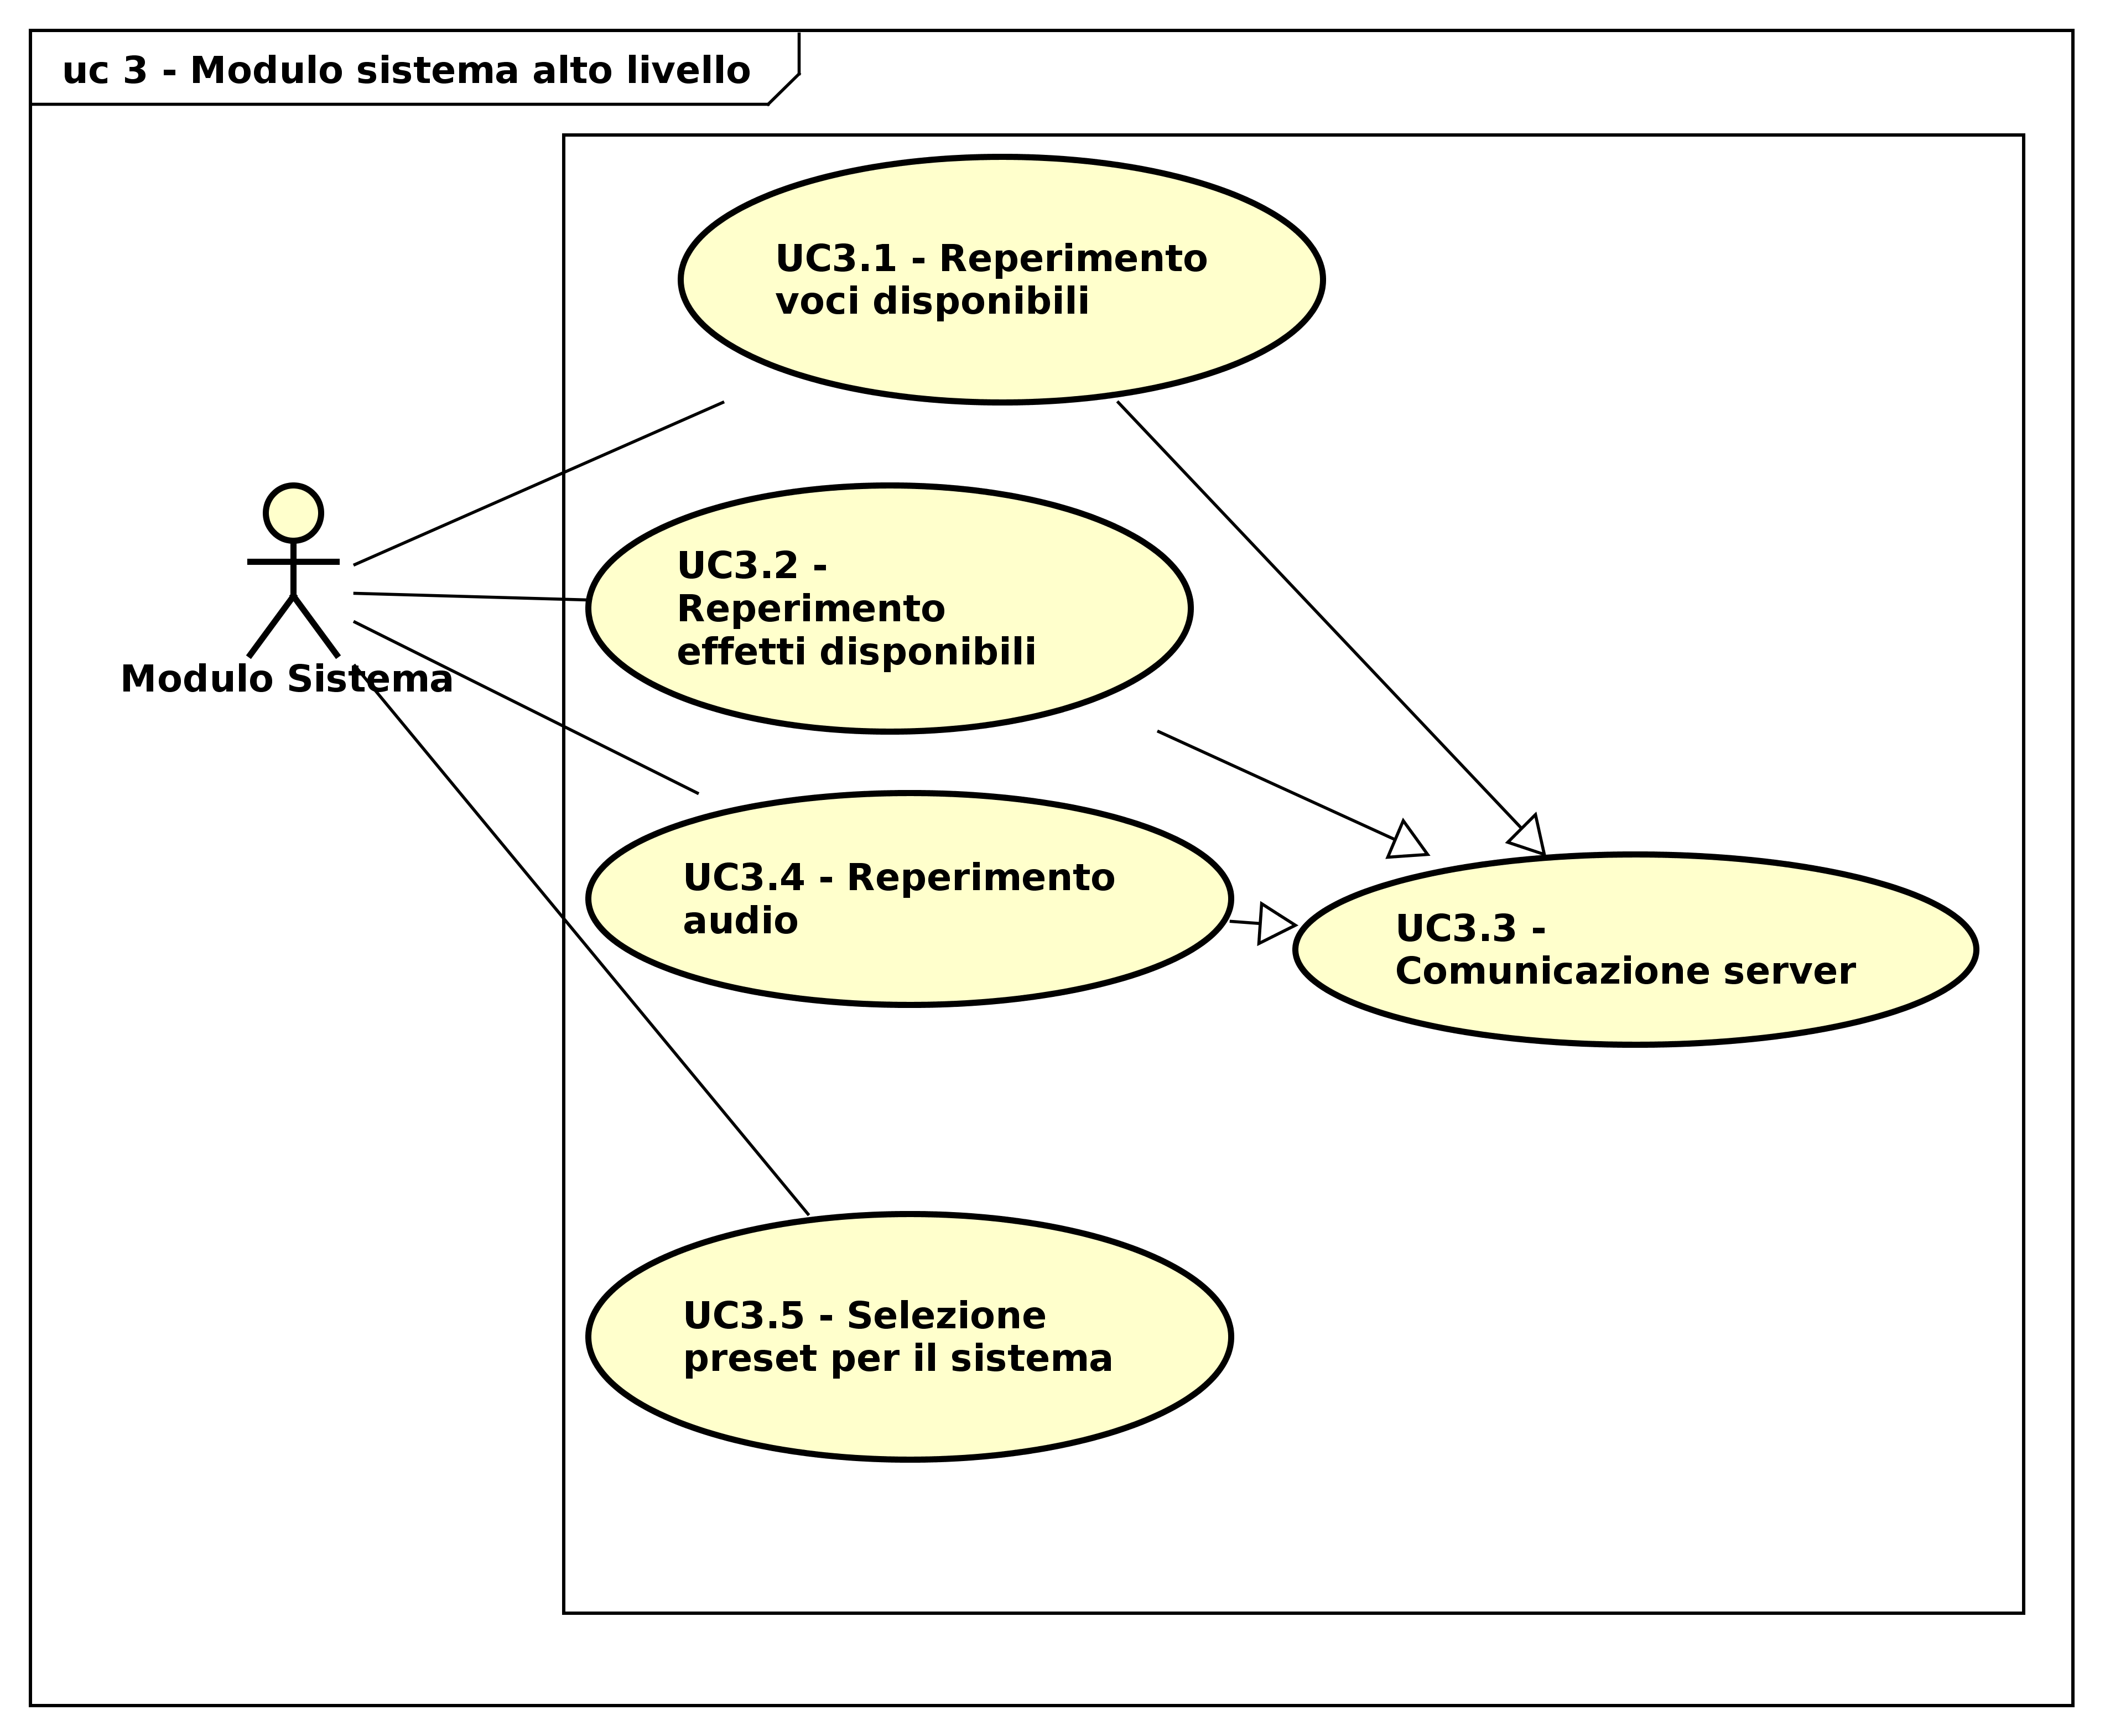
\includegraphics[scale=0.5]{UseCase_17_03_2016/immagini/uc_3_modulo_sistema_alto_livello.png}
\captionsetup{labelfont=bf}
\caption{Caso d'uso UC3}
\end{figure}

\begin{itemize}
\item \textbf{Attori}: Modulo di sistema;
\item \textbf{Scopo e descrizione}: il modulo di sistema può reperire gli effetti e le voci disponibili comunicando con il server;
\item \textbf{Precondizione}: il modulo è pronto ad operare;
\item \textbf{Postcondizione}: il modulo svolge quanto richiesto;
\end{itemize}

\subsection{Caso d'uso UC3.3: Comunicazione server}

\begin{figure}[htbp]
\centering
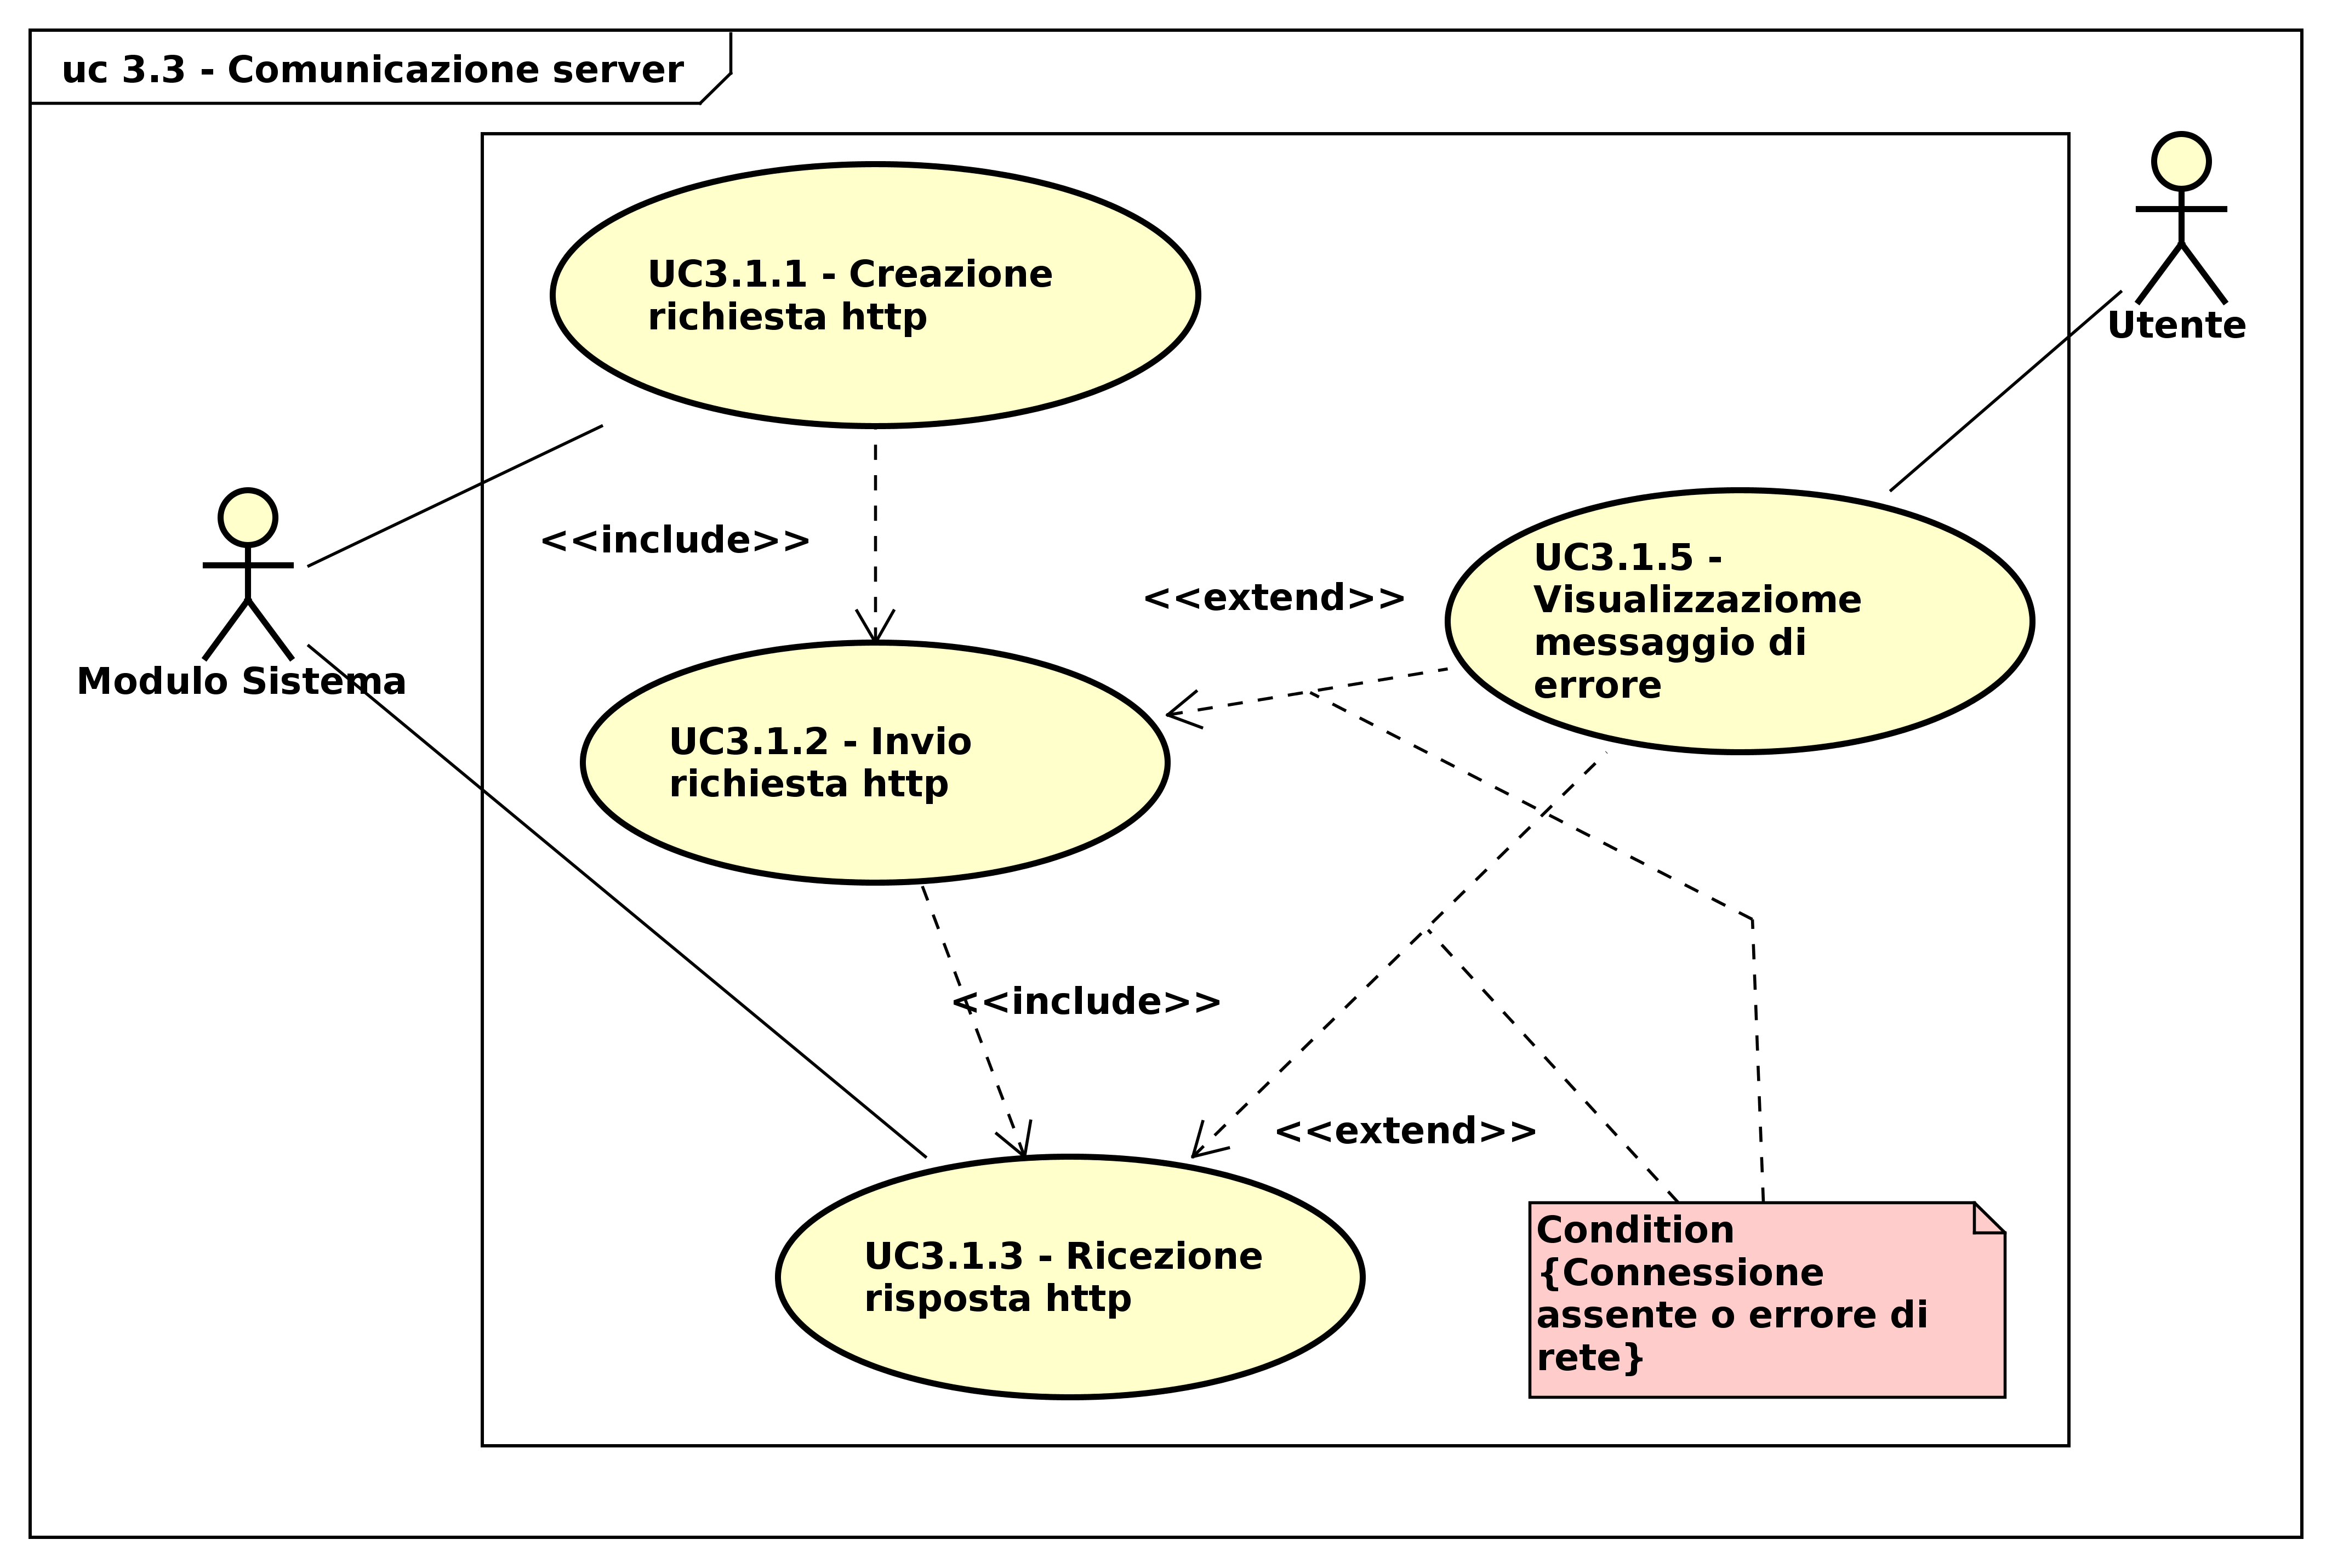
\includegraphics[scale=0.5]{UseCase_17_03_2016/immagini/uc_3_3_comunicazione_server.png}
\captionsetup{labelfont=bf}
\caption{Caso d'uso UC3.3}
\end{figure}

\begin{itemize}
\item \textbf{Attori}: Modulo di sistema, Utente;
\item \textbf{Scopo e descrizione}: il modulo di sistema crea una richiesta http, la invia al server e riceve da quest'ultimo una risposta;
\item \textbf{Precondizione}: il modulo è pronto a comunicare con il server;
\item \textbf{Flusso principale degli eventi}:
\begin{enumerate}
\item Il modulo crea una richiesta http (UC3.1.1);
\item Il modulo invia una richiesta http creata (UC3.1.2);
\item Il modulo riceve una risposta dal server (UC3.1.3).
\end{enumerate}
\item \textbf{Estensioni}: nel caso in cui non fosse possibile comunicare con il server a causa di assenza di connessione, il sistema avverte l'utente dell'errore;  
\item \textbf{Postcondizione}: la comunicazione va a buon fine;
\end{itemize}

\subsection{Caso d'uso UC3.5: Selezione preset}

\begin{figure}[htbp]
\centering
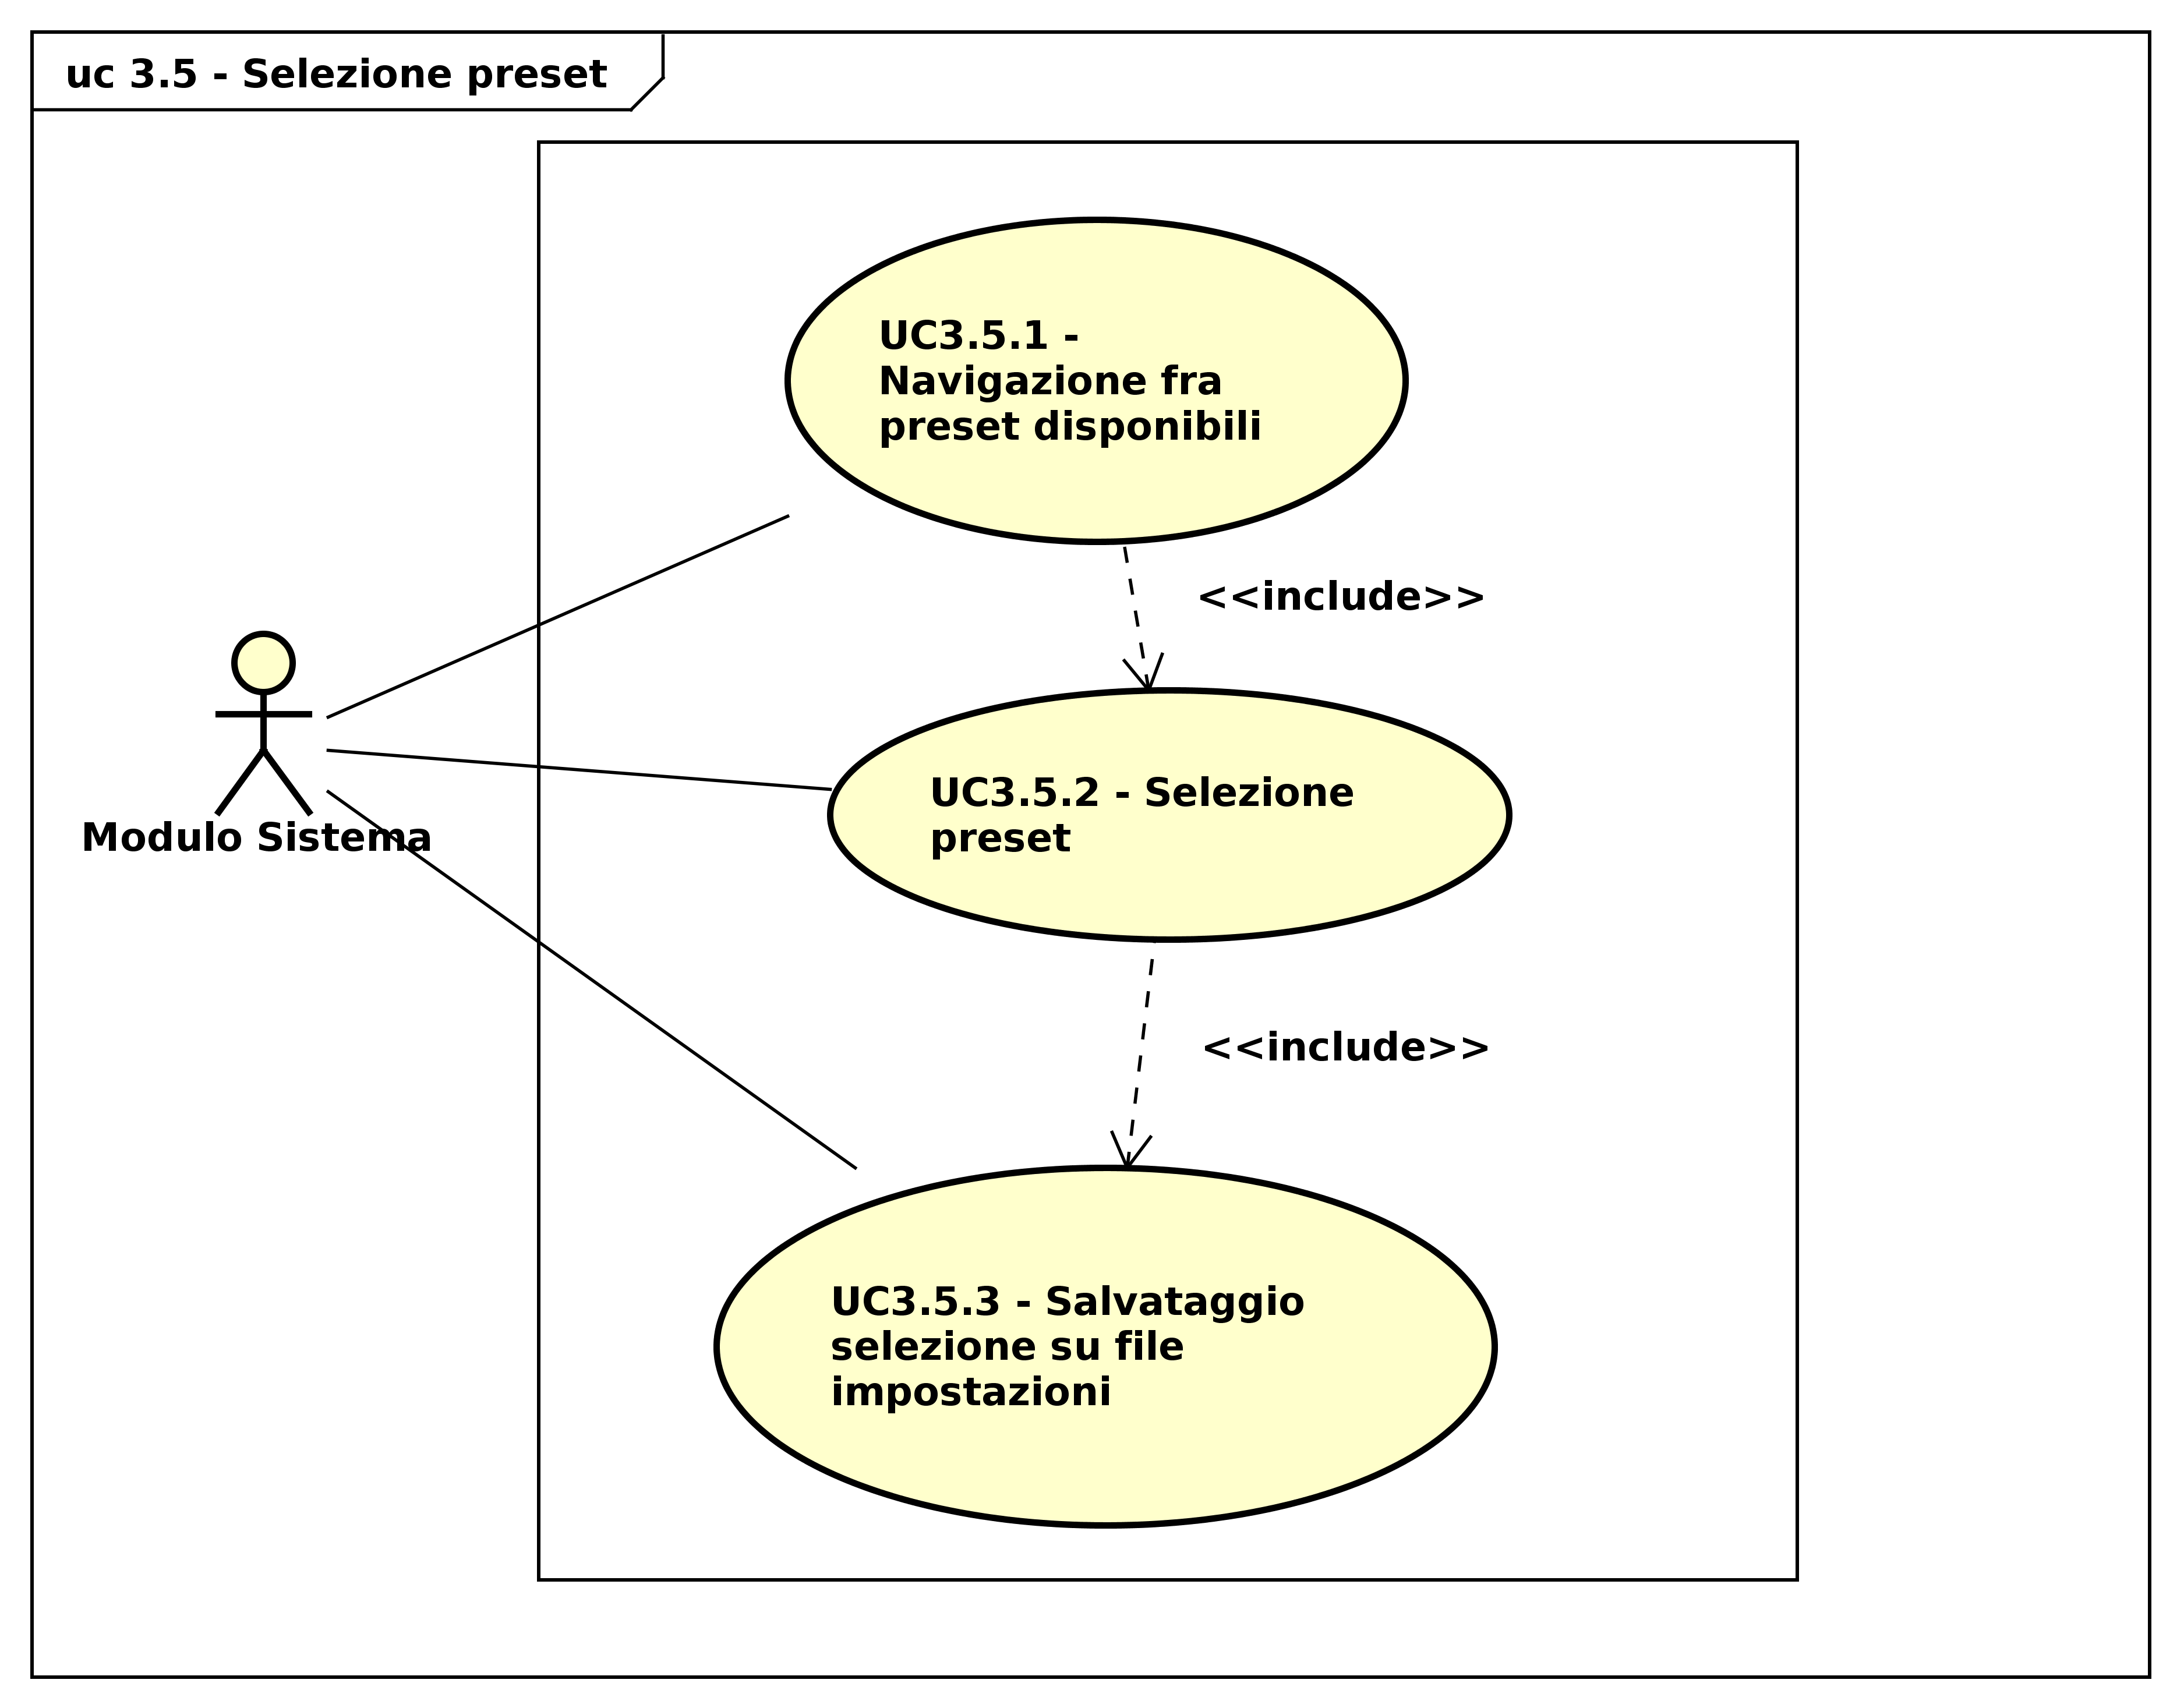
\includegraphics[scale=0.5]{UseCase_17_03_2016/immagini/uc_3_5_selezione_preset.png}
\captionsetup{labelfont=bf}
\caption{Caso d'uso UC3.5}
\end{figure}

\begin{itemize}
\item \textbf{Attori}: Modulo di sistema;
\item \textbf{Scopo e descrizione}: il modulo di sistema salva il preset selezionato su file di impostazioni;
\item \textbf{Precondizione}: esiste almeno un preset disponibile;
\item \textbf{Postcondizione}: il preset è stato selezionato e impostato.
\end{itemize}
\section{Requisiti}
\textbf{introduzione}..

\subsection{Requisiti funzionali}
\begin{center}
\def\arraystretch{1.6}
\bgroup
\begin{longtable}{| p{2.5cm} | p{3cm} | p{5.25cm} | p{2cm} |}
\hline
\textbf{Requisito} & \textbf{Tipologia} & \textbf{Descrizione} & \textbf{Fonti}\\ \hline \hline 

R0F1 & Funzionale \newline Obbligatorio &
Il programma deve permettere la creazione di sceneggiati & 
Capitolato \newline UC1 \newline UC1.1\\ \hline

R0F1.6 & Funzionale \newline Obbligatorio & L'utente deve poter assegnare un titolo allo sceneggiato & UC1.1.6 \\ \hline

R1F1.6.1 & Funzionale \newline Desiderabile & L'utente deve poter modificare il titolo ad uno sceneggiato & UC1.1.6 \newline UC1.8 \\ \hline 

R0F1.1 & Funzionale \newline Obbligatorio & L'utente deve poter creare un nuovo personaggio per lo sceneggiato & UC1.1.1 \\ \hline

R0F1.1.1 & Funzionale \newline Obbligatorio & L'utente deve poter assegnare un nome al personaggio creato & UC1.1.1.1 \\ \hline

R1F1.1.2 & Funzionale \newline Desiderabile & L'utente deve poter modificare il nome associato ad un personaggio & UC1.1.1.1 \newline UC1.8 \\ \hline 

R0F1.1.3 & Funzionale \newline Obbligatorio & L'utente deve poter assegnare un avatar al personaggio creato & UC1.1.1.3 \\ \hline

R1F1.1.4 & Funzionale \newline Desiderabile & L'utente deve poter cambiare l'avatar al personaggio creato & UC1.1.1.3 \\ \hline

R0F1.1.1.3 & Funzionale \newline Obbligatorio & L'utente deve poter aprire un'immagine & UC1.7.1 \newline UC1.1.1.3 \\ \hline


\caption{Requisiti funzionali}
\end{longtable}

\egroup
\end{center}

%\input {sections/nomesezione}
%\newpage

% ...

%\printglossaries

\end{document}
